
\chapter{LA CAPA DE RED}

	\par La capa de red se encarga de llevar los paquetes todo el camino, desde el origen hasta el destino. Para llegar al destino tal vez sea necesario realizar muchos saltos en el camino por enrutadores intermedios. Esta función ciertamente contrasta con la de la capa de enlace de datos, cuya única meta es mover tramas de un extremo del cable al otro. Por lo tanto, la capa de red es la capa más baja que maneja la transmisión de extremo a extremo.

	\par Para lograr sus objetivos, la capa de red debe conocer la topología de la red (es
decir, el conjunto de todos los enrutadores y enlaces) y elegir las rutas apropiadas
incluso para redes más grandes. También debe tener cuidado al escoger las rutas para
no sobrecargar algunas de las líneas de comunicación y los enrutadores, y dejar
inactivos a otros. Por último, cuando el origen y el destino están en redes diferentes, ocurren nuevos problemas. La capa de red es la encargada de solucionarlos. En este capítulo estudiaremos todos estos temas y los ilustraremos, principalmente mediante el uso de Internet y su protocolo de capa de red, IP.

\section{Aspectos de diseño de la capa de red}

	\subsection{Servicios proporcionados a la capa de transporte}

		\par La capa de red proporciona servicios a la capa de transporte en la interfaz entre la 
capa de red y de transporte. Una pregunta importante es qué tipo de servicios 
proporciona precisamente la capa de red a la capa de transporte. Hay que diseñar los 
servicios de manera cuidadosa, con los siguientes objetivos en mente:
	\begin{itemize}
		\item Los servicios deben ser independientes de la tecnologia del 			
		enrutador.
		\item La capa de transporte debe estar aislada de la cantidad, tipo y topología 
		de los enrutadores presentes.
		\item Las direcciones de red disponibles para la capa de transporte deben usar 
		un plan de numeracin uniforme, incluso a traves de redes LAN y WAN.
	\end{itemize}
	
\par Dadas estas metas, los diseñadores de la capa de red tienen mucha libertad para 
escribir especificaciones detalladas de los servicios que se ofrecerán a la capa de 
transporte. Con frecuencia esta libertad degenera en una batalla campal entre dos 
bandos en conflicto. La discusión se centra en determinar si la capa de red debe 
proporcionar un servicio orientado a conexión o un servicio sin conexión.
\par Estos dos bandos son:
	\begin{enumerate}
		\item La comunidad de internet
		\begin{itemize}\itemsep=0pt
			\item La tarea del enrutador es solo mover bits de un lado a otro.
			\item La subred es inherentemente inestable. Los hosts deben efectuar el 
			control de errores y el control de flujo.
			\item No debe efectuarse ningún ordenamiento de paquetes.
			\item Cada paquete se transportará de manera independiente a sus 
			antecesores.
			\end{itemize}
		\item Las compañías telefónicas:
		\begin{itemize}\itemsep=0pt
			\item La subred debe proporcionar un servicio confiable, orientado a la
conexión..
			\item La subred es inherentemente inestable. Los hosts deben efectuar el 
			control de errores y el control de flujo.
			\item La calidad del servicio es el factor dominante, sin conexiones en la 
			subred tal calidad es muy difícil de alcanzar, especialmente para el tráfico de 
			tiempo real como la voz y el video.
		\end{itemize}
	\end{enumerate}
\par Los dos bandos se ejemplifican con Internet y las redes ATM.

\subsection{Implementación del servicio sin conexión}
	\begin{itemize}\itemsep=0pt
			\item Los paquetes se colocan individualmente en la subred y se enrutan de
manera independiente.  Por eso debe levar una dirección de destino completa. 
			\item \textbf{Datagramas} = paquetes
			\item \textbf{Subred de Datagramas} = subred
			\item Tabla interna de un enrutador
			\par Entrada de la tabla interna = (destino, línea de salida)
			\par Cuando llega un paquete: Se lo almacena y se comprueba que llegó bien; se reenvía al destino de acuerdo con la tabla del enrutador.
			\item Los enrutadores requieren la capacidad de reemplazar identificadores de conexión en los paquetes salientes, ya que podria darse el caso de que un host H1 inicie una conexión con identificador 1; luego otro host H3 inicia conexión con identificador 1, y ambos hosts están conectados al mismo enrutador A.
			\end{itemize}
			
	\par Ahora veamos como funciona una red de datagramas. Suponga que el proceso P1 de la figura tiene un mensaje largo para P2. Dicho proceso entrega el mensaje a la capa de transporte y le indica a ésta que lo envíe al proceso P2 en el host H2. El código de la capa de transporte se ejecuta en H1, por lo general dentro del sistema operativo. Dicho código agrega un encabezado de transporte al frente del mensaje y entrega el resultado a la capa de red, que quizá sólo sea otro procedimiento dentro del sistema operativo.

	\begin{center} 
		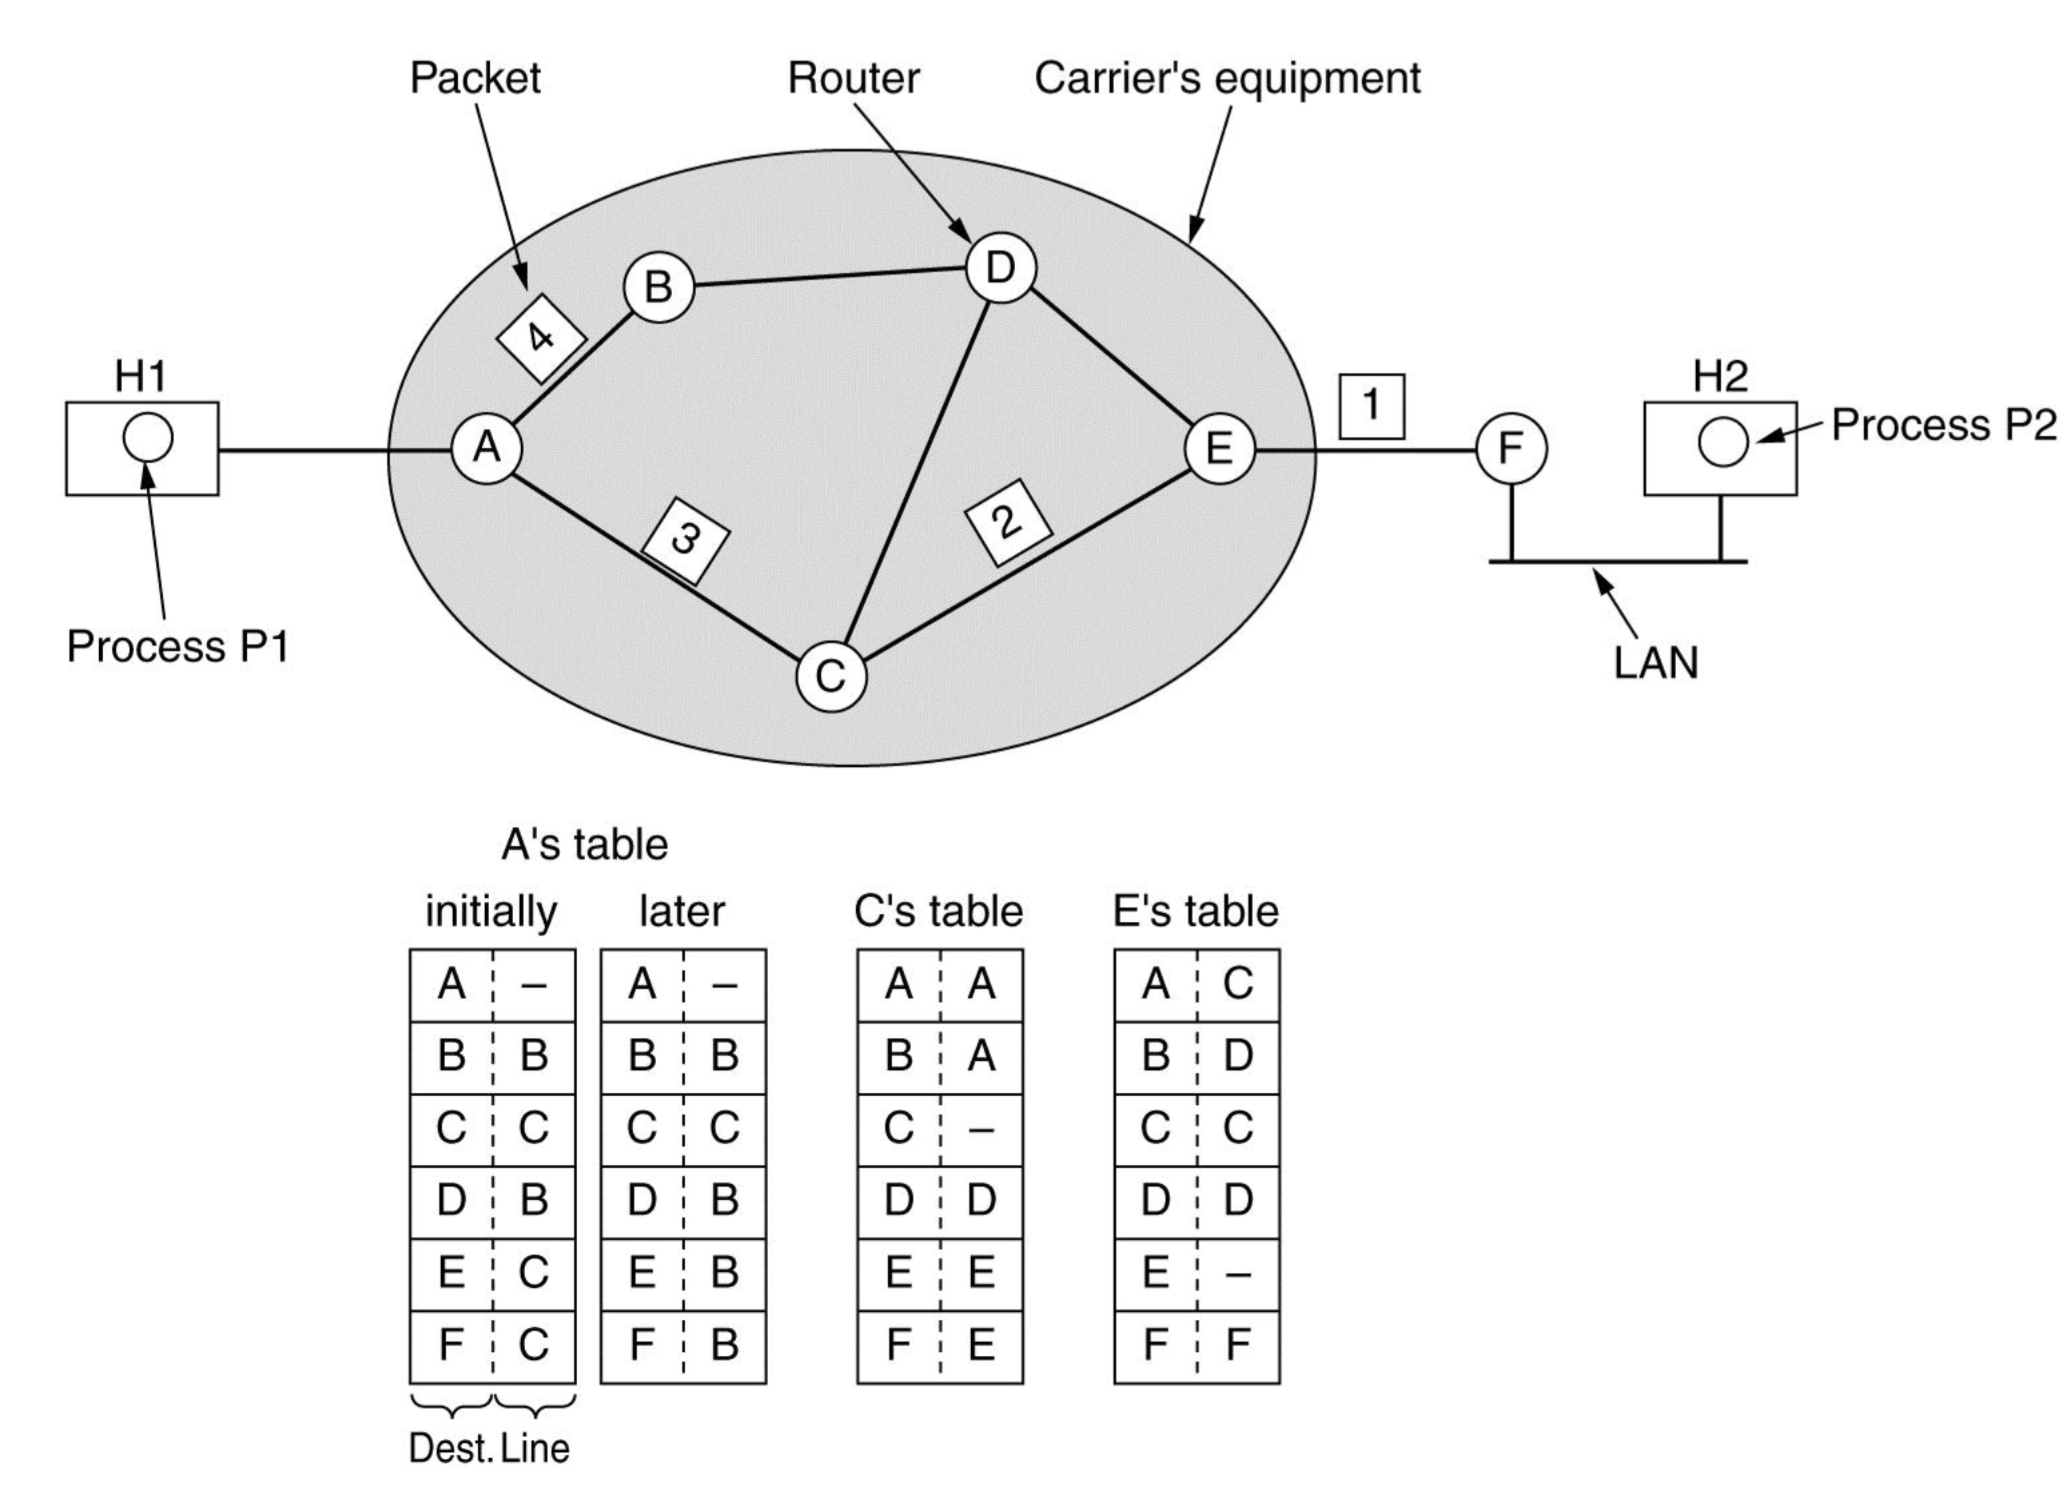
\includegraphics[width=8cm, height=6cm]{./imagenes/norientado.png} 
	\end{center}

	\par Problema:  
	\par IP es el ejemplo dominante de un servicio de red sin conexión. Cada paquete 
transporta una dirección IP de destino que los enrutadores usan para reenviar cada 
paquete por separado. Las direcciones son de 32 bits en los paquetes IPv4 y de 128 
bits en los paquetes IPv6.

\subsection{Implementación del servicio orientado a conexión}
	\begin{itemize}\itemsep=0pt
			\item \textbf{Conexiónes o circuitos virtuales (CV)}
			\item \textbf{Subred de Circuitos Virtuales} = subred
			\item Evitar la necesidad de elegir una nueva ruta para cada paquete enviado. 
			La ruta de una conexión se almacena en tablas en los enrutadores, esta ruta se 
			usa para todo el tráfico que fluye a través de la conexión.
			\item Cada paquete lleva un identificador de CV.
			\item Liberación de conexión: se termina el CV
			\item Se paga el precios del espacio de tabla en los enrutadores. El uso de CVs 
			requiere una fase de configuración que consume tiempo y recursos.
	\end{itemize}

\begin{center} 
	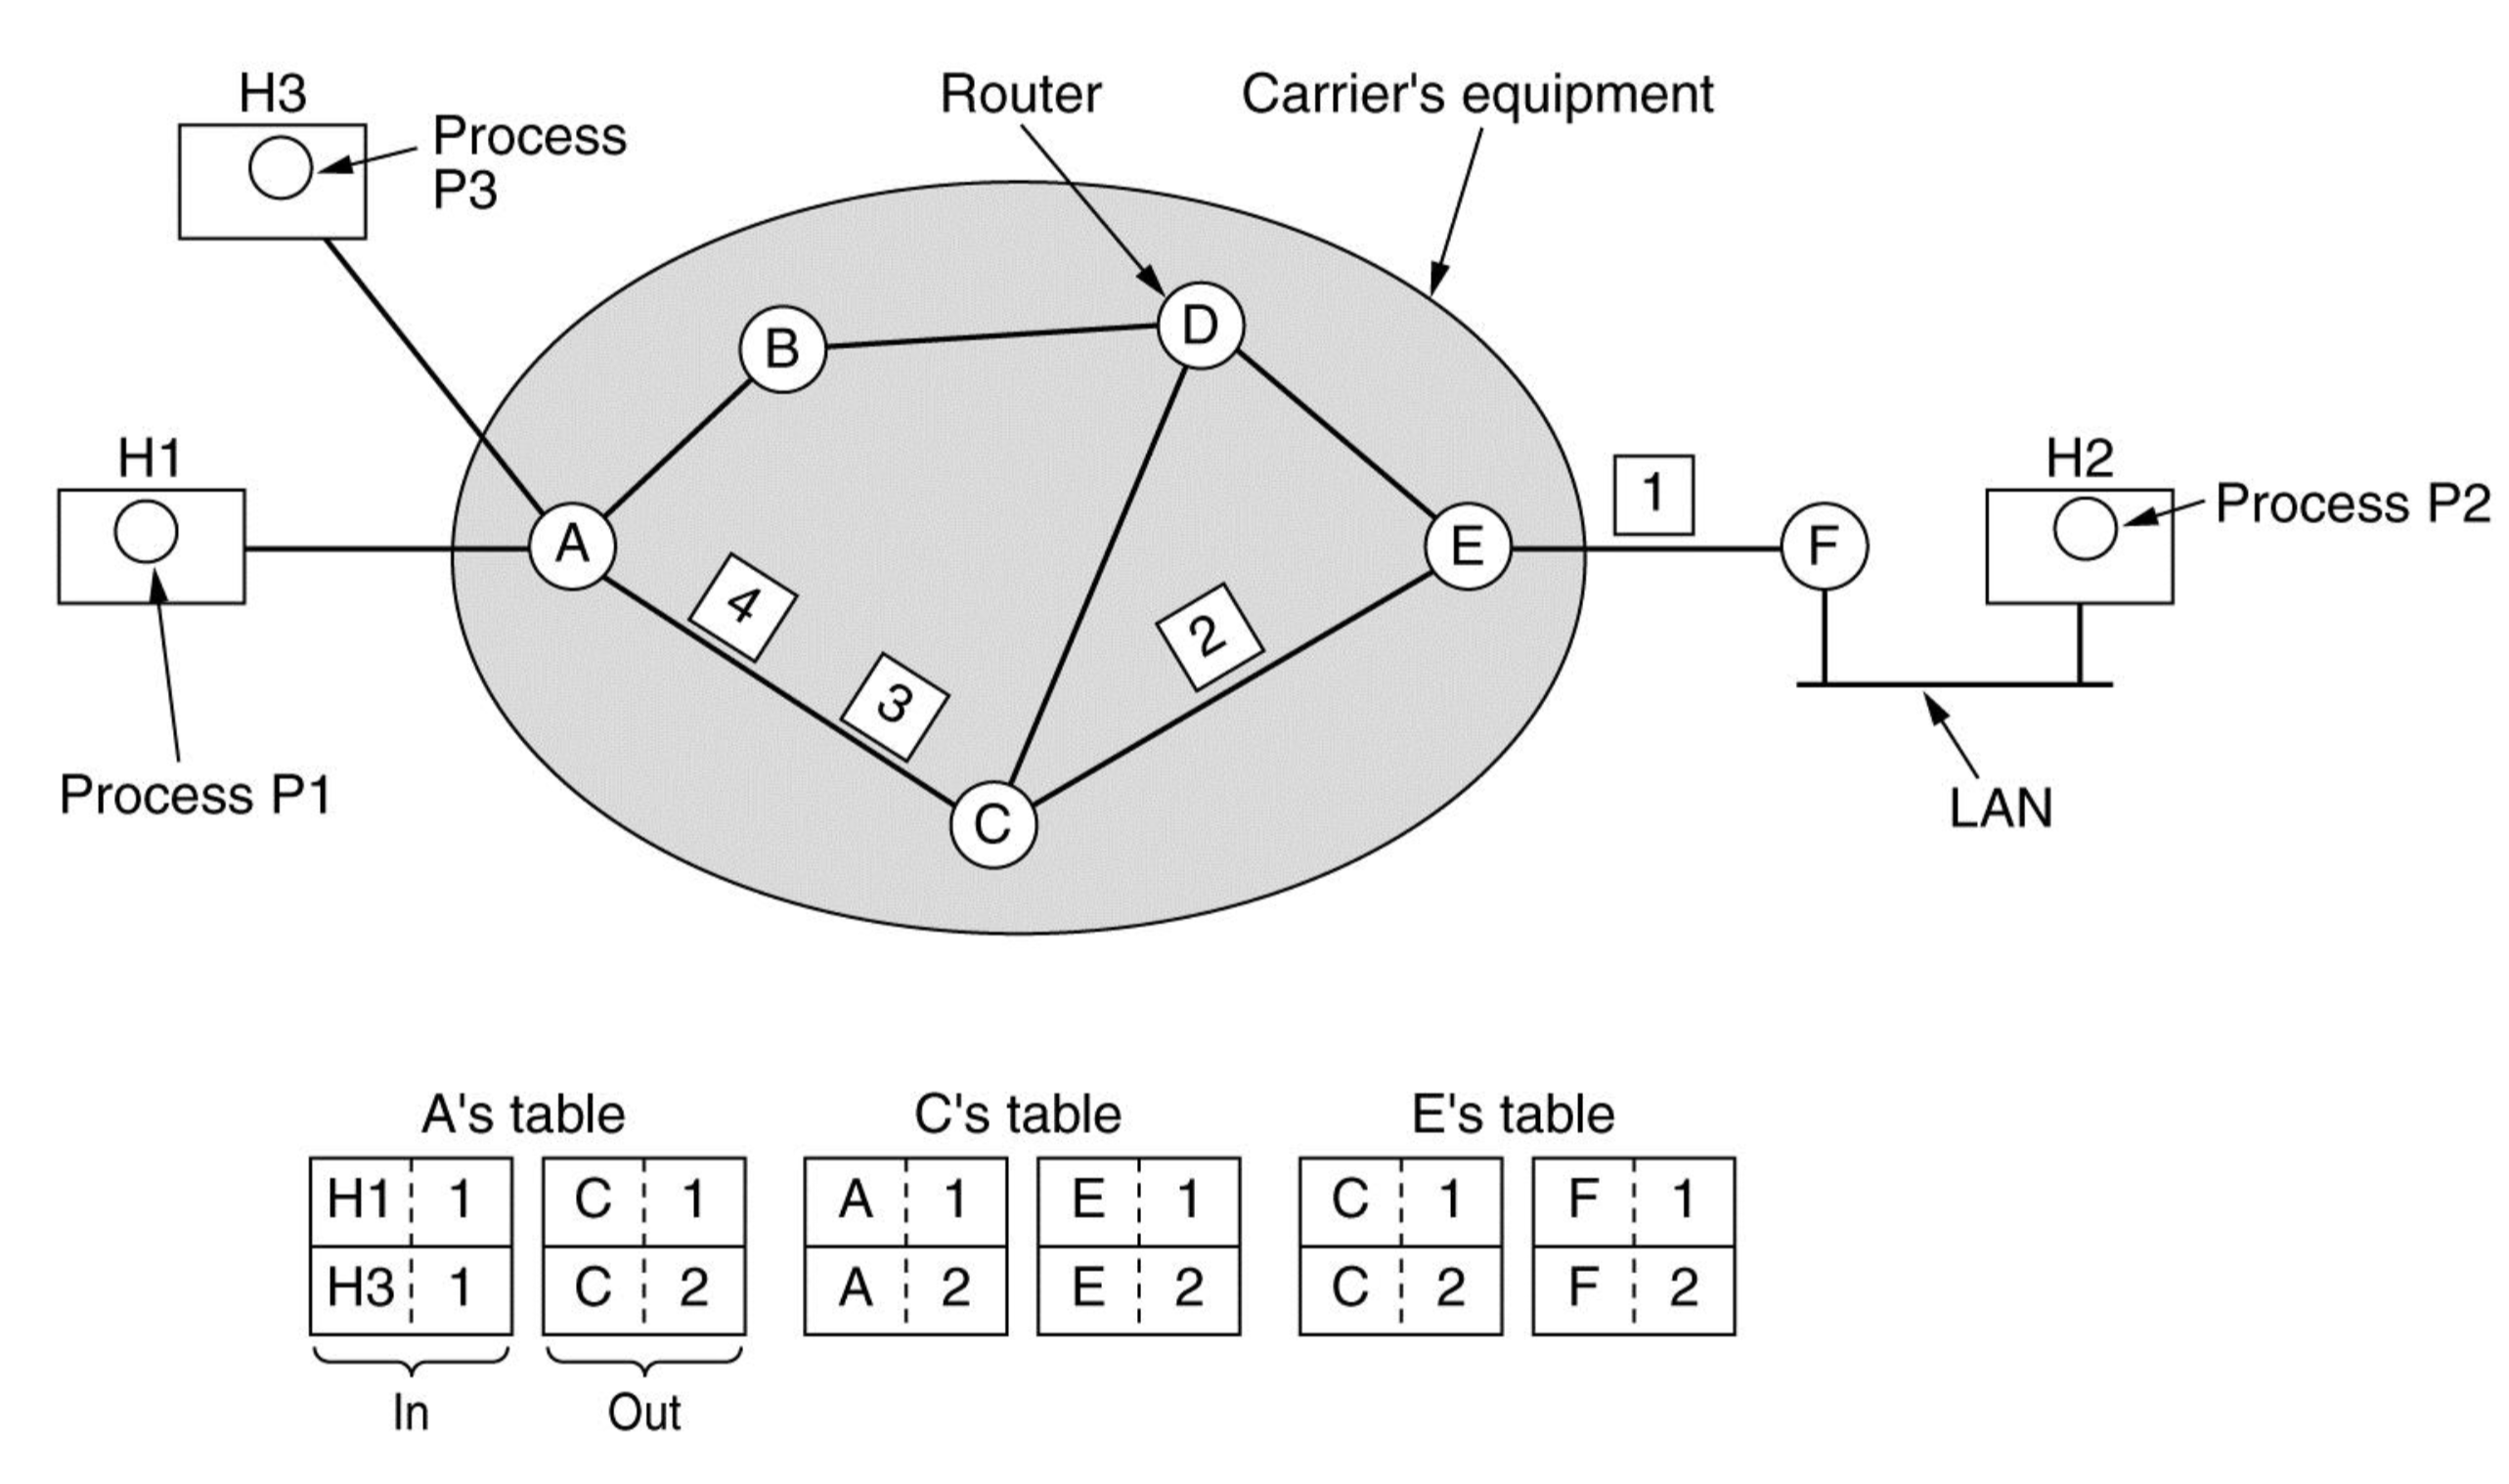
\includegraphics[width=8cm, height=6cm]{./imagenes/orientado.png} 
\end{center}

\par En algunos contextos, a este proceso se le conoce como conmutación mediante 
etiquetas. MPLS (MultiProtocol Label Swithching) es un ejemplo de servicio de red 
orientado a conexión. Se utiliza dentro de las redes de ISP en Internet, en donde los 
paquetes IP se envuelven en un encabezado MPLS que tiene un identificador de 
conexión o etiqueta de 20 bits.
	
\subsection{Comparación entre las redes de circuitos virtuales y las redes de datagramas}
	Dentro de la red existen ventajas y desventajas entre los circuitos virtuales y los 
	datagramas. Una de ellas tiene que ver con el tiempo de configuración y el tiempo de 
	análisis de la dirección. El uso de circuitos virtuales requiere una fase de 
	configuración que necesita tiempo y recursos. Sin embargo, una vez que se paga 
	este precio, es fácil averiguar qué hacer con un paquete de datos en una red de 
	circuitos virtuales: el enrutador sólo usa el número de circuito para buscar en una 
	tabla y encontrar hacia donde va el paquete. En una red de datagramas no se 
	requiere configuración, pero se requiere un procedimiento más complicado para 
	localizar la entrada correspondiente al destino.

	\begin{center} 
		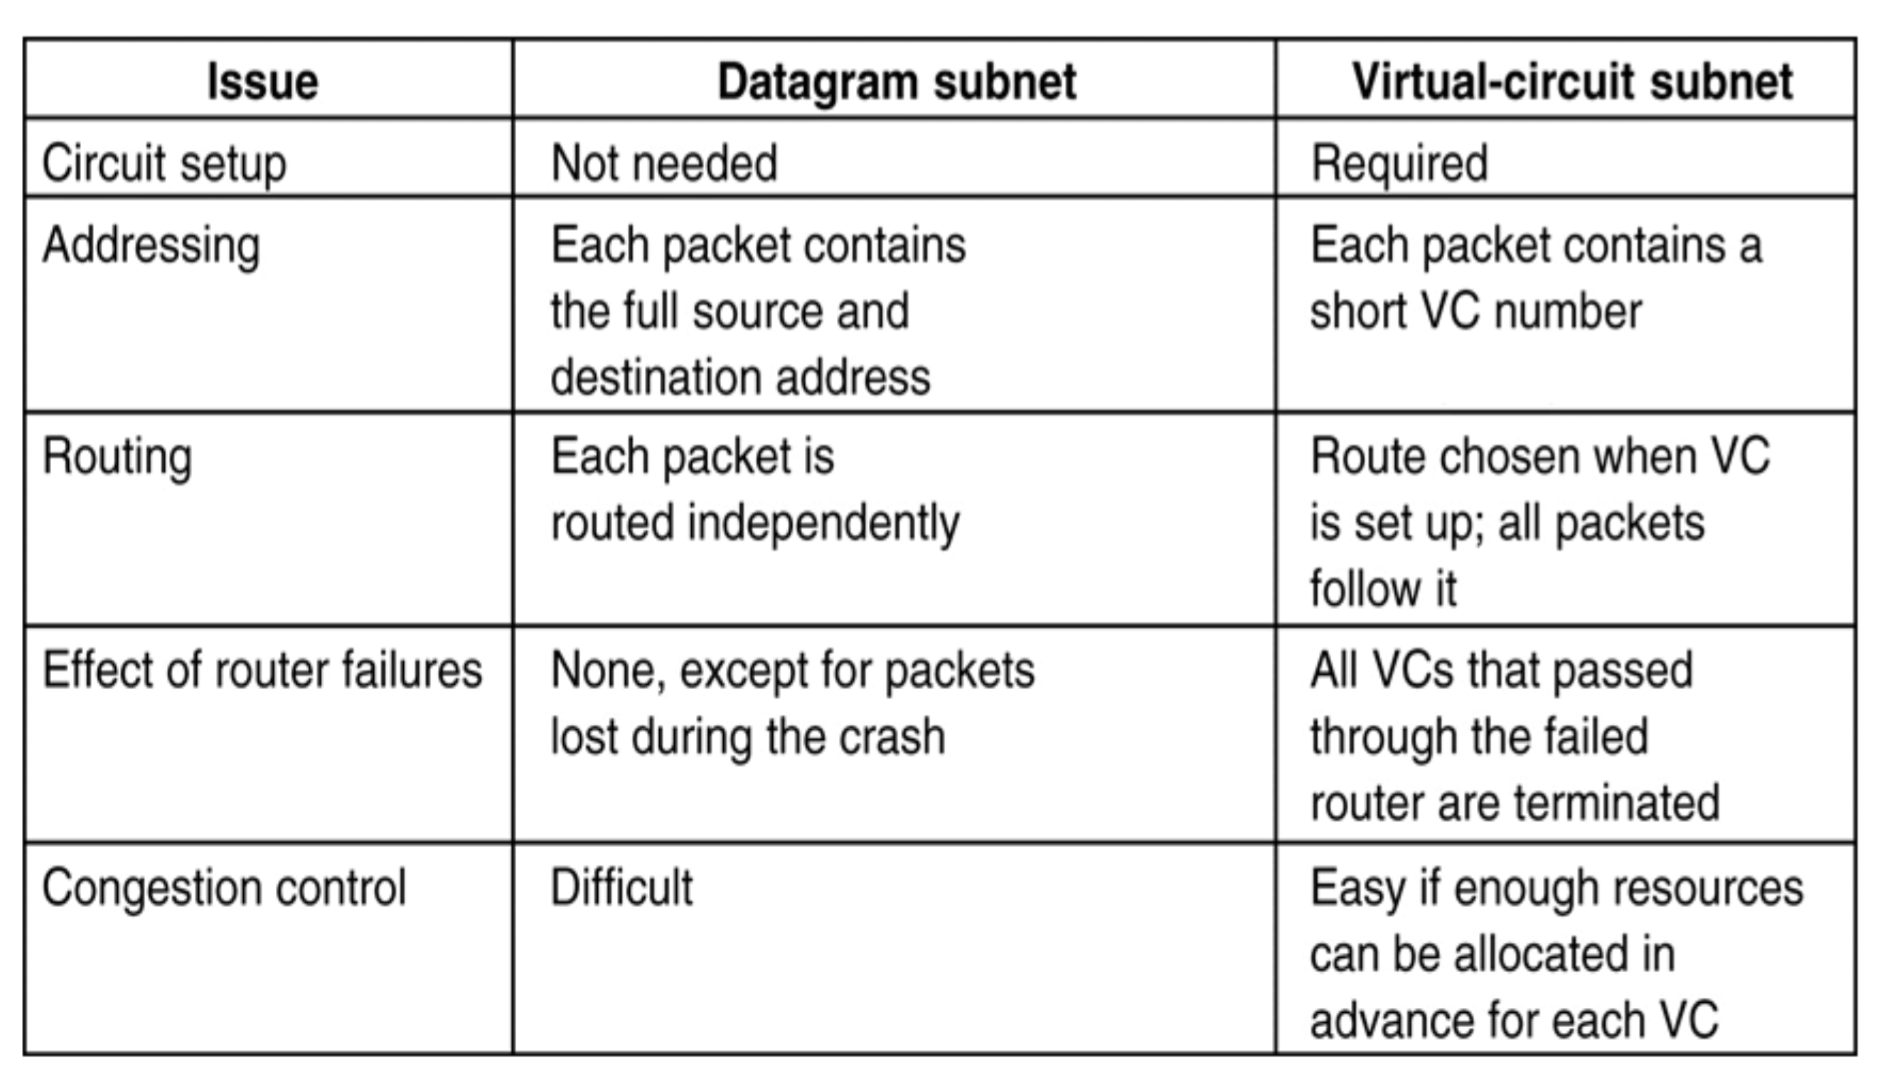
\includegraphics[width=10cm, height=6cm]{./imagenes/comparacion.png}
	\end{center}
	
	\begin{itemize}
		\item Si se cae un enrutador en CV: se pierde su memoria, y todos los CV que 
		pasan por el tendrán que abortarse.
		\item Si se cae un enrutador de datagramas: solo sufrirán los usuarios cuyos 
		paquetes estaban encolados en el enrutador en el momento de la falla, 
		dependiendo de si había confirmado o no su recepción, tal vez ni siquiera todos 
		ellos.
	\end{itemize}


\section{Algoritmos de enrutamiento}
	\par El algoritmo de enrutamiento es aquella parte del software de la capa de red 
	responsable de decidir por cuál línea de salida transmitirá un paquete entrante. Si la 
	red usa datagramas de manera interna, esta decisión debe tomarse cada vez que 
	llega un paquete de datos, dado que la mejor ruta podría haber cambiado desde la 
	última vez. Si la red usa circuitos virtuales internamente, las decisiones de 
	enrutamiento se toman sólo al establecer un circuito virtual nuevo. En lo sucesivo, 
	los paquetes de datos simplemente siguen la ruta ya establecida. Este último caso a 
	veces se llama enrutamiento de sesión, dado que una ruta permanece vigente 
	durante toda una sesión.
	
	\par En ocasiones es útil distinguir entre el enrutamiento, que es el proceso que 
	consiste en tomar la decisión de cuáles rutas utilizar, y el reenvío, que consiste en la 
	acción que se toma cuando llega un paquete. Podemos considerar que un enrutador 
	tiene dos procesos internos. Uno de ellos maneja cada paquete conforme llega, y 
	después busca en las tablas de enrutamiento la línea de salida por la cual se enviará. 
	Este proceso se conoce como reenvío. El otro proceso es responsable de llenar y 
	actualizar las tablas de enrutamiento. Es ahí donde entra en acción el algoritmo de 
	enrutamiento.
	
	\par Propiedades que todo algoritmo de enrutamiento debe poseer:
		\begin{itemize}
			\item \textbf{Robustez:} una vez que una red entra en operación, deberá
			funcionar 			
			continuamente durante años. Durante ese período habrá fallas de hardware y de 
			software de todo tipo. Los hosts, enrutadores y líneas fallarán en forma 
			repetida y la topología cambiará muchas veces.
			\par El algoritmo de enrutamiento debe ser capaz de manejar los cambios de 
			topología y tráfico sin requerir que aborten todas las actividades en todos los 
			hosts y el reinicio de la red con cada caída de un enrutador.
			\item \textbf{Optimización:} por un lado se intenta minimizar el 
			retardo medio de los paquetes, por otro aumentar al máximo la velocidad real 
			de transporte en la red. 
			\par Estas dos metas están en conflicto. Como término medio muchas redes 
			intentan minimizar el número de saltos que tiene que dar un paquete.
			La reducción de la cantidad de saltos reduce el retardo y también el consumo 
			de ancho de banda, lo que a su vez mejora la velocidad real de transporte.
			\item \textbf{Equidad:} implica que todos los hosts deben poder usar la subred 
			ya sea para enviar o para recibir.
			\par La equidad y la optimización son con frecuencia metas contradictorias. Por 
			ende se requiere de un punto medio entre la eficiencia global y la equidad hacia 
			las conexiones individuales.
			\item \textbf{Sencillez:} apenas requiere comentarios. Es algo que todos los 
			algoritmos de enrutamiento deberían tener. 
			\item \textbf{Estabilidad:} también es una meta importante para el algoritmo 
			de enrutamiento. Existen algoritmos de enrutamiento que nunca convergen 
			hacia un conjunto de rutas fijo, sin importar el tiempo que permanezcan en 
			operación. Un algoritmo estable alcanza el equilibrio y lo conserva. Además 
			debe converger con rapidez, ya que se puede interrumpir la comunicación hasta 
			que el algoritmo de enrutamiento haya llegado a un equilibrio.
		\end{itemize}
		
		\par Los algoritmos de enrutamiento pueden agruparse en dos clases: 
		\begin{enumerate}
		
			\item  \textbf{\emph{Los algoritmos no adaptativos: }} no basan sus 
			decisiones de enrutamiento en mediciones o estimaciones del tráfico y la 
			topología actuales.
			\begin{itemize}
				\item La decisión de qué ruta se usará para ir de I a J se toma por 
				adelantado.
				\item A esto se lo conoce como enrutamiento estático.
				\item Ejemplos: enrutamiento de caminos más cortos, inundación.
			\end{itemize}
			
			\item \textbf{\emph{Los algortimos adaptativos:}} cambian sus decisiones de 
			enrutamiento para reflejar los cambios de topología, y por lo general también 
			del tráfico.
			\par Los algoritmos adaptivos difieren en:
			\begin{itemize}
				\item El lugar donde obtienen su información, localmente en los enrutadores 
				adyacentes o en todos los enrutadores.
				\item El momento de cambio de sus rutas (i.e. de sus tablas de 
				enrutamiento). Hay varias opciones, ellas son: cada cierta cantidad de 
				segundos, cuando cambia la carga, o cuando cambia la topología.
				\item La métrica usada para la optimización: distancia, número de saltos, 
				tiempo estimado de tránsito, etc.
			\end{itemize}
			\par Ejemplos: enrutamiento de vector de distancia, enrutamiento de estado de 
			enlace.		
		\end{enumerate}

\subsection{Principio de optimización}
	\par Establece que si un enrutador \textit{J} está en ruta óptima 
	del enrutador \textit{I} al enrutador \textit{K}, entonces la ruta óptima de \textit{J}
	a \textit{K} también está en la misma ruta.
	\par Como consecuencia directa del principio de optimización, podemos ver que el 
	grupo de rutas óptimas de todos los orígenes a un destino dado forman un árbol con 
	raíz en el destino. Dicho árbol se conoce como \textit{árbol sumidero} y se ilustra en 
	la figura, donde la métrica de distancia es el número de saltos. El objetivo de todos 
	los algoritmos de enrutamiento es descubrir y usar los árboles sumidero para todos 
	los enrutadores.
	
	\begin{center}
		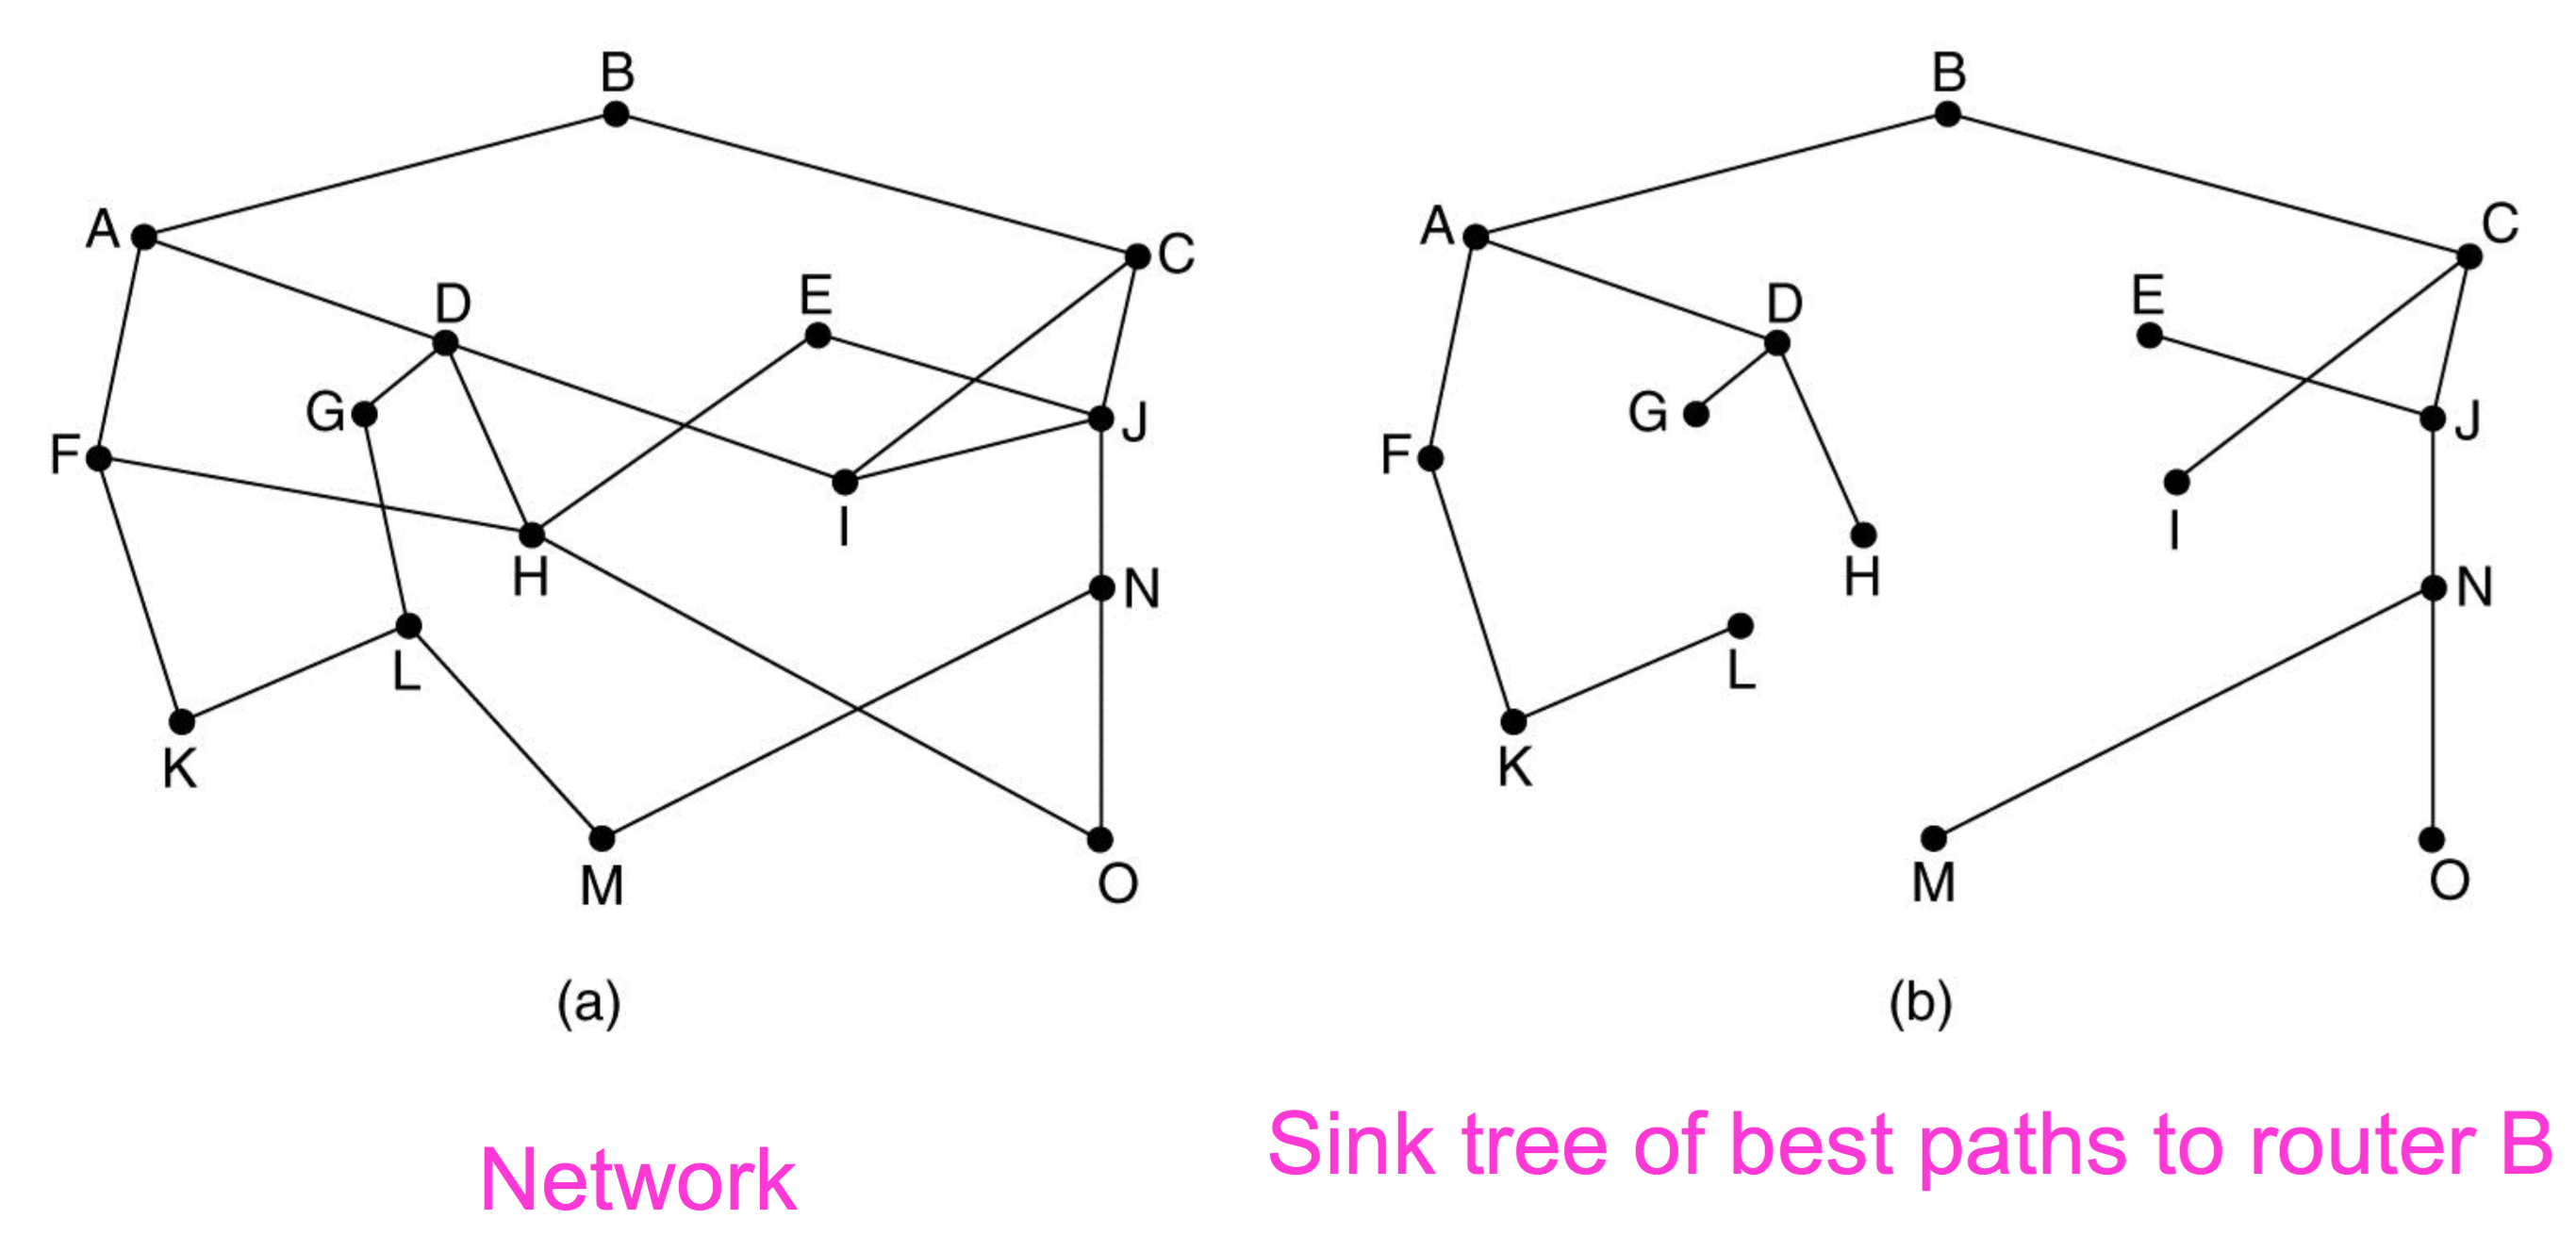
\includegraphics[width=10cm, height=6cm]{./imagenes/optimalidad.png}
	\end{center}

	\par Por ende la meta de todos los algoritmos de enrutamiento es descubrir y utilizar 
	los árboles sumideros de todos los enrutadores.
	
	\par Comenzaremos estudiando algoritmos estáticos, los mismos no son muy 
	buenos, pero veremos que pequeñas variantes de ellos son usados por los algoritmos 
	adaptivos.

\subsection{Algoritmo de la ruta más corta}
	\par La idea es construir un grafo de la red, en donde cada nodo del grafo 
	representa un enrutador y cada arco del grafo representa una línea o enlace de 
	comunicaciones. Para elegir una ruta entre un par específico de enrutadores, el 
	algoritmo simplemente encuentra la ruta más corta entre ellos en el grafo.

	\par Una manera de medir la longitud de una ruta es mediante el número de saltos. 
	Otra métrica es la distancia geográfica en kilómetros, etc. En el caso más general, las 
	etiquetas de los arcos podrían calcularse como función de la distancia, ancho de 
	banda, tráfico medio, costo de comunicación, longitud media de las colas, retardo 
	medio, y otros factores.

	\par Se conocen varios algoritmos para calcular la ruta más corta entre dos nodos de 
	un grafo. Uno de éstos se debe a Dijkstra.


	\par \textbf{Algoritmo de Dijktra:}
		\begin{itemize}
			\item Calculamos la ruta más corta posible entre \emph{s} y \emph{t}
			comenzando por el nodo de destino \emph{t}.
			\item El algoritmo calcula un árbol sumidero en la subred.
			\item Cada nodo se etiqueta con su distancia al nodo de origen a través de la 	
			mejor ruta conocida (al comienzo todos los nodos tienen etiqueta <). Mientras 
			avanza el algoritmo las etiquetas pueden cambiar reflejando mejores rutas.
 			\item Una etiqueta puede ser tentativa o permanente. Inicialmente todas las 
 			etiquetas son tentativas. Cuando se descubre que una etiqueta representa la 
 			ruta más corta del origen a ese nodo, se vuelve permanente y no cambia más.
			\item Se tiene una iteración para la cua lsiempre hay un nodo de trabajo. Ese 
			nodo de trabajo es el nodo tentativo con la menor etiqueta calculado en el paso 
			de iteración anterior (Inicialmente el nodo de trabajo es \emph{t}).
			
			En cada paso de la iteración se actualizan las etiquetas de los nodos tentativos 
			siempre y cuando el nodo de trabajo ayude a encontrar una ruta mejor.
		\end{itemize}

	\begin{center}
	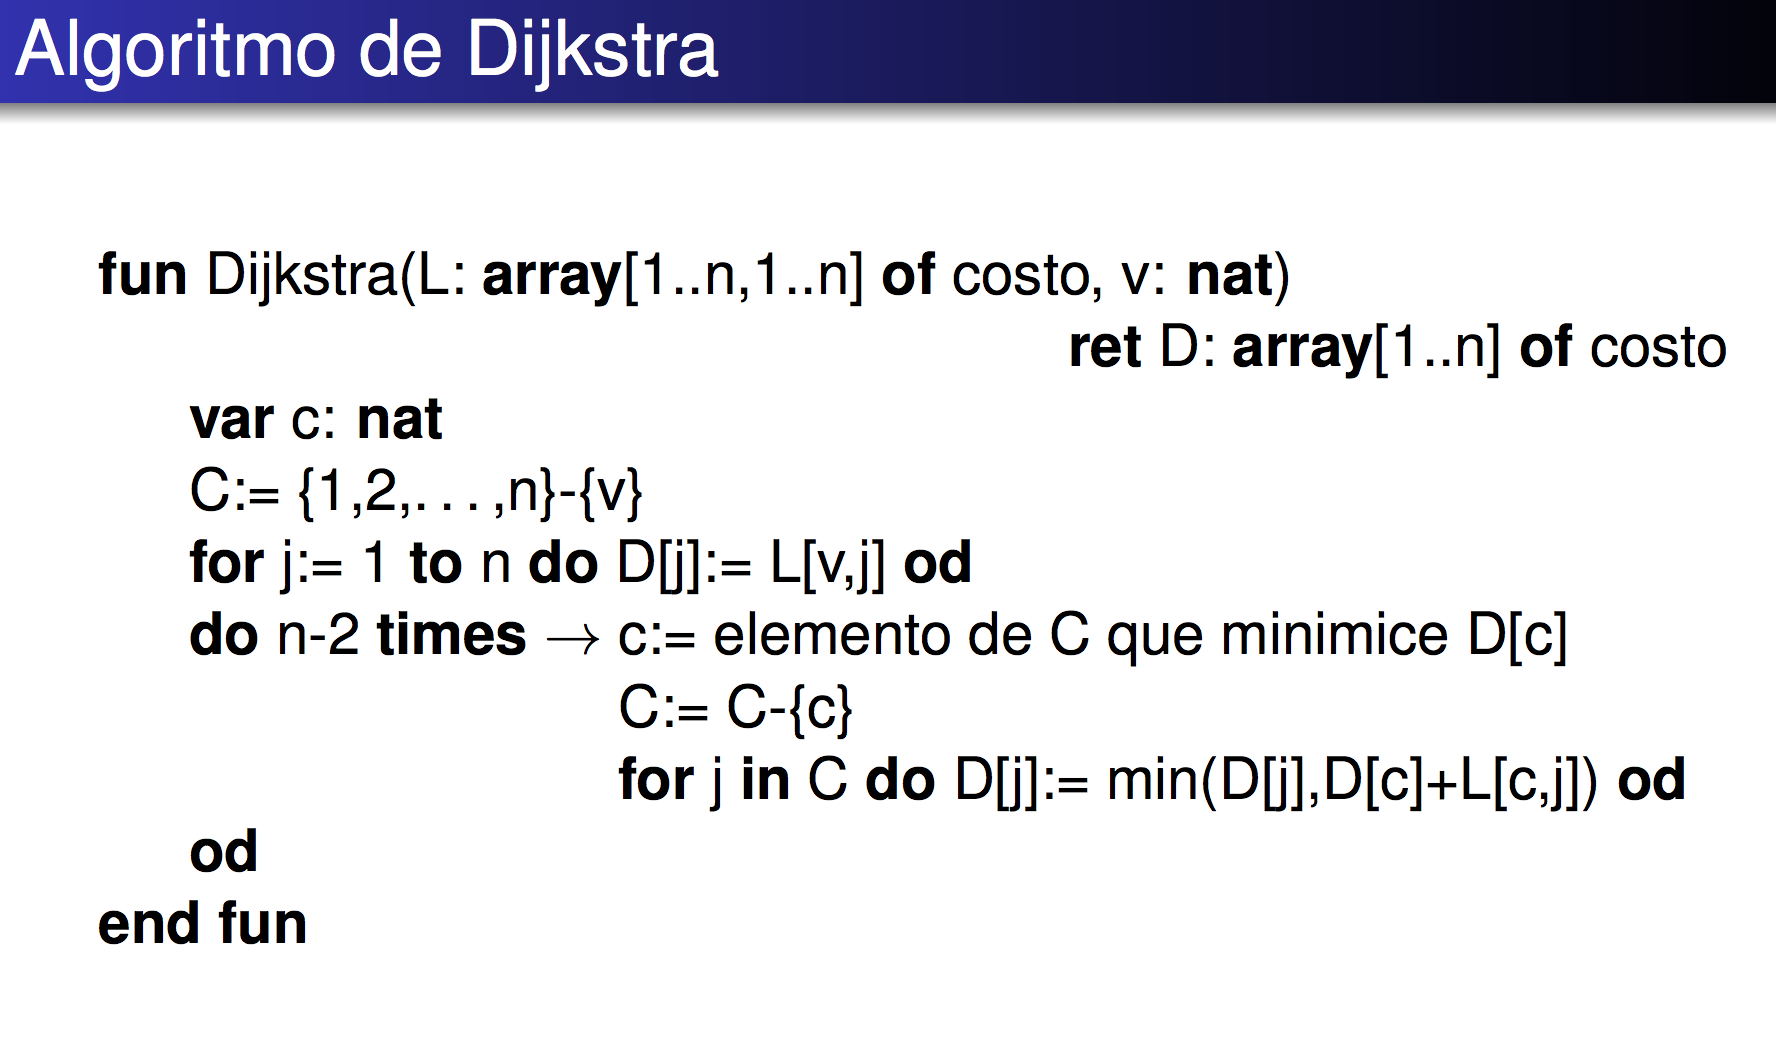
\includegraphics[width=8cm, height=5cm]{./imagenes/dijktra.png} 

	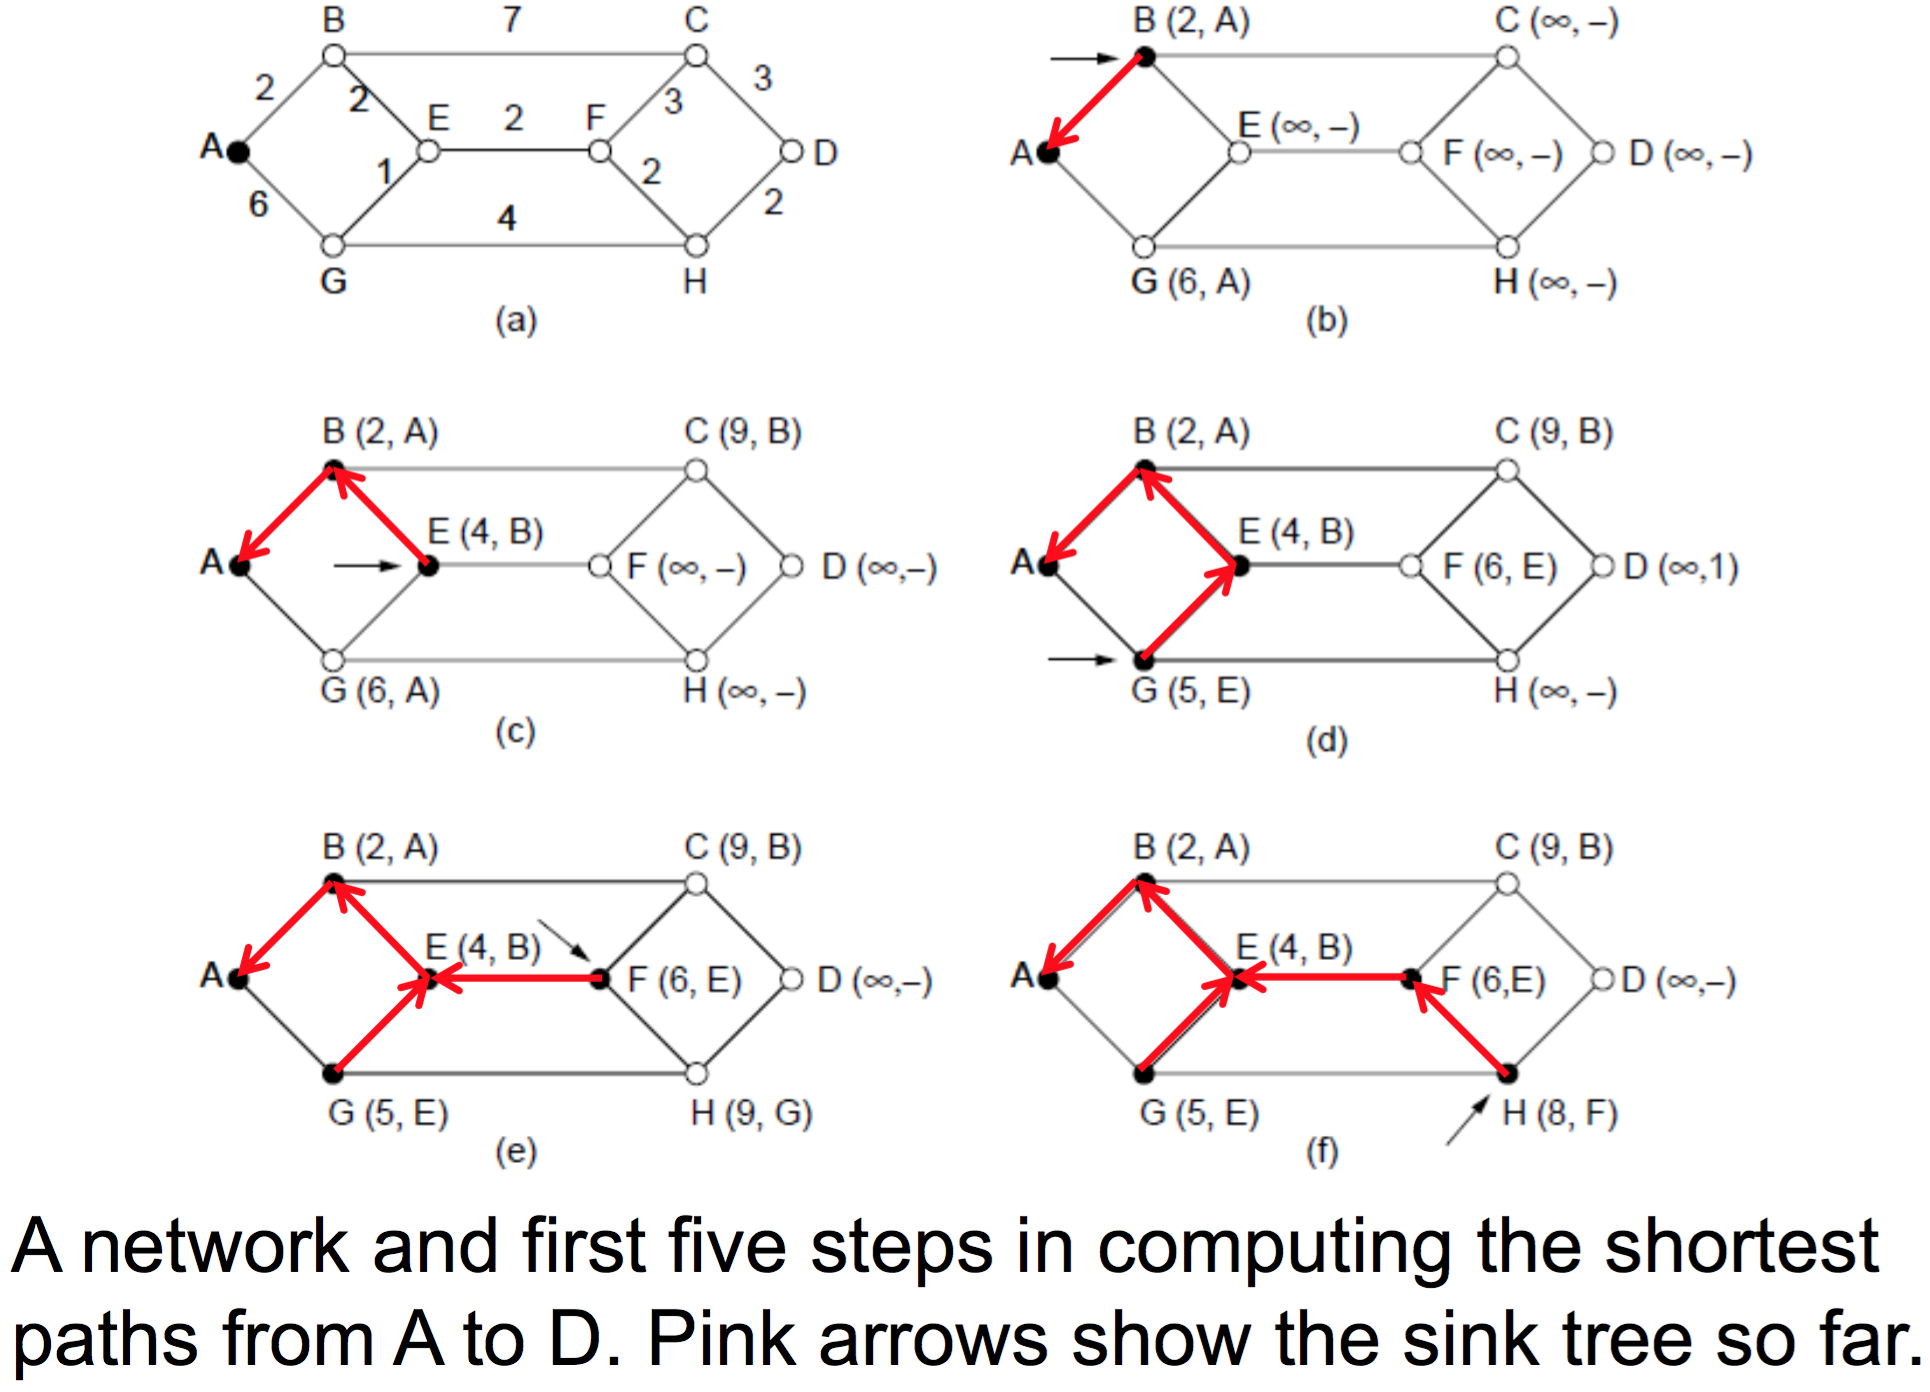
\includegraphics[width=10cm, height=6cm]{./imagenes/caminos.png}
	\end{center}

\subsection{Inundación}
	\par Otro algoritmo estático es la inundación, en la que cada paquete de entrada se 
	envía por cada una de las líneas de salida, excepto aquella por la que llegó.
    Esta idea tiene un problema, la inundación genera grandes cantidades de paquetes 
    duplicados; a menos que se tomen algunas medidas para limitar el proceso. Veamos 
    algos de estas ideas:

	\begin{itemize}
		\item \underline{Solución 1:} integrar un contador de saltos en el encabezado de cada 
		paquete, que disminuya con cada salto y el paquete se descarte cuando el 
		contador llega a 0. Lo ideal es inicializar el contador de saltos a la longitud de la 
		ruta entre el origen y el destino. Si el emisor desconoce el tamaño de la ruta, 
		puede inicializar el contador al peor caso, es decir, al diámetro total de la subred.
		
		\item \underline{Solución 2:} llevar un registro de los paquetes difundidos para evitar 
		enviarlos por segunda vez. Hacer que el enrutador de origen ponga un número de 
		secuencia en cada paquete que recibe de sus hosts. Para cada enrutador de origen 
		hay una lista con los números de secuencia originados en ese enrutador que ya ha 
		visto. Si un paquete de entrada está en la lista, no se difunde.

		\par Para evitar que las listas crezcan sin límites podemos agregar una columna 
		contador que indica el mayor número de secuencia tal que llegaron paquetes con 
		todos los numeros de secuencia anteriores desde ese enrutador de origen.
		
		\item \underline{Solución 3:} Una variación de la inundación, un poco mas práctica, es la 
		inundación selectiva. Los enrutadores no envían cada paquete de entrada por 
		todas las líneas, sino solo por aquellas que van aproximadamente en la dirección 
		correcta.

		\par A nivel de información, se necesita saber en qué  dirección va cada línea y en qué 
		dirección está el destino.
		
		\par La inundación no es práctica en la mayoría de las aplicaciones, pero tiene
		algunos usos, por ejemplo, en aplicaciones militares, en aplicaciones distribuidas 
		de bases de datos. La inundación siempre elige la ruta más corta posible porque 
		escoge en paralelo todas las rutas posibles. En consecuencia ningún otro 
		algoritmo puede producir un retardo más corto (si ignoramos la sobrecarga 
		generada por el proceso de inundación mismo).
		
	\end{itemize}
		
\subsection{Enrutamiento por vector de distancia}

	\par 	Existen dos algoritmos dinámicos que son los más populares: el enrutamiento 
	por vector de distancia y el enrutamiento por estado del enlace. En esta sección 
	veremos el primer algoritmo, en la siguiente estudiaremos el segundo.
	\par En el enrutamiento por vector de distancia, cada enrutador mantiene una tabla 
	de enrutamiento indizada por cada enrutador de la red. Esta entrada consta de dos 
	partes:
	\begin{itemize}
			\item La línea preferida de salida a usar para ese destino
			\item Una estimación del tiempo o distancia a ese destino. 
	\end{itemize}
	\par La distancia se podría medir como la cantidad de saltos, o se podría usar otra 
	métrica, como vimos al calcular las rutas más cortas. 
	\par 	Estas tablas se actualizan intercambiando información con los vecinos. Este 
	algoritmo se usó en Internet con el nombre \textbf{RIP}.
	
	\par Se supone que el enrutador conoce la “distancia” a cada uno de sus vecinos.
		\begin{itemize}
			\item Si la métrica es de saltos, la distancia es un salto.
			\item Si la métrica es la longitud de la cola, el enrutador simplemente examina 
			cada cola.
			\item Si la métrica es el retardo, el enrutador puede medirlo con paquetes de 
			ECO que el receptor simplemente marca con la hora y los regresa tan rápido 
			como puede.
		\end{itemize}
		
	\par Suponga que el retardo se usa como métrica y que el enrutador conoce el 
	retardo a cada uno de sus vecinos. Una vez cada \textit{T} mseg, cada enrutador 
	envía a todos sus vecinos una lista de sus retardos estimados a cada destino.
	También recibe una lista similar de cada vecino. Imagine que la tabla
	\textit{$T_{x}$} acaba de llegar del vecino \textit{X}, en donde \textit{$X_{i}$} es 
	la 	estimación respecto al tiempo que le toma llegar al enrutador \textit{i}. Si el 	
	enrutador sabe que 	el retardo a 	\textit{X} es de \textit{$m_{x}$} mseg, también 
	sabe que puede llegar al enrutador \textit{i} a través de \textit{X} en 
	\textit{$X_{i}$} $+$ \textit{$m_{i}$} mseg. Al efectuar este cálculo para cada 
	vecino, un enrutador puede encontrar la estimación que parezca ser la mejor y usar 
	esa estimación, así como el enlace correspondiente, en su \textbf{nueva tabla de 
	enrutamiento}. Cabe mencionar que en este cálculo no se utiliza la antigua tabla de 
	enrutamiento.

	\par El enrutamiento por vector reacciona con rapidez a las buenas noticias, pero 
	con lentitud ante las malas. Considere un enrutador cuya mejor ruta al destino 
	\textit{X} es larga. Si en el siguiente intercambio el vecino \textit{A} informa 
	repentinamente un retardo corto a \textit{X}, el enrutador simplemente se conmuta 
	a modo de usar la línea a A para enviar tráfico hasta X.
Supongamos que la métrica de retardo es el numero de saltos.
 Las buenas noticias se difunden a razón de un salto por intercambio.
 En una subred cuya ruta mayor tiene una longitud de N saltos, en un lapso de N intercambios todo el mundo sabrá sobre las líneas y enrutadores recientemente revividos.
La razón de porque las malas noticias viajan con lentitud es: ningún enrutador jamás tiene un valor mayor en más de una unidad que el mínimo de todos sus vecinos.
Gradualmente todos los enrutadores elevan cuentas hacia el infinito, pero el número de intercambios requeridos depende del valor numérico usado para el infinito.
Si la métrica usada es el número de saltos, es prudente hacer que el infinito sea igual a la ruta más larga más 1.

	\par Si la métrica es el retardo de tiempo no hay un límite superior
bien definido,
se necesita un valor alto para evitar que una ruta con un retardo grande sea tratada como si estuviera desactivada.
Este es el problema de la cuenta hasta el infinito.
Se han hecho varios intentos para resolverlo, pero ninguno funciona bien
en general.
La esencia del problema consiste en que cuando X indica Xi a E, E no tiene forma de saber si el destino i está en alguna ruta en funcionamiento.

\subsection{Enrutamiento por estado del enlace}
	
	\par La idea detrás del enrutamiento por estado del enlace es bastante simple y 
	se puede enunciar en cinco partes. Cada enrutador debe realizar lo siguiente para 
	hacerlo funcionar:

	\begin{enumerate}
		\item \underline{Descubrir a sus vecinos y conocer sus direcciones de red:} esto lo realiza enviando un paquete HELLO especial a cada línea punto a punto. Se espera que el 	enrutador del otro extremo regrese una respuesta indicando quién es. Estos nombres deben ser globalmente únicos.

		\item \underline{Establecer la métrica de distancia o de costo para cada uno de sus vecinos:} el AEEE requiere que cada enrutador tenga una idea razonable del retardo a cada uno de sus vecinos. Una forma de determinarlo es enviar un paquete ECHO especial a través de la línea, una vez que llegue al otro extremo, éste debe regresarlo inmediatamente.

		\par Si se mide el tiempo de ida y vuelta y se divide por $2$, el enrutador emisor 
		puede tener una idea razonable del retardo. Pero esto tiene un problema, ya que 
		el algoritmo asume de manera implícita que los retardos son simétricos, lo cual no 
		siempre es el caso.

		\par Un aspecto importante es si se debe tener en cuenta la carga al medir el 
		retardo. Para considerar la carga, el temporizador debe iniciarse cuando el paquete 
		ECHO se ponga en la cola. Para ignorar la carga, el temporizador debe iniciarse 
		cuando el paquete ECHO alcance el frente de la cola.
		
		\par Cuando un enrutador puede escoger entre dos líneas con el mismo ancho de 
		banda, una con carga alta continua y otra sin ella, considerará como ruta más 
		corta la de la línea sin carga. Esta selección resultará en un mejor desempeño. 		
		Desgraciadamente también hay un argumento en contra de la inclusión de la carga 
		en el cálculo del retardo.

		\item \underline{Construir un paquete que indique todo lo que acaba de aprender:} Cada enrutador construye un \textbf{paquete de estado} de enlace (LSP) que contiene todos los datos:
		\begin{itemize}
			\item Identidad del emisor
			\item Numero de secuencia
			\item Edad
			\item Lista de (vecino, retardo al vecino)
		\end{itemize}
		
		\textbf{Ejemplo:}
		\begin{center}
			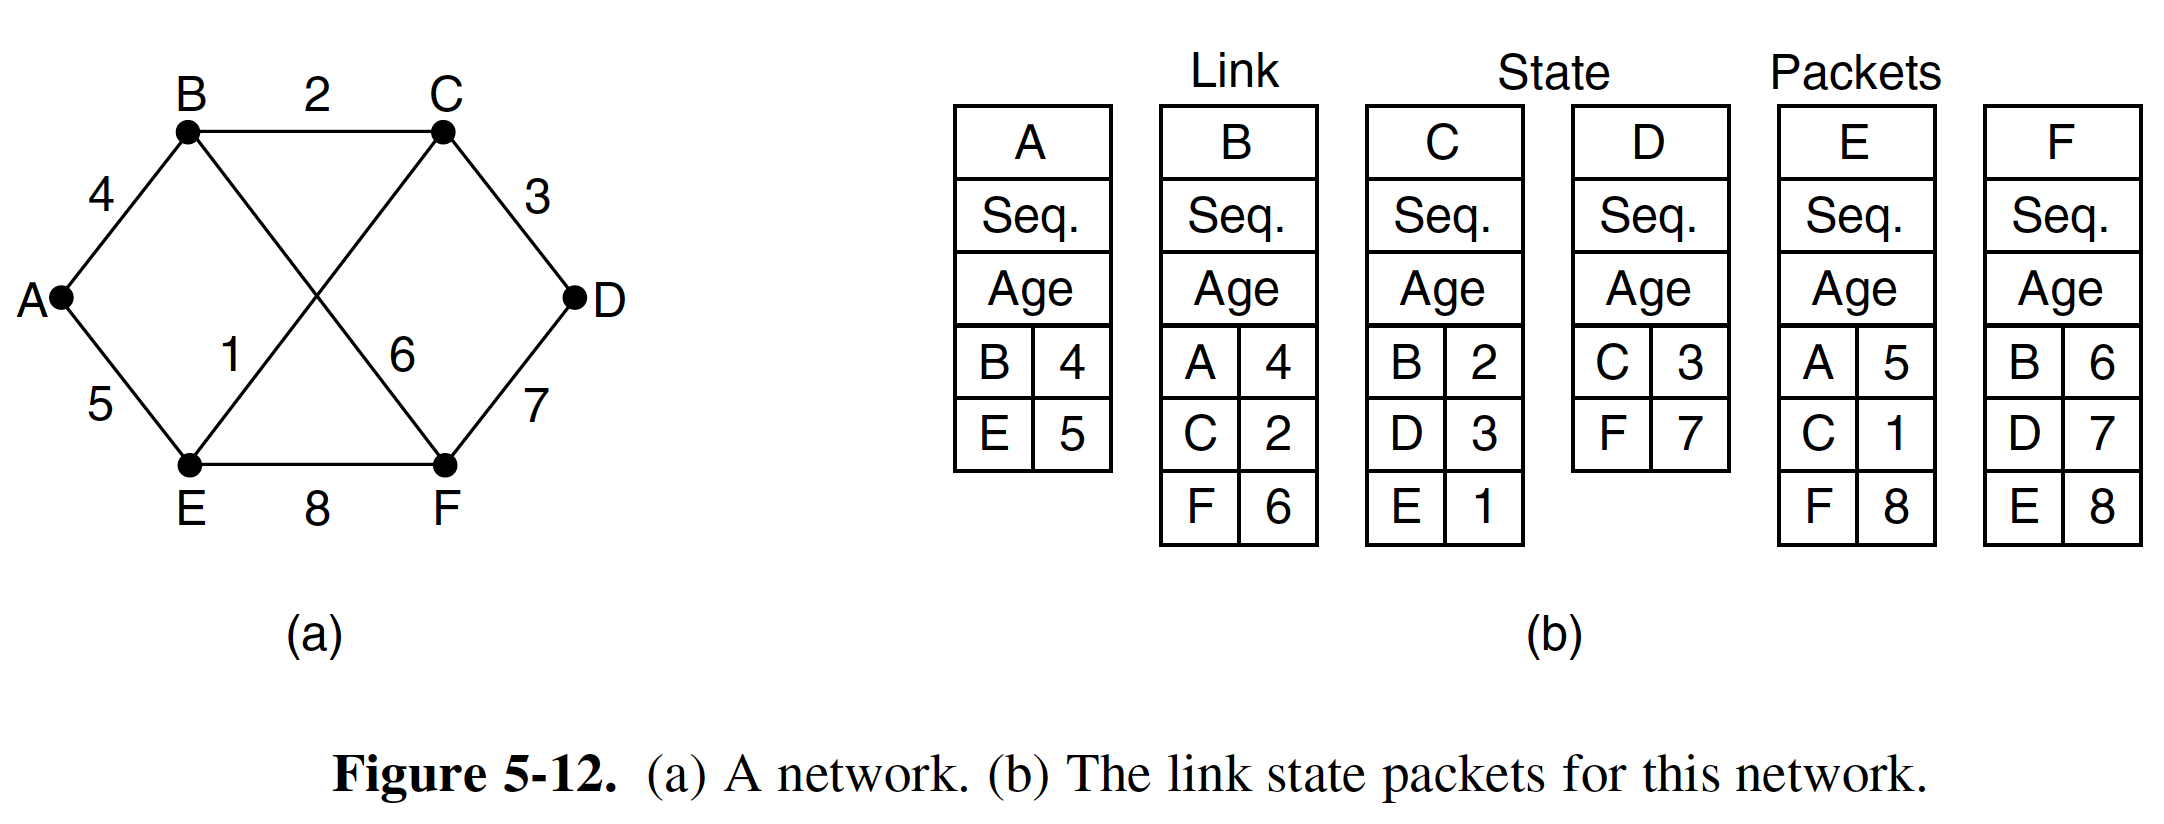
\includegraphics[width=12cm, height=5cm]{./imagenes/estado.png} 
		\end{center}

		\par Los paquetes deben ser construirlos de manera periódica, es decir, a 
		intervalos regulares o cuando ocurra un evento significativo, como la caída o la 
		reactivación de la línea o de un vecino, o el cambio apreciable de sus propiedades.

		\item\underline{ Enviar este paquete a todos los demás enrutadores y recibir paquetes de ellos:} la parte más complicada del algoritmo es la distribución confiable de los  paquetes de estado del enlace.
		
		\par La idea fundamental es utilizar inundación para distribuir los paquetes de estado del enlace a todos los enrutadores. Con el fin de mantener controlada la inundación, cada paquete contiene un número de secuencia que se incrementa con cada nuevo paquete enviado. Los enrutadores llevan el registro de todos los pares (enrutador de origen, secuencia) que ven. Cuando llega un nuevo paquete de estado del enlace, se verifica y compara con la lista de paquetes ya vistos. Si es nuevo, se reenvía a través de todas
las líneas, excepto aquella por la que llegó. Si es un duplicado, se descarta. Si llega un paquete con número de secuencia menor que el mayor visto hasta el momento, se rechaza como obsoleto debido a que el enrutador tiene datos más recientes.

		\par Este algoritmo tiene algunos problemas, pero son manejables. Primero, si los números de secuencia vuelven a comenzar, reinará la confusión. La solución aquí es utilizar un número de secuencia de 32 bits. Con un paquete de estado del enlace por segundo, el tiempo para volver a empezar será de 137 años, por lo que podemos ignorar esta posibilidad.

		\par Segundo, si llega a fallar un enrutador, perderá el registro de su número de secuencia. Si comienza nuevamente en 0, se rechazará como duplicado el siguiente paquete que envíe. Cuando se actualicen las tablas de enrutamiento y se manden los paquetes HELLO, se puede detectar que el enrutador está caído.

		\par Tercero, si llega a corromperse un número de secuencia y se recibe 65540 en vez de 4 (un error de 1 bit), los paquetes 5 a 65540 se rechazarán como obsoletos, dado que se piensa que el número de secuencia actual es 65540.
		
		\par La solución a todos estos problemas es incluir la edad de cada paquete después del número de secuencia y disminuirla una vez cada segundo. Cuando la edad llega a cero, se descarta la información de ese enrutador.

		\par Algunos refinamientos a este algoritmo pueden hacerlo más robusto. Una vez que llega un paquete de estado del enlace a un enrutador para ser inundado, no se encola para su transmisión de inmediato, sino que se coloca en un área de almacenamiento para esperar un tiempo corto, en caso de que se activen o desactiven más enlaces. Si llega otro paquete de estado del enlace proveniente del mismo origen antes de que se transmita el primer paquete, se comparan sus números de secuencia. Si son iguales, se descarta el duplicado. Si son diferentes, se desecha el más antiguo.

		\par El \textbf{buffer de paquetes para un enrutador} contiene una celda por cada paquete de estado de enlace recién llegado, pero aún no procesado por completo. Una fila de la tabla del búfer de paquetes de un enrutador contiene: Origen del paquete, número de secuencia, edad, datos de los estados de enlaces. Banderas que pueden ser:

		\begin{itemize}
			\item \textbf{Banderas de confirmación de recepción:} indica a dónde tiene que enviarse la confirmación de recepción del paquete.
			\item \textbf{Banderas de envío:} significan que el paquete debe enviarse a través de las líneas indicadas.
			\item Si llega un duplicado mientras el original aún esta en el búfer, los bits de las banderas tienen que cambiar.
		\end{itemize}
		
		\begin{center}
			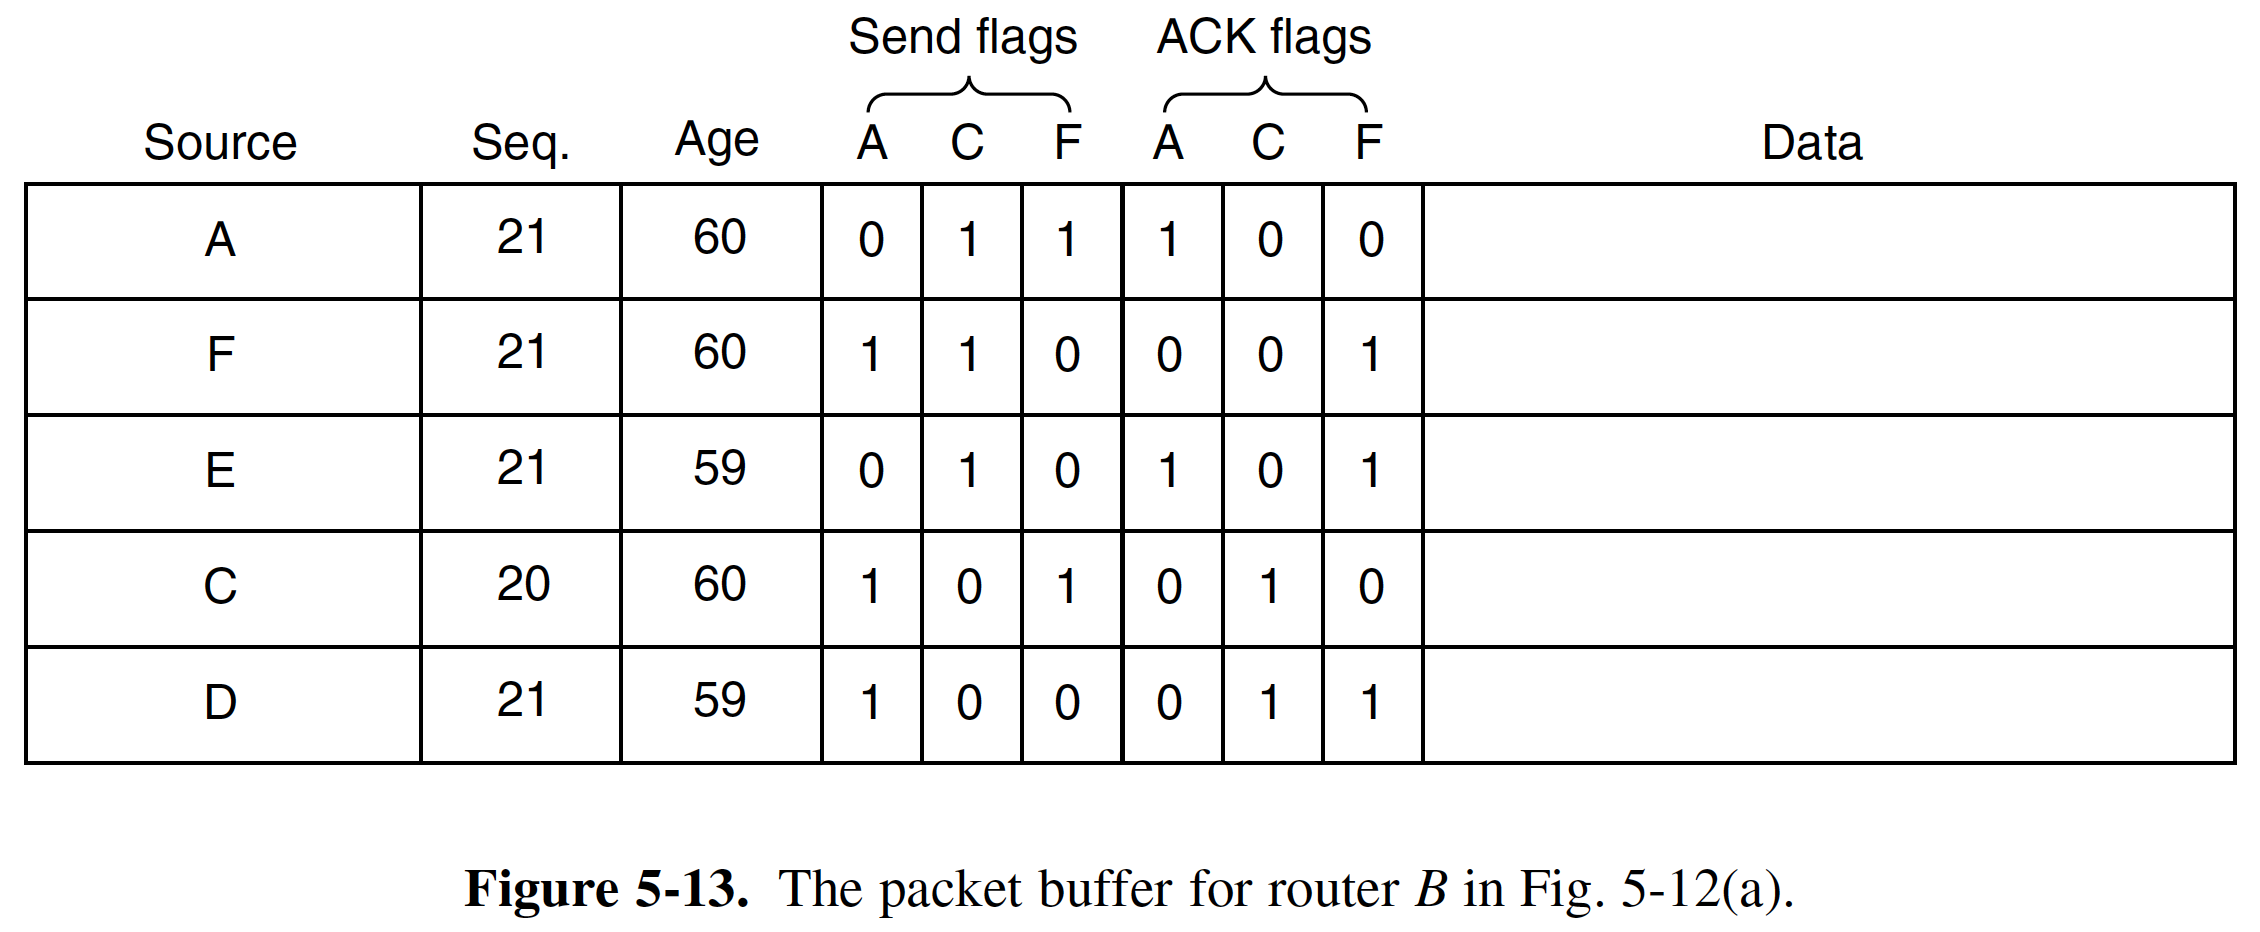
\includegraphics[width=9cm, height=4cm]{./imagenes/eenlace.png} 
		\end{center}

		\item \underline{Calcular la ruta más corta a todos los demás enrutadores:} una vez que el enrutador ha acumulado un grupo completo de paquetes de estado del enlace, puede construir el grafo de la subred completa. Cada enlace se representa dos veces, una para cada dirección. Los dos valores pueden promediarse o usarse por separado. Luego se ejecuta localmente el algoritmo de Dijkstra para construir la ruta más corta a todos los destinos posibles. Los resultados de este algoritmo pueden instalarse en las tablas de enrutamiento, y la operación normal puede reiniciarse.

		\par  A medida que la subred crece en decenas de miles o cientos de miles de nodos, la probabilidad de falla ocasional de un enrutador deja de ser insignificante. El algoritmo por estado de enlace se usa ampliamente en las redes actuales.
	\end{enumerate}

\subsection{Enrutamiento jerárquico}

	\par A medida que crece el tamaño de las redes, también lo hacen en forma proporcional las tablas de enrutamiento del enrutador. Las tablas que están en crecimiento constante no sólo consumen memoria del enrutador, sino que también se necesita más tiempo de CPU para examinarlas y más ancho de banda para enviar informes de estado entre enrutadores. La subred puede crecer hasta el punto en que ya no sea viable que cada enrutador tenga una entrada para cada uno de los demás enrutadores.
	
	\par Cuando se utiliza el enrutamiento jerárquico, los enrutadores se dividen en lo que llamaremos regiones. Cada enrutador conoce todos los detalles para enrutar paquetes a destinos dentro de su propia región, pero no sabe nada de la estructura interna de las otras regiones. 
	
	\par Resolver este problema es necesario porque las WAN suelen ser enormes
y también lo es la internet. Sin resolver este problema solo se podrían tener varias WAN chicas o medianas sin interconectarlas entre sí. El hacerlo permite tener dentro de una WAN enorme, redes enormes para grandes empresas (corporaciones) o instituciones públicas (grandes universidades, gobiernos, etc.) y considerar todas las redes del mundo como una única intered gigante.

	\par En las redes enormes, tal vez no sea suficiente una jerarquía de dos niveles; puede ser necesario agrupar las regiones en clústeres, los clústeres en zonas, las zonas en grupos, etc, hasta que se nos agoten los nombres para clasificarlos.
	
	\par Si el enrutador es jerárquico, en su tabla de enrutamiento hay:
		\begin{itemize}
			\item Entradas para todos los enrutadores locales.
			\item Entradas para las las demás regiones en las que no está el enrutador.
		\end{itemize}
	
	\par El precio que se paga con enrutamiento jerárquico es una longitud de ruta mayor.

	\begin{center}
			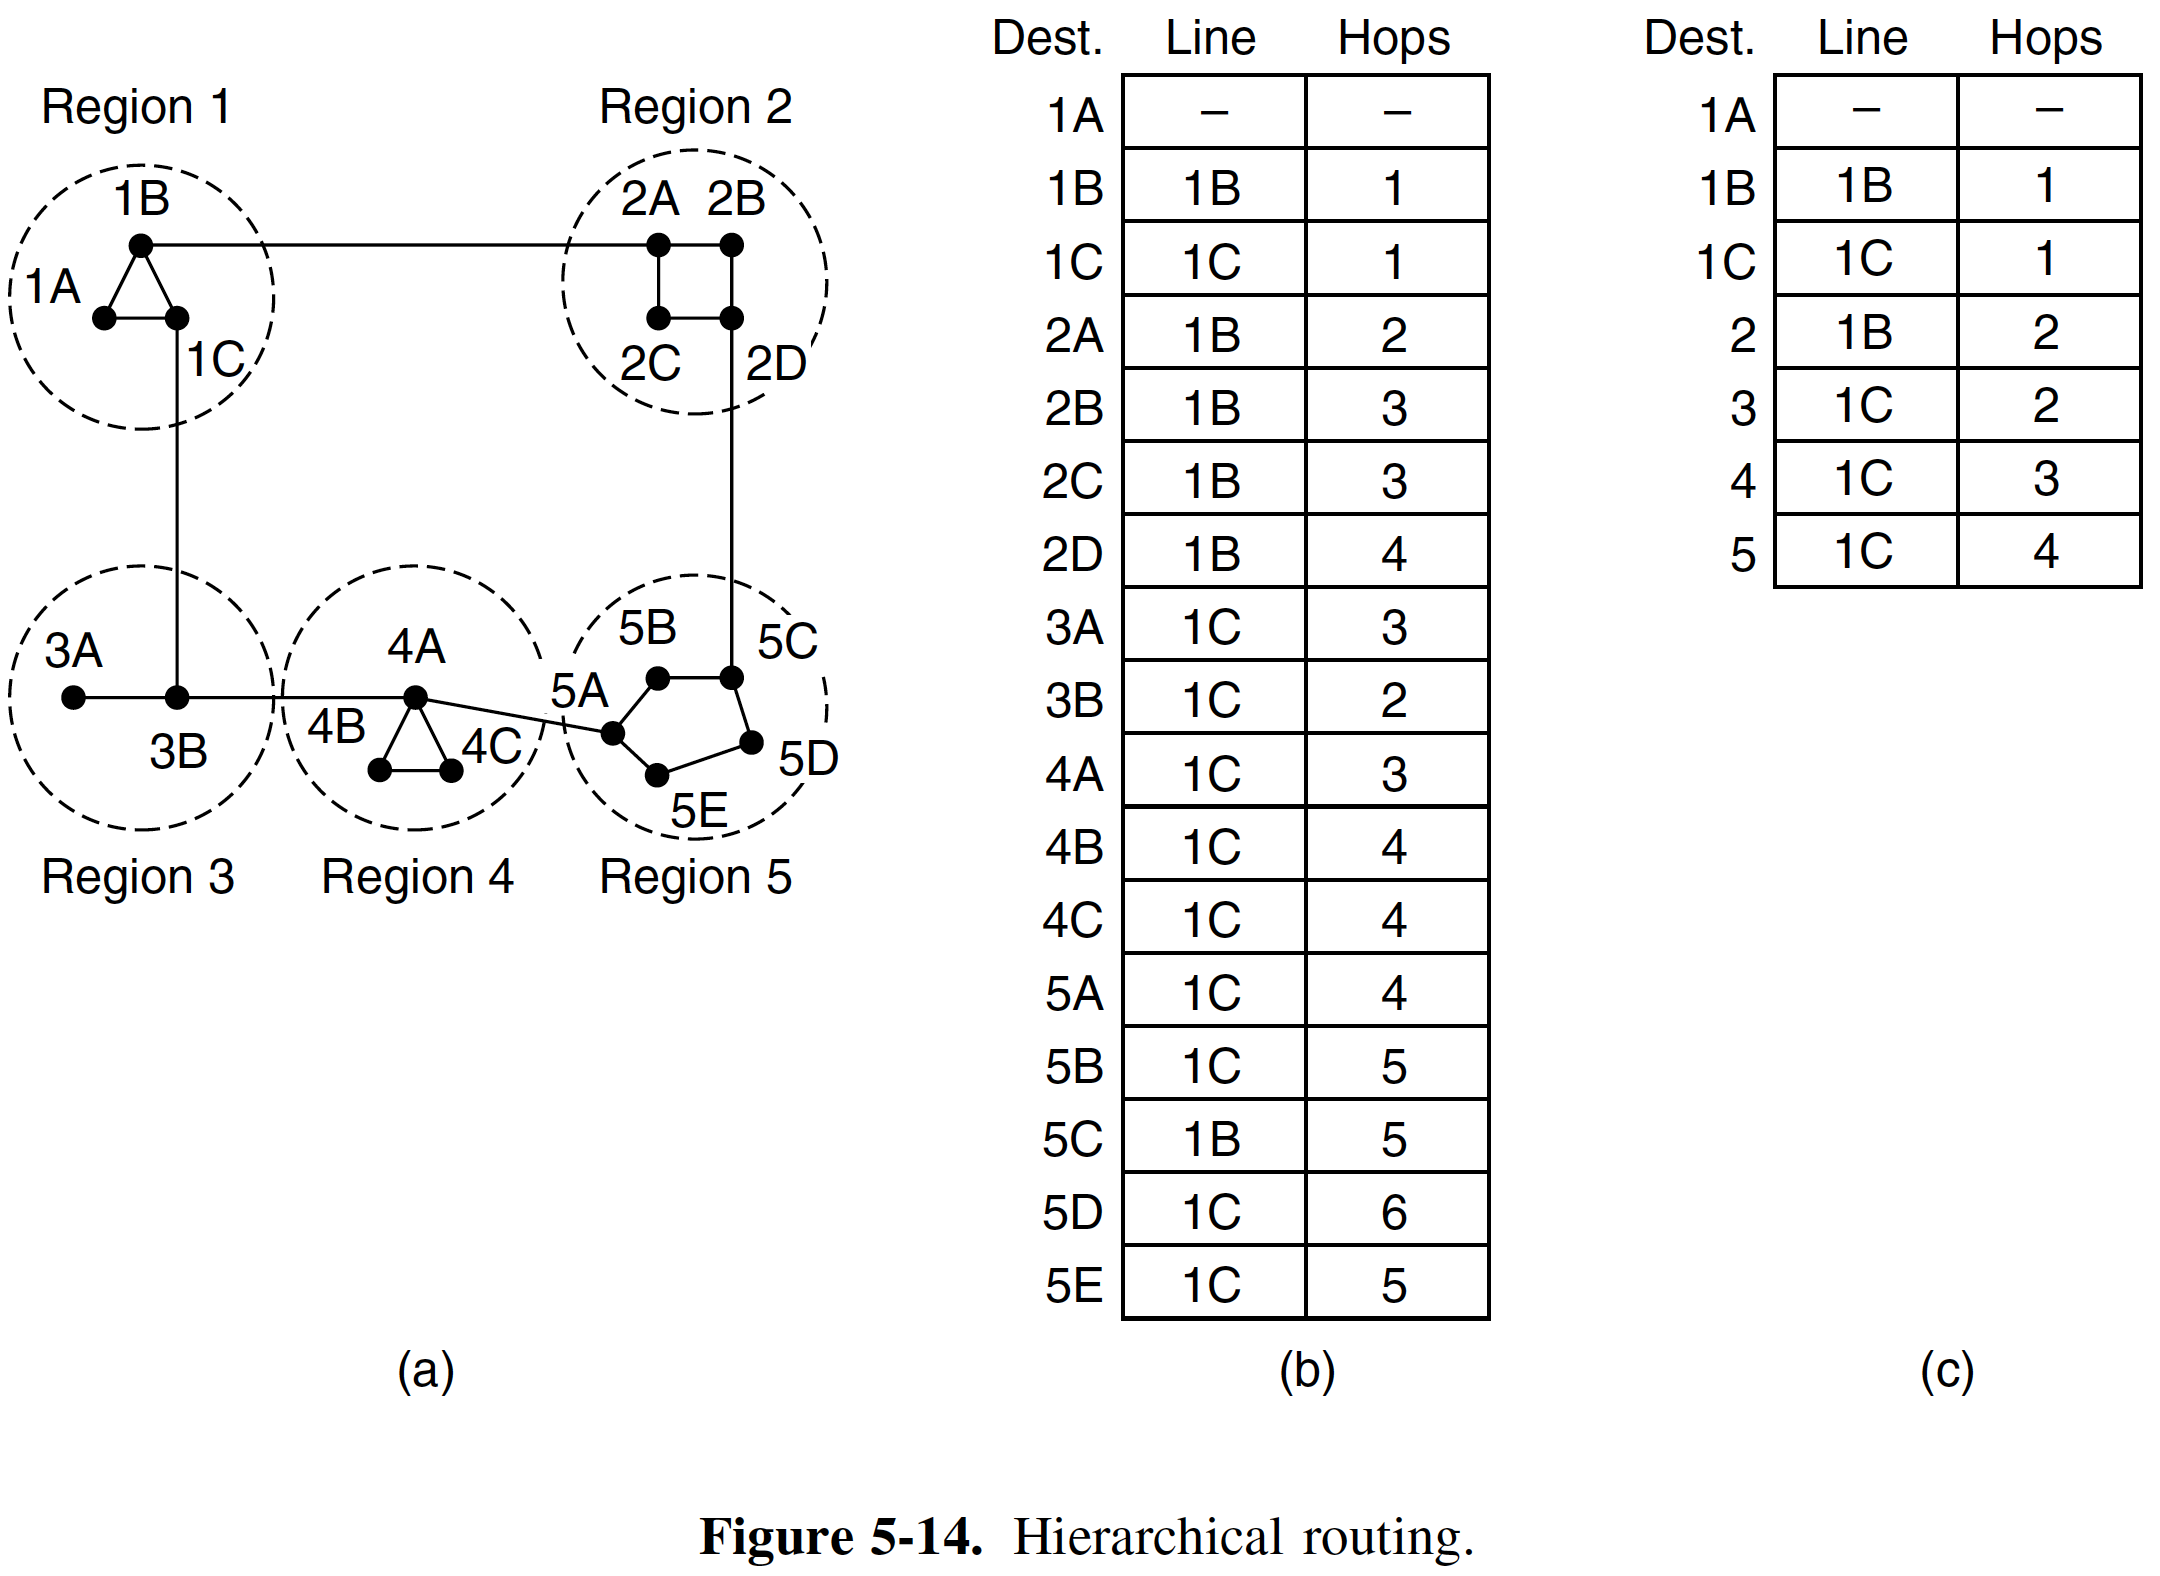
\includegraphics[width=9cm, height=6cm]{./imagenes/jerarquico.png} 
	\end{center}

\section{Algoritmos de control de congestión}

	\par Cuando la cantidad de paquetes descargados en la subred por los \textit{hosts} está dentro de su capacidad de conducción, la cantidad de paquetes entregados es proporcional al número enviado. Cuando hay demasiados paquetes presentes en la subred (o en una parte de ella) hay una degradación del desempeño. Esta situación se llama \textbf{congestión}.

	\par A medida que aumenta el tráfico, llega un punto en que los enrutadores ya no pueden manejarlo y comienzan a perder paquetes. Con mucho tráfico el desempeño se desploma por completo y casi no hay entrega de paquetes.

	\par Si comienzan a llegar muchos paquetes por algunas líneas de entrada y todas necesitan la misma línea de salida. Se generará una cola. Si no hay suficiente memoria para almacenar todos los paquetes, algunos de ellos se perderán.
	
	\begin{center}
			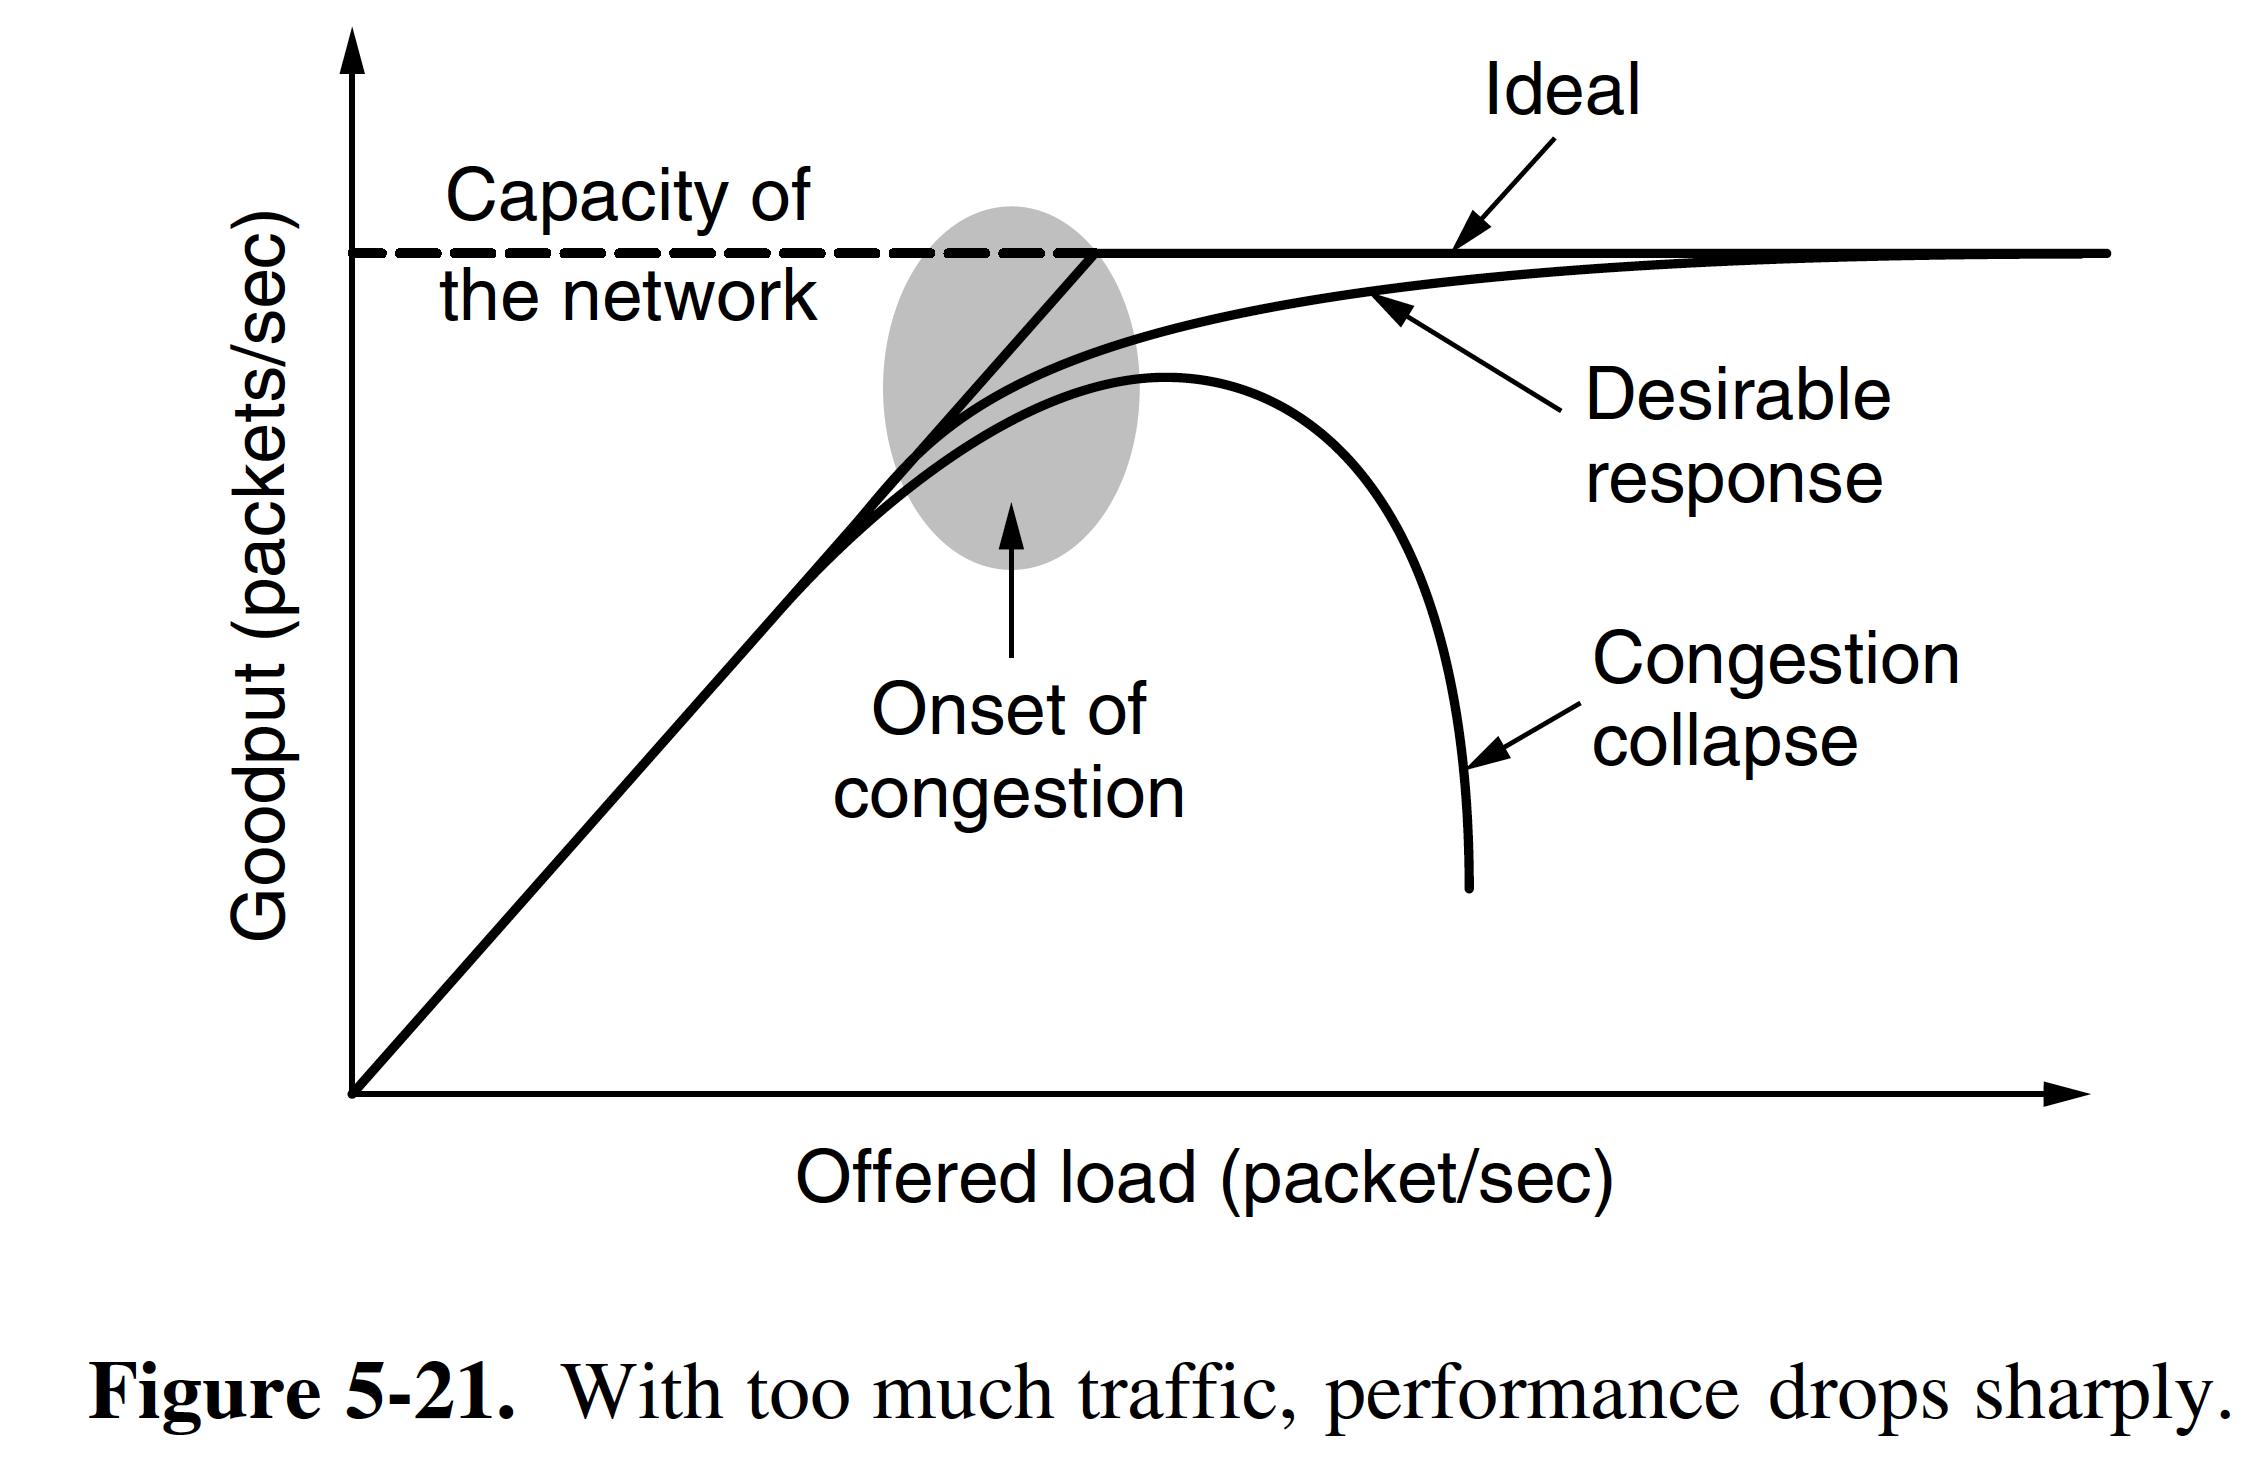
\includegraphics[width=8cm, height=5cm]{./imagenes/congestion.png} 
	\end{center}

	\par El control de congestión se ocupa de asegurar que la subred sea capaz de transportar el tráfico ofrecido. Es un asunto global en el que interviene el comportamiento de todos los hosts, todos los enrutadores, el proceso de almacenamiento y reenvío dentro de los enrutadores y todos los demás factores que tienden a disminuir la capacidad de transporte de la subred.

\subsection{Métodos para el control de la congestión}

	\par La presencia de congestión significa que la carga es (temporalmente) mayor de la que los recursos (en una parte de la red) pueden manejar. Dos soluciones vienen a la mente: aumentar los recursos o reducir la carga.
	
	\par La adición de memoria puede ayudar hasta cierto punto. Se demostró que si los enrutadores tienen infinita memoria, la congestión empeora en lugar de mejorar, ya que para cuando los paquetes llegan al principio de la cola su temporizador ha terminado (repetidamente) y se han enviado duplicados. Todos estos paquetes serán reenviados al siguiente enrutador, aumentando la carga en todo el camino hasta su destino.

	\par Los procesadores lentos también pueden causar congestión. Si las CPUs de los enrutadores son lentas para llevar a cabo las tareas requeridas, las colas pueden alargarse, aun cuando haya un exceso de capacidad de línea. Las líneas de poco ancho de banda también pueden causar congestión. Probablemente la cola de una línea de salida de poco ancho de banda se va a agrandar si otras líneas tienen mayor ancho de banda y están recibiendo muchos paquetes destinados a la línea de salida.

	\par La actualización de las líneas sin cambiar los procesadores o viceversa, por lo general ayuda un poco, pero con frecuencia simplemente solo desplaza el cuello de botella a otra parte. El problema real es un desajuste de las partes del sistema, este problema persistirá hasta que todos los componentes estén en equilibrio.

\subsection{Enrutamiento consciente del tráfico}

	\begin{center}
			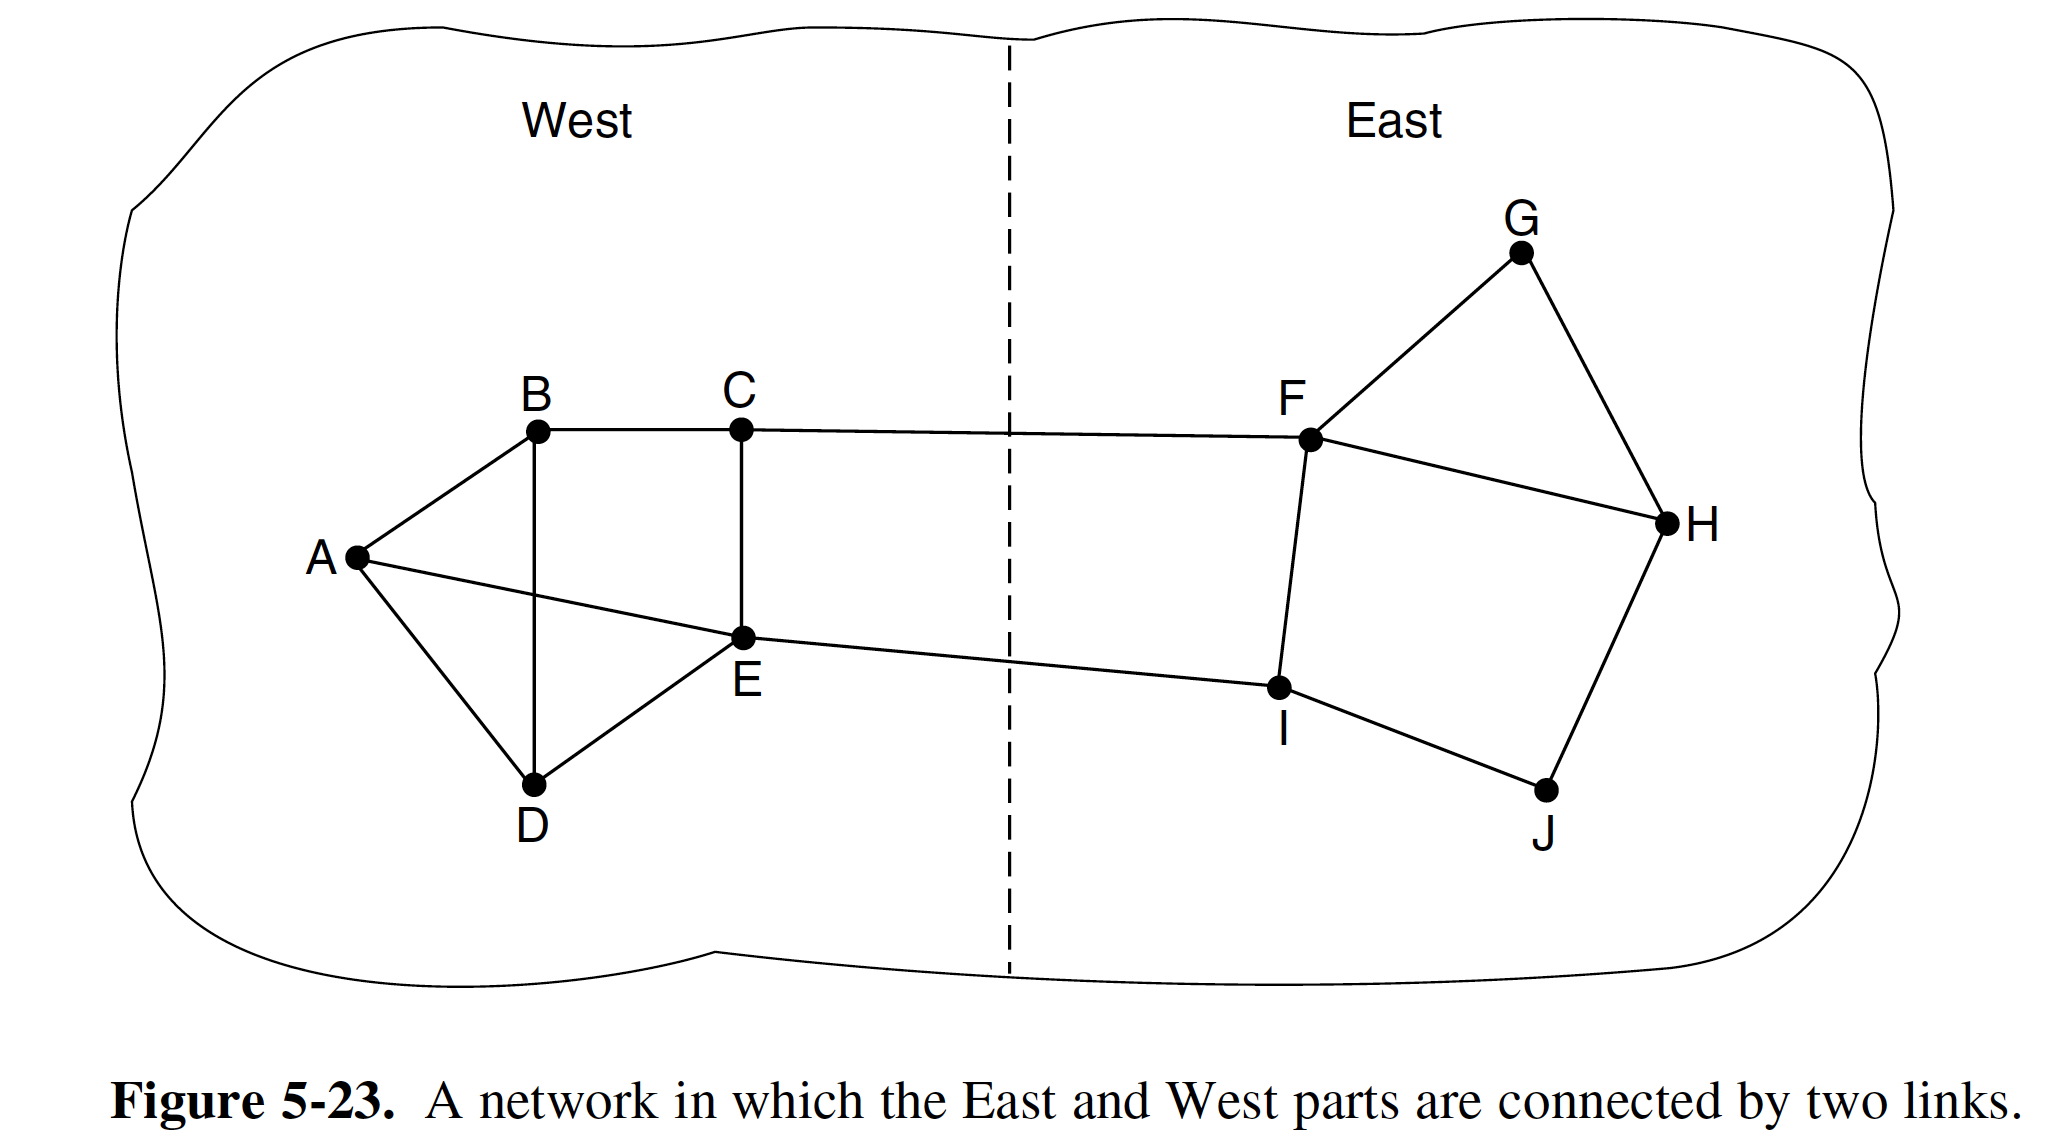
\includegraphics[width=7cm, height=5cm]{./imagenes/consciente.png} 
	\end{center}

\subsection{Control de admisión}

	No se establecen nuevos circuitos Virtuales hasta que desaparece el problema.
	\begin{center}
			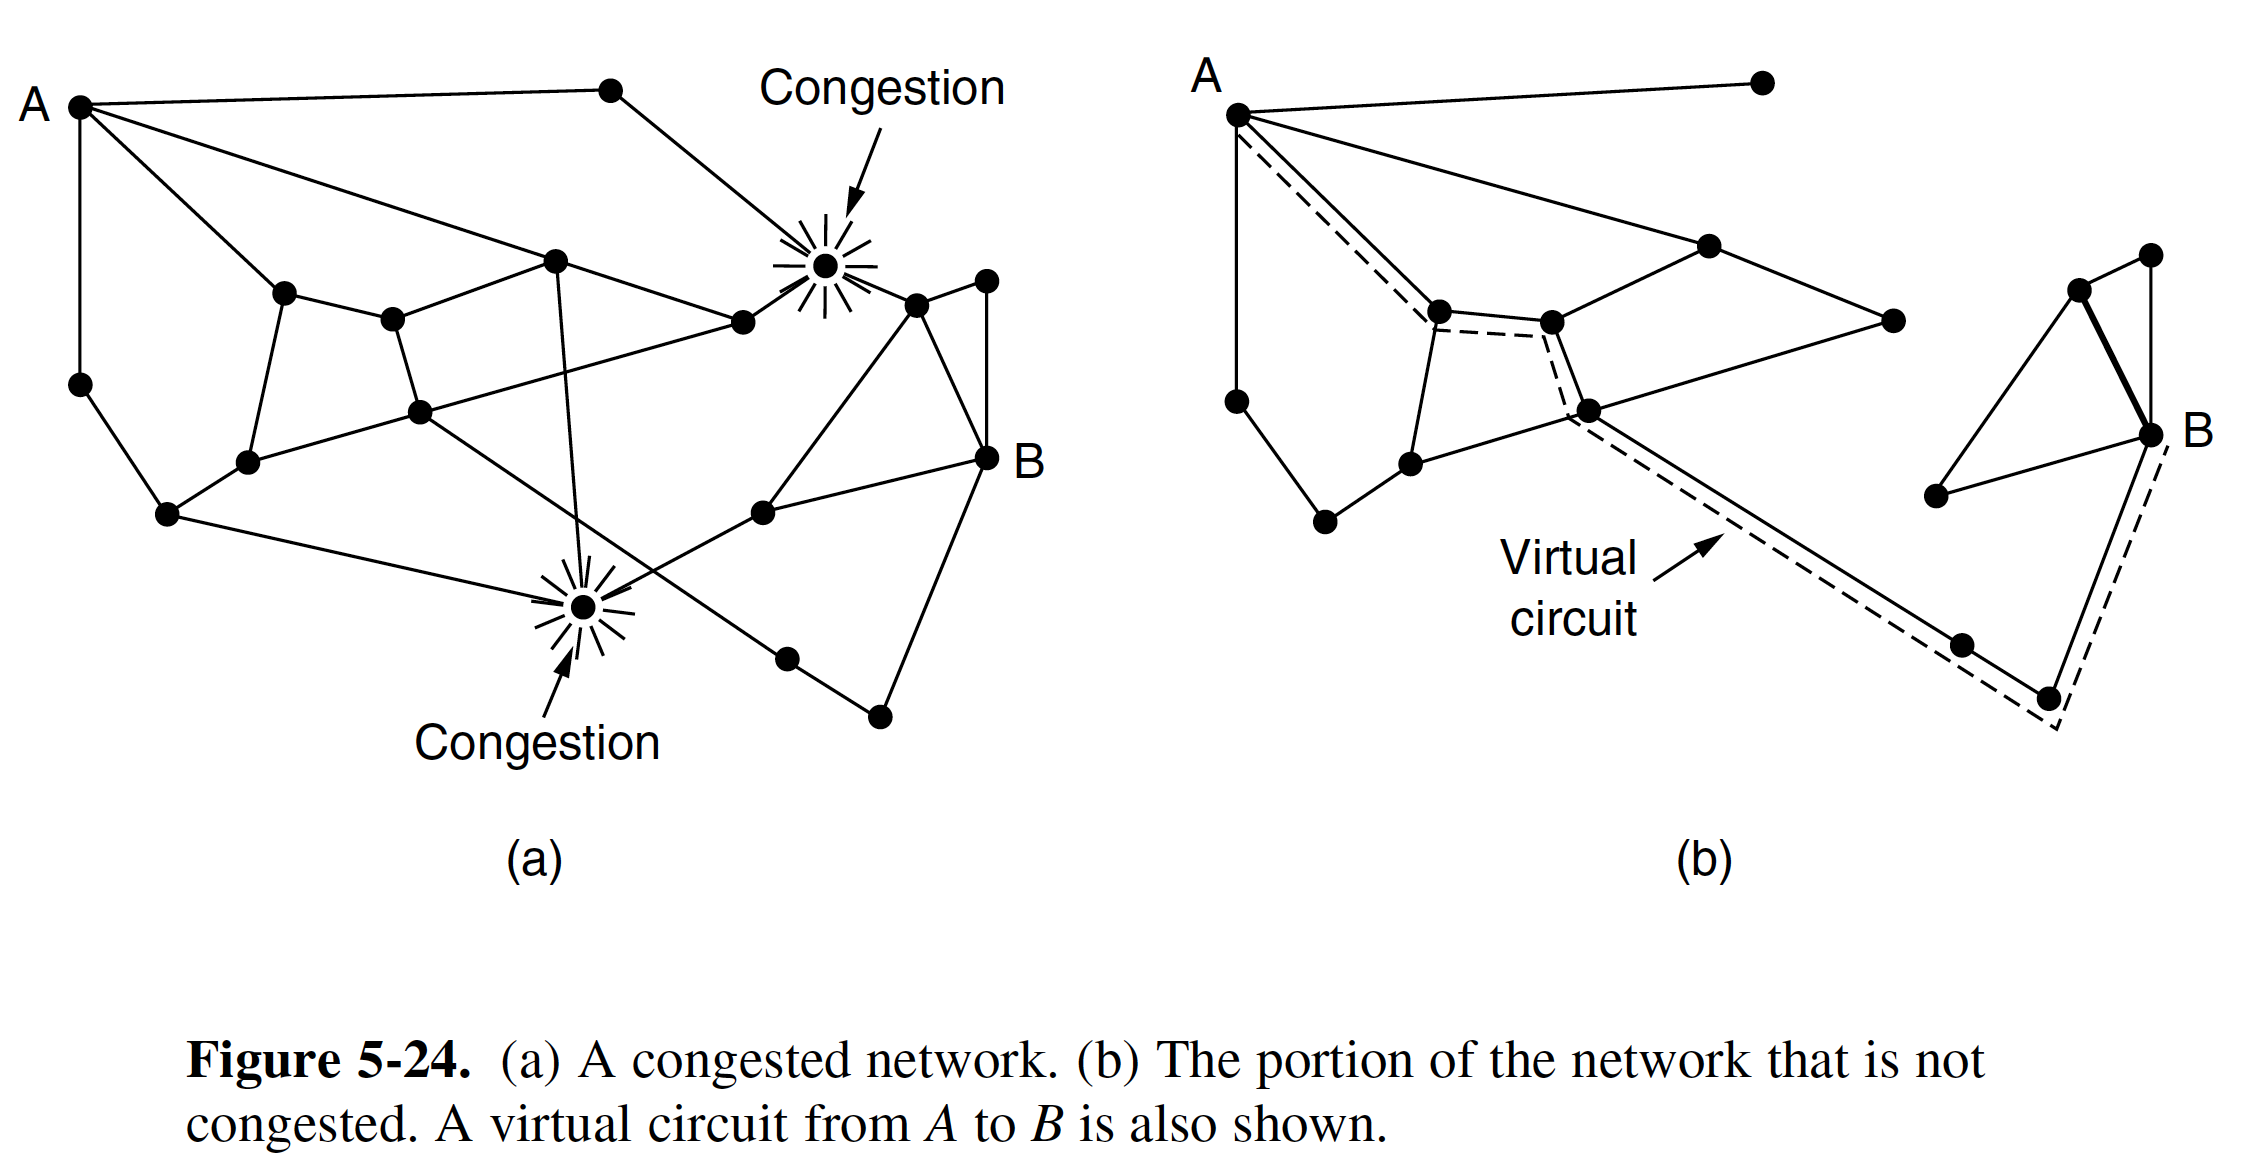
\includegraphics[width=7cm, height=5cm]{./imagenes/admision.png} 
	\end{center}

\subsection{Regulación del tráfico}

	\par El enfoque que vemos ahora puede usarse tanto en subredes de Circuitos Virtuales como en subredes de datagramas. Cada enrutador monitorea la demora de la cola de línea de salida. Para mantener una buena estimación del retardo de encolamiento, \textit{d}, se puede realizar un muestreo periódico de la longitud de cola instantánea, \textit{s}, y se puede actualizar d de acuerdo con:

	\begin{center}
		$ d_{new} = \alpha d_{old} + (1-\alpha) s $
	\end{center}

	\par donde a determina la rapidez con que el enrutador olvida la historia reciente.

	\par Siempre que \textit{d} rebasa el umbral, la línea de salida entra un estado de advertencia. Cada paquete nuevo que llega se revisa para ver si su línea de salida está en el estado de advertencia. Si es así, se realiza alguna acción. Esta puede ser una de varias alternativas que analizaremos a continuación:

	\begin{itemize}
		\item \textbf{Idea 1:} Usar una técnica de control de admisión para evitar que empeoren las congestiones que ya han comenzado y que consiste en que una vez que se ha detectado la congestión, no se establecen CVs nuevos hasta que ha desaparecido el problema.
		\item \textbf{Idea 2:} Permitir el establecimiento de nuevos CV, pero enrutando cuidadosamente los circuitos nuevos por otras rutas que no tengan problemas.

		\item \textbf{Idea 3:} Negociar un acuerdo entre el \textit{host} y la subred cuando se establece un CV. Este arreglo normalmente especifica el volúmen y la forma del tráfico, la calidad de servicio requerido y otros parámetros. Para cumplir con su parte del acuerdo, la subred por lo general reservará recursos a lo largo de la ruta cuando se establezca el circuito. Estos recursos pueden incluir espacio en tablas y en búfer en los enrutadores y ancho de banda en las líneas. De este modo es poco probable que ocurran congestiones en los CV nuevos.
	\end{itemize}

	\par A continuación vemos distintos algoritmos sobre cómo proceder cuando una línea de un enrutador entró en estado de advertencia y le llegó un paquete.

		\begin{itemize}
			\item \textbf{Método de bit de advertencia:} Señalar el estado de advertencia
activando un bit especial en el encabezado del paquete. Cuando el paquete llega a su destino, la entidad transportadora copia el bit en la siguiente confirmación de recepción que se regresa al origen. A continuación el origen reduce el tráfico. Mientras el enrutador está en estado de advertencia, continua activando el bit de advertencia, lo que significa que el origen continua obteniendo confirmaciones de recepción con dicho bit activado.

			\par El origen monitorea la fracción de confirmaciones de recepción con el bit activado y ajusta su tasa de transmisión de manera acorde. En tanto los bits de advertencia continuan fluyendo, el origen continua disminuyendo su tasa de transmisión.

			\par Cuando la tasa de transmisión disminuye lo suficiente, el origen incrementa su tasa de transmisión. Debido a que cada enrutador a lo largo de la ruta puede activar el bit de advertencia, el tráfico se incrementa solo cuando no había enrutadores con problemas.

			\item \textbf{Método de paquetes reguladores.} El enrutador regresa un paquete regulador al \textit{host} de origen, proporcionándole el destino encontrado en el paquete. El paquete original se etiqueta (se activa un bit del encabezado), de manera que no genere más paquetes reguladores más adelante en la ruta y después se reenvía de la manera usual.
	
			\par Cuando el host de origen obtiene el paquete regulador, se le pide que reduzca en un porcentaje X el tráfico enviado al destino especificado. Puesto que otros paquetes dirigidos al mismo destino probablemente ya están en camino y generarán más paquetes reguladores, el \textit{host} debe ignorar los paquetes reguladores que se refieran a ese destino por un intervalo fijo de tiempo. Una vez que haya expirado ese tiempo, el \textit{host} escucha más paquetes reguladores durante otro intervalo. Si llega alguno, la línea todavía está congestionada, por lo que el \textit{host} reduce el flujo aún más y comienza a ignorar nuevamente los paquetes reguladores. Si no llega ningún paquete de este tipo durante el período de escucha, el \textit{host} puede incrementar el flujo otra vez.
 
			\par Manejo de la tasa de datos de transmisión de un host. Por lo general el primer paquete regulador causa que la tasa de datos se reduzca en 0,5 con respecto a su tasa anterior, el siguiente causa una reducción en 0,25, etc. Los incrementos se dan en aumentos más pequeños para evitar que la congestión se vuelva a generar rápidamente.

			\item \textbf{Variación de paquetes reguladores.} Los enrutadores pueden mantener varios umbrales. Dependiendo de qué umbral se ha rebasado, el paquete regulador puede contener una advertencia suave, una severa o un \textit{ultimatum}.
			
			\item \textbf{Método de Paquetes reguladores de salto por salto.} Este método resuelve el problema del envío de paquetes reguladores a los \textit{hosts} de origen que no funcionan bien por la reacción lenta. En este caso hay que hacer que el paquete regulador ejerza su efecto en cada salto que da. Cuando el paquete regulador llega a un enrutador F, se le obliga a F a reducir el flujo al siguiente enrutador D (F deberá destinar más búferes al flujo). Luego el paquete regulador llega al enrutador E anterior a F e indica a E que reduzca el flujo a F. Esto impone una mayor carga a los búferes de E, pero da un alivio inmediato a F. Y se sigue así sucesivamente.
			
			\begin{center}
				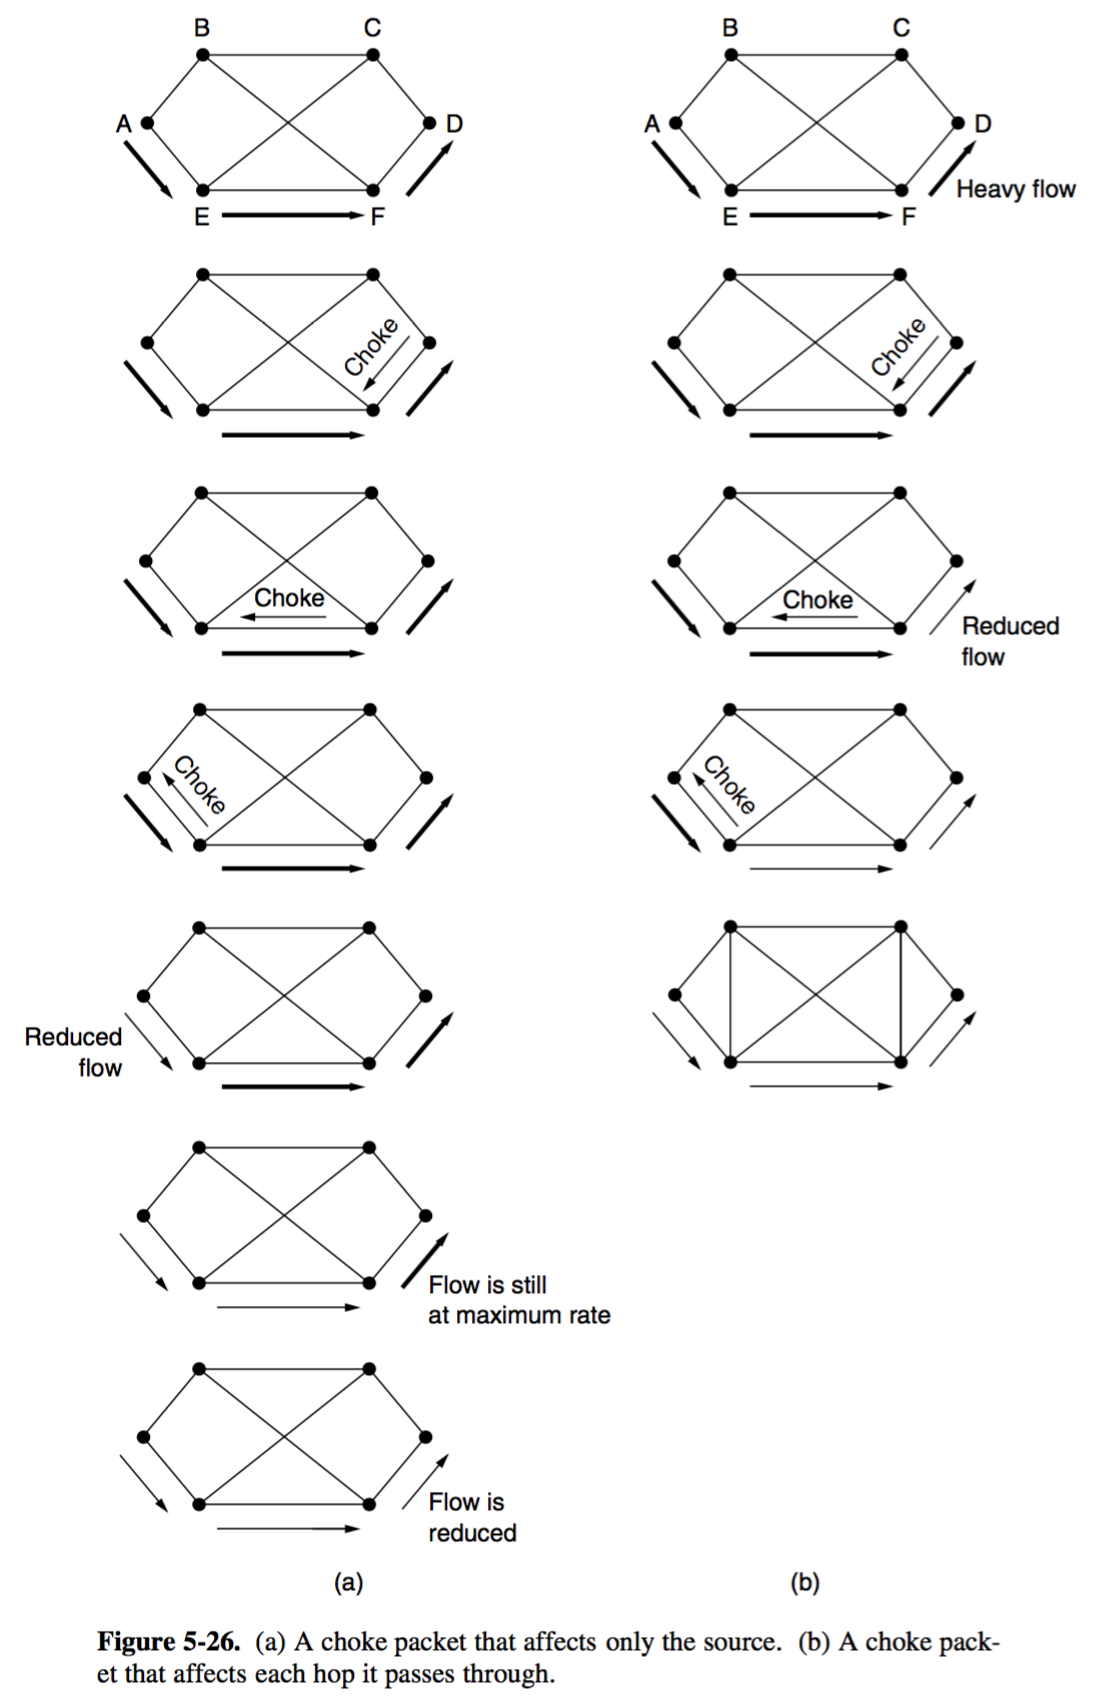
\includegraphics[width=10cm, height=12cm]{./imagenes/salto.png} 
			\end{center}
	
		\end{itemize}

\subsection{Desprendimiento de carga}

	\par Cuando ninguno de los métodos anteriores elimina la congestión, los enrutadores pueden sacar la artillería pesada: el desprendimiento de carga, que es una manera rebuscada de decir que cuando se inunda a los enrutadores con paquetes que no pueden manejar, simplemente se tiran.

	\par Tratar con la congestión después que se detecta por primera vez es más efectivo que dejar que se dañe el trabajo y luego tratar de solucionarlo. Se deben descartar paquetes antes de que se ocupe todo el espacio de búfer. Algunos criterios para escoger qué paquetes descartar:
	
	\begin{itemize}
		\item Según el tipo de aplicación que se está usando.
			\begin{itemize}
				\item En la transferencia de archivos vale más un paquete viejo que uno nuevo (\textbf{estrategia vino}).
				\item En contraste, en multimedia es más importante un paquete nuevo que uno viejo (\textbf{estrategia leche}).
			\end{itemize}
		\item Según la importancia de los paquetes.
			\begin{itemize}
				\item  Las aplicaciones deben marcar sus paquetes con clases de prioridades para indicar su importancia.
				\item Los enrutadores primero se desprenden de paquetes de la clase más baja,
luego los de la siguiente clase, etc.
			\end{itemize}			 
	\end{itemize}

	\par En algunos protocolos de transporte (Ej: TCP), la respuesta a paquetes perdidos es que el origen disminuya su velocidad. TCP fue diseñado para redes cableadas, y éstas son muy confiables, por lo tanto, la pérdida de paquetes se debe principalmente a desbordamientos de búferes y no a errores de transmisiones. Este hecho puede usarse para reducir la congestión, usando desprendimiento de carga junto con reducción de tráfico.

	\subsection{Algoritmo de detección temprana aleatoria (RED)}
	
		\par Este algoritmo es una combinación de los dos anteriores. Para detectar cuándo comenzar a descartar paquetes, los enrutadores mantienen un promedio móvil de sus longitudes de cola. Cuando las longitudes de cola en algunas líneas sobrepasa el umbral, se dice que la línea está congestionada. 
		
		\par Debido a que tal vez el enrutador no puede saber cuál origen está causando la mayoría de los problemas, probablemente lo mejor que se puede hacer es elegir un paquete al azar de la cola que puso en marcha la acción. Elegir paquetes al azar hace más probable que los \textit{hosts} enviadores más rápidos pierdan un paquete, lo noten, y reduzcan su tasa de transferencia.

		\par Descartar el paquete seleccionado y no reportarlo. El origen notará falta de confirmación de recepción y responderá disminuyendo la velocidad de transmisión.

	 \subsection{Inter-redes}
	 Cuando dos o mas redes se unen se forma una \textbf{Inter-red}. Cuando los paquetes enviados por una fuente en una red deben transitar a través de una o más redes
foráneas antes de llegar a la red de destino, pueden ocurrir muchos problemas en las interfaces entre
las redes.

	\par Algunos problemas entre las interfaces de las diferentes redes:
	\begin{itemize}
		\item Reordenar
		\item Conversiones de Protocolo
		\item Conversiones de direcciones
		\item Tamaños máximos distintos
	\end{itemize}
	Un enrutador que puede manejar múltiples protocolos de red se denomina enrutador multiprotocolo. Éste debe traducir los protocolos o dejar una conexión para una capa de protocolo superior.
	\subsubsection{Modelo de Circuitos virtuales concatenados}
	Se contruye una ruta como sigue:
	\begin{itemize}
		\item La subred construye un \textbf{CV} al enrutador más cercano a la red de destino.
		\item Luego la subred construye un \textbf{CV} de ese enrutador a una puerta de enlace externa. Esta registra la existencia del \textbf{CV} en sus tablas y procede a contruir otro \textbf{CV} a un enrutador de la siguiente subred.
		\item Este proceso continua hasta llegar al host destino.
	\end{itemize}

	\par \textbf{Ventajas:} Puede reservarse búfferes por adelantado, puede garantizarse la secuencia , puede usarse encabezados cortos.
	\par \textbf{Desventajas:} La falta de enrutamiento alterno para evitar áreas congestionadas y la vulnerabilidad a fallas de los enrutadores a lo largo de la ruta.

	\subsubsection{Inter-redes no orientadas a la conexión}
	Si cada red tiene su propio protocolo de capa de red no es posible que un paquete transite por otra. Hay que diseñar un paquete universal de interred y hacer que todos los reconozcan. (Este es el enfoque \textbf{IP})

	\subsection{Entunelamiento}
	Este caso es cuando el host de origen y el de destino están en el mismo tipo de red, pero hay una red diferente en medio	.
	Para enviar un paquete \textbf{IP} a un host en la oficina de Londres, un host en la oficina de París construye el paquete que contiene
una dirección IPv6 en Londres y la envía al enrutador multiprotocolo que conecta la red IPv6 de París con
la Internet IPv4. Cuando este enrutador recibe el paquete IPv6, lo encapsula con un encabezado IPv4 dirigido al lado IPv4 del enrutador multiprotocolo que se conecta con la red IPv6 de Londres. Es decir, el
enrutador coloca un paquete (\textit{IPv6}) dentro de un paquete (\textit{IPv4}). Cuando llega este paquete envuelto,
el enrutador de Londres extrae el paquete IPv6 original y lo envía hacia el host de destino.

	\begin{center}
		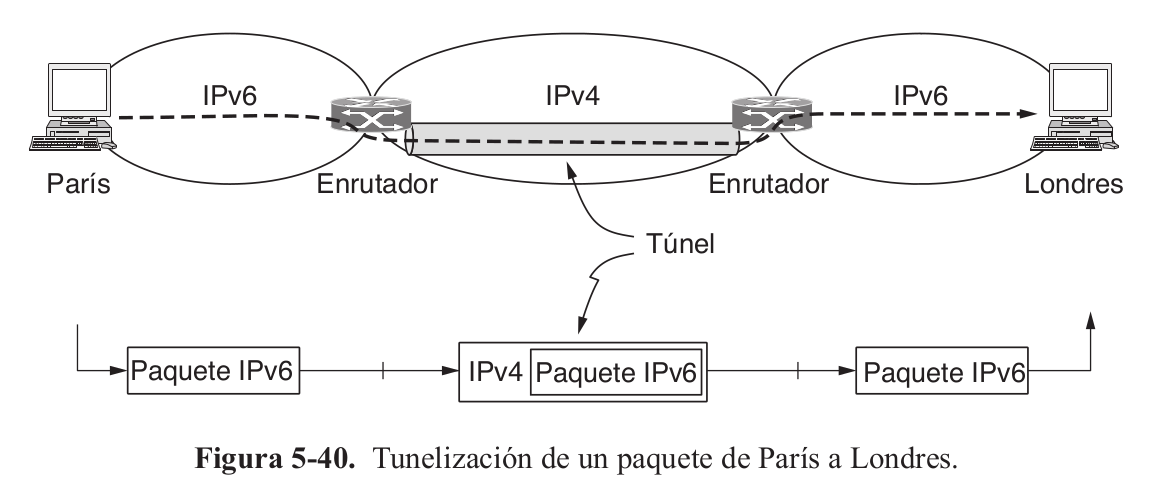
\includegraphics[scale=0.3]{./imagenes/entunelamiento.png}
	\end{center}

	\subsection{Fragmentación}
	Cuando un paquete grande quiere viajar a través de una red cuyo tamaño máximo de paquete es demasiado pequeño nos encontramos con que debemos \textbf{fragmentar el paquete}.
	Existen dos estrategias:

	\begin{itemize}
		\item \textbf{Transparente:} En este método, cuando un paquete de tamaño excesivo
llega a un enrutador, este lo divide en fragmentos. Cada fragmento es dirigido al mismo enrutador
de salida, en donde se recombinan las piezas. De esta manera se ha hecho transparente el paso a
través de la red de paquete pequeño. Las redes subsecuentes ni siquiera se enteran de que ha ocurrido
una fragmentación.
		\item \textbf{No transparente:} Una vez que se ha fragmentado un paquete, cada fragmento se trata como si fuera un paquete
original. Los enrutadores pasan los fragmentos y la recombinación
ocurre sólo en el host de destino.
	\end{itemize}

	\begin{center}
		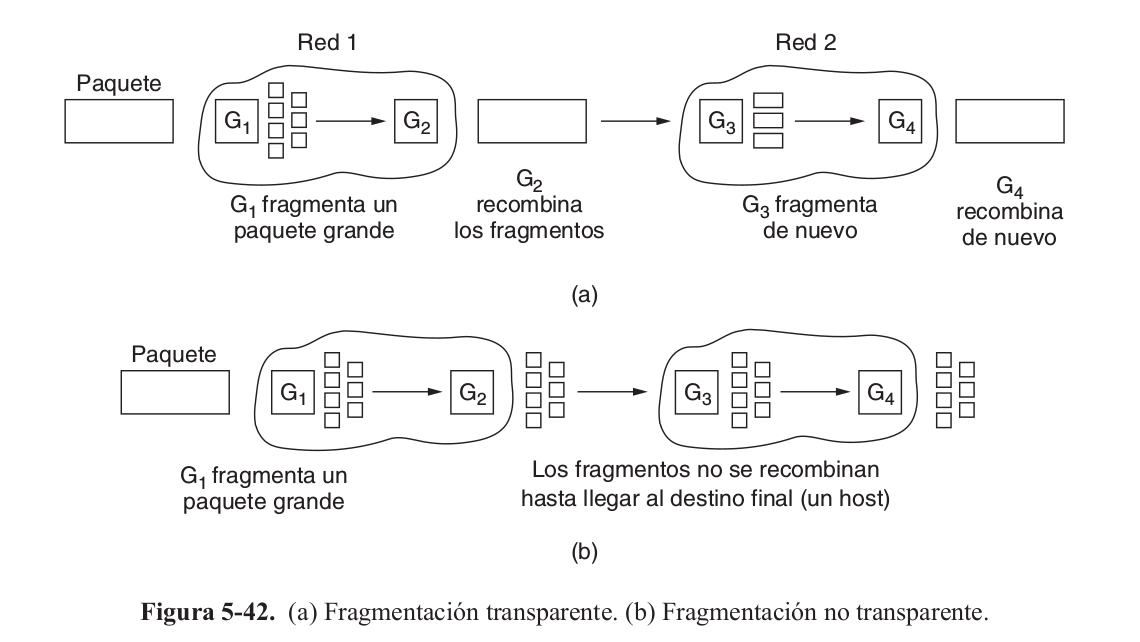
\includegraphics[scale=0.3]{./imagenes/fragmentacion.png}
	\end{center}

\section{La capa de internet}

	\subsection{Principios de la capa de red}
	\begin{itemize}
		\item 1. Asegurarse de que funciona. No termine el diseño o estándar hasta que múltiples prototipos se hayan comunicado entre sí de manera exitosa.
 		\item 2. Mantener la simplicidad. Cuando tenga duda, utilice la solución más simple.
 		\item 3. Elegir opciones claras. Si hay varias maneras para realizar la misma tarea, elija sólo una.
  		\item 4. Explotar la modularidad. Este principio lleva directamente a la idea de tener pilas de protocolos, cuyas capas sean independientes entre sí.
		\item 5. Prevenir la heterogeneidad. En cualquier red grande habrán diferentes tipos de hardware, facilidades de transmisión y aplicaciones. Para manejarlos, el diseño de la red debe ser simple, general y flexible.
		\item 6. Evitar las opciones y parámetros estáticos. Si los parámetros son inevitables (por ejemplo, el tamaño máximo del paquete), es mejor hacer que el emisor y el receptor negocien un valor que definir opciones fijas.
		\item 7. Buscar un buen diseño no es necesario que sea perfecto. Con frecuencia, los diseñadores tienen
un buen diseño pero éste no puede manejar algún caso especial.
		\item 8. Ser estricto cuando envíe y tolerante cuando reciba. En otras palabras, sólo envíe paquetes que
cumplan rigurosamente con los estándares, pero espere paquetes que tal vez no cumplan del todo
y trate de lidiar con ellos.
		\item 9. Pensar en la escalabilidad. Si el sistema debe manejar de manera efectiva millones de hosts y
miles de millones de usuarios, la carga se debe dispersar de la manera más equitativa posible entre los recursos disponibles.
		\item 10. Considerar el desempeño y el costo. Si una red tiene un desempeño pobre o un costo exagerado,
nadie la utilizará.
	\end{itemize}

	\subsection{El protocolo IP versión 4}
	Un datagrama IPv4 consiste en dos partes: el encabezado y el cuerpo o carga útil. El encabezado tiene una parte fija de 20 bytes y una parte opcional de longitud variable. Los bits se transmiten en orden de izquierda a derecha y de arriba hacia abajo, comenzando por el bit de mayor orden del campo \textit{Versión}.
	
	\begin{center}
		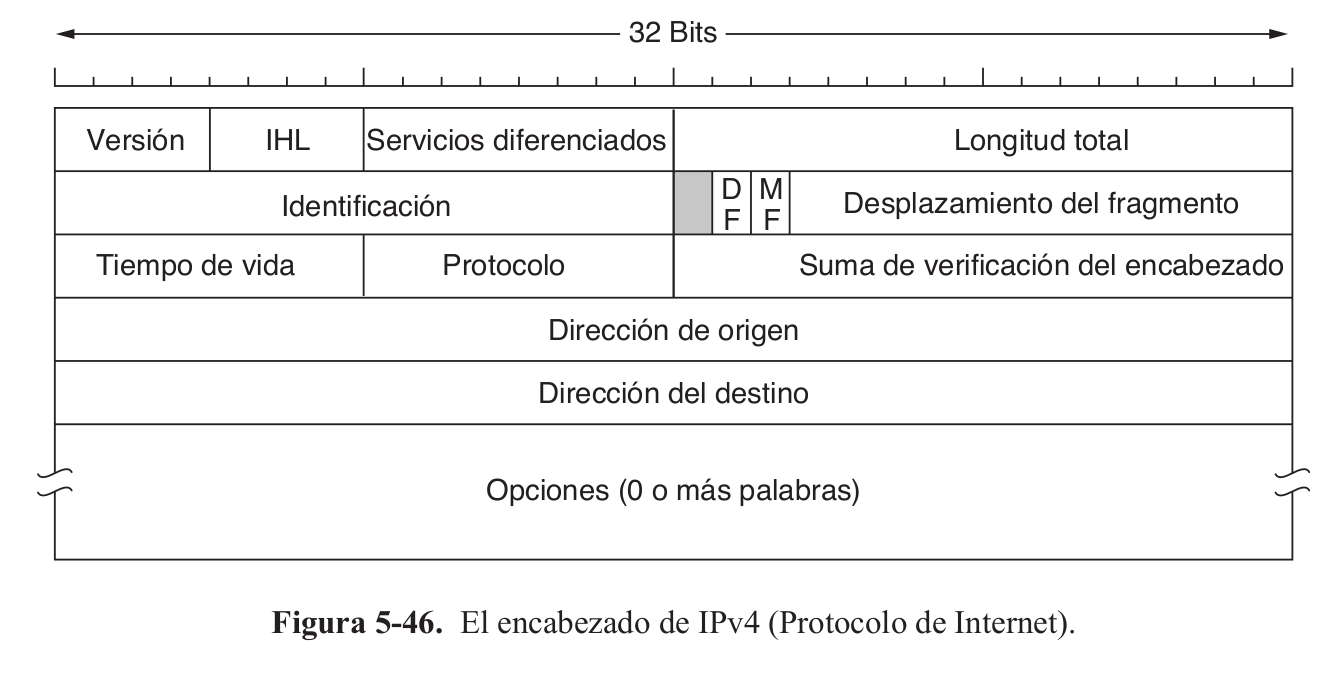
\includegraphics[scale=0.3]{./imagenes/encabezadoIP.png} 
	\end{center}
	
	\begin{itemize}
		\item \textbf{Versión:} (\textit{4 bits}) Lleva el registro de la versión del protocolo a la que pertenece el datagrama (p.ej. IPv4).
		\item \textbf{IHL:} (\textit{4 bits}) Indica la cantidad de palabras de 32 bits en el encabezado. El valor mínimo es de 5 (se usa cuando no hay opciones); el valor
máximo es de 15, lo que limita el encabezado a 60 bytes, y por lo tanto el campo de opciones es de 40 bytes.
		\item \textbf{Servicios Diferenciados:} (\textit{8 bits}) Este es uno de los pocos campos que ha cambiado su significado, originalmente era \textit{Tipo de Servicio}. Contaba con 6 bits, de los cuales , 3 eran para indicar la prioridad y 3 para indicar si a un host le
preocupaba más el \textit{delay}, \textit{throughput} o la \textit{reliability}. Y los ultimos 2 bits no se utilizaban.
		\item \textbf{Longitud Total:} (\textit{16 bits}) Incluye todo el datagrama, tanto el encabezado como los datos. La longitud máxima es de 65535 bytes.
		\item \textbf{Identificación:} (\textit{16 bits}) Es necesario para que el host de destino determine a qué datagrama pertenece un
fragmento recién llegado. (Todos los fragmentos de un datagrama contienen el mismo valor de identificación)
		\item A continuación viene un bit sin uso
		\item \textbf{DF:} (\textit{1 bit}) Cuando esta fijado en 1 significa no fragmentar.
		\item \textbf{MF:} (\textit{1 bit}) Significa mas fragmentos, todos los fragmentos excepto el último tienen este bit activado.
		\item \textbf{Desplazamiento del fragmento:} (13 bits) Indica a qué parte del paquete actual pertenece este fragmento. Todos los fragmentos excepto el último del datagrama deben ser un múltiplo de 8 bytes, que es la unidad de fragmentos elemental. Dado que se proporcionan 13 bits, puede haber un máximo de 8 192 fragmentos.
		\item \textbf{Tiempo de vida:} (\textit{8 bits}) Es un contador que se utiliza para limitar el tiempo de vida de un paquete.
		\item \textbf{Protocolo:} (\textit{8 bits}) Le indica a cuál proceso de transporte debe entregar el paquete.
		\item \textbf{Suma de verificación:} (\textit{16bits}) El algoritmo suma todas las medias palabras de 16 bits del encabezado a medida que vayan llegando, mediante el uso de la aritmética de complemento a uno, y después obtiene el complemento a uno del resultado.
		\item \textbf{Dirección de Origen y Destino:} (\textit{32 bits c/u}) Indican la dirección IP de las interfaces de red de la fuente y del destino.
		\item \textbf{Opciones:} El campo de opciones ha sido diseñado para proveer un escape para permitir versiones subsecuentes del protocolo que incluyan
información no presente en el diseño original, para permitir a los experimentadores probar nuevas ideas y evitar alojar bits de encabezado a información que es raramente necesitada. Las opciones son de longitud variable., y cada opción comienza con un código de 1 byte para identificarla. Algunas opciones tienen un campo de longitud de opción y luego uno o más bytes de datos. El campo de opciones ocupa un múltiplo de 4 bytes.
	\end{itemize}
	
	\begin{center}
		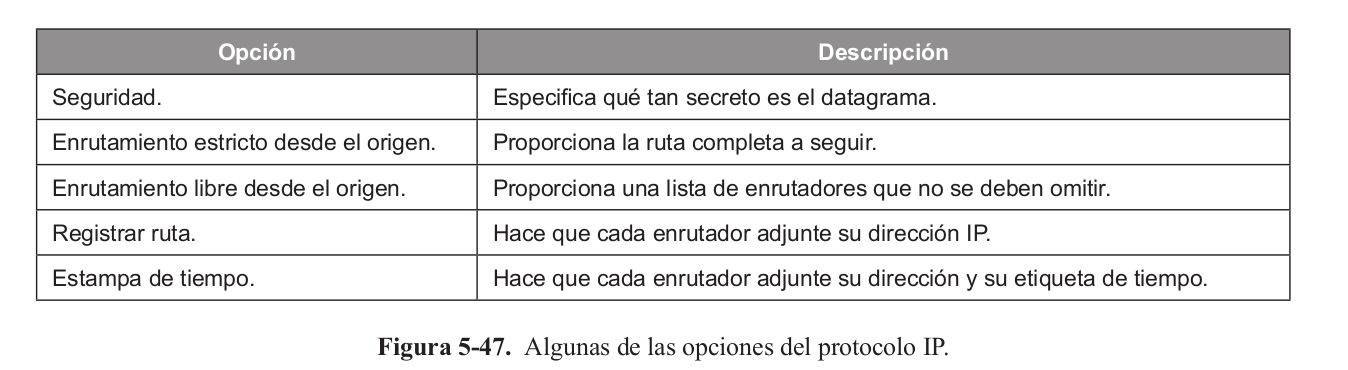
\includegraphics[scale=0.3]{./imagenes/opcionesIP.png} 
	\end{center}
	\subsection{Direcciónes IP}
	Una característica que define a IPv4 consiste en sus direcciones de 32 bits. Cada host y enrutador de Internet tiene una dirección IP que se puede usar en los campos Dirección de origen y Dirección de destino de los paquetes IP. Es importante tener en cuenta que una dirección IP en realidad no se refiere a un host, sino
a una interfaz de red, por lo que si un host está en dos redes, debe tener dos direcciones IP.
	\subsubsection{Prefijos}
	A diferencia de las direcciones Ethernet, las direcciones IP son jerárquicas. Cada dirección de 32 bits está
	compuesta de una porción de red de longitud variable en los bits superiores, y de una porción de host en
	los bits inferiores. La porción de red tiene el mismo valor para todos los hosts en una sola red, como una
	LAN Ethernet. Esto significa que una red corresponde a un bloque contiguo de espacio de direcciones IP.
	A este bloque se le llama prefijo.
	\par En nuestro ejemplo, si el prefijo contiene $ 2^{8}$ direccciones y, por lo
	tanto, deja 24 bits para la porción de red, se escribe como 128.208.0.0/24.
	\par Como la longitud del prefijo no se puede inferir sólo a partir de la dirección IP, los protocolos de enrutamiento deben transportar los prefijos hasta los enrutadores. Algunas veces los prefijos se
describen simplemente mediante su longitud, como en un “/16”, Cuando se escribe
de esta forma, se denomina máscara de subred. Se puede aplicar un AND a la máscara de subred
con la dirección IP para extraer sólo la porción de la red.

	\begin{center}
		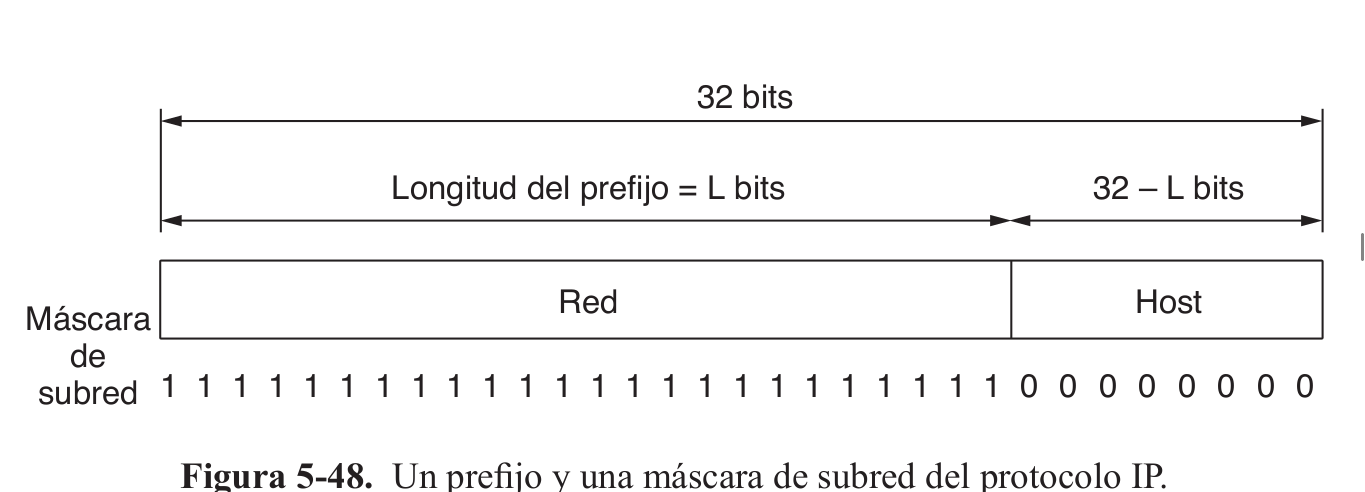
\includegraphics[scale=0.3]{./imagenes/prefijomascara.png} 
	\end{center}

	\subsubsection{Subredes}
	
	La idea es permitir a una red que sea dividida en varias partes para uso interno pero que todavía actúe como una red simple para el mundo externo.
	Cada subred puede ser una LAN que tiene un enrutador. Fuera de la red, una subred no es visible.	
	\par Cuando llega un paquete, el enrutador analiza su dirección de destino y verifica a qué subred pertenece. Para ello, el enrutador aplica un AND a la dirección del destino con la máscara para cada subred y verifica que el resultado sea el prefijo correspondiente.
	
	\subsection{CIDR}

	El objetivo de CIDR es reducir los tamaños de las tablas de enrutamiento. Para ello, se aplica la misma perspectiva que en las subredes: los enrutadores en distintas 			ubicaciones pueden saber acerca de una dirección IP dada que pertenece a prefijos de distintas zonas. A este proceso se le conoce como \textbf{agregación de prefijos}. 		\par Algunas veces al prefijo más grande resultante se le denomina superred para contrastar con las subredes como la división de bloques
de direcciones.
	\par Cuando llega un paquete primero se extrae su dirección de destino IP, luego se analiza la tabla de enrutamiento entrada por entrada. Hacer AND de la máscara de la entrada con la dirección de destino y comparar el resultado con la dirección IP de inicio de la subred de la entrada. Es posible que coincidan entradas múltiples (con diferentes longitudes de máscara de subred), en cuyo caso se usa la máscara más larga.
	
	\begin{center}
		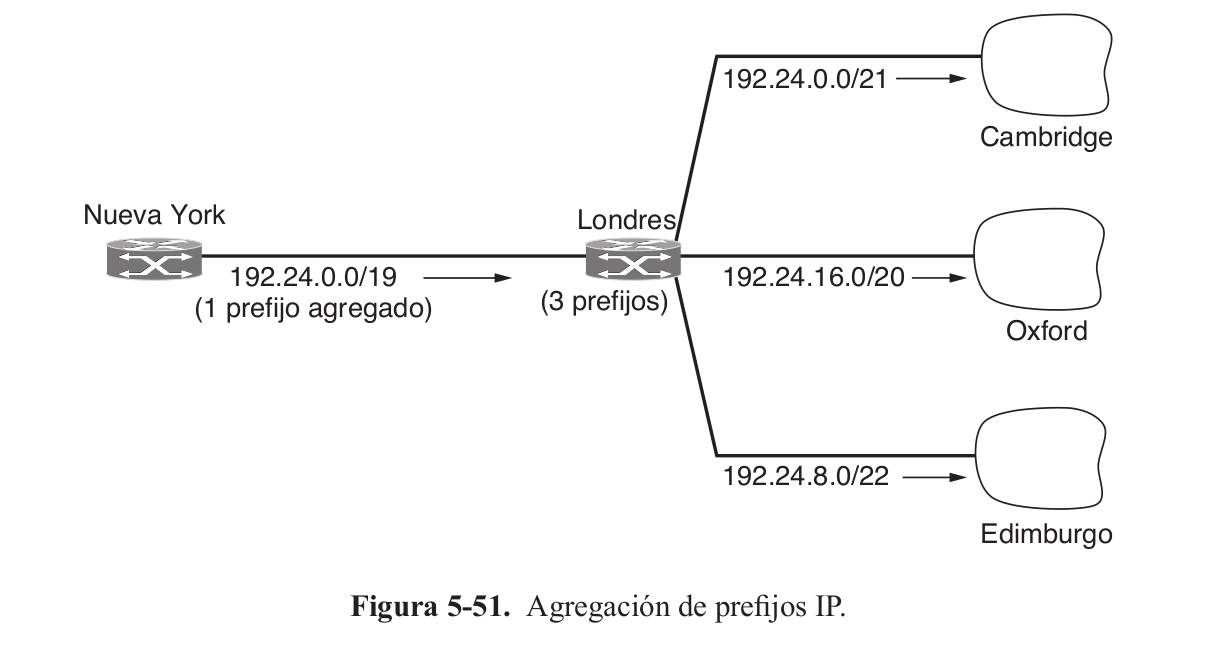
\includegraphics[scale=0.3]{./imagenes/agregacionPrefijosIP.png} 
	\end{center}	
	
	\subsubsection{Direccionamiento con clases}
	Antes de 1993, las direcciones IP se dividían en las cinco categorías. Esta asignación se denominó direccionamiento con clases.	
	
	\begin{center}
		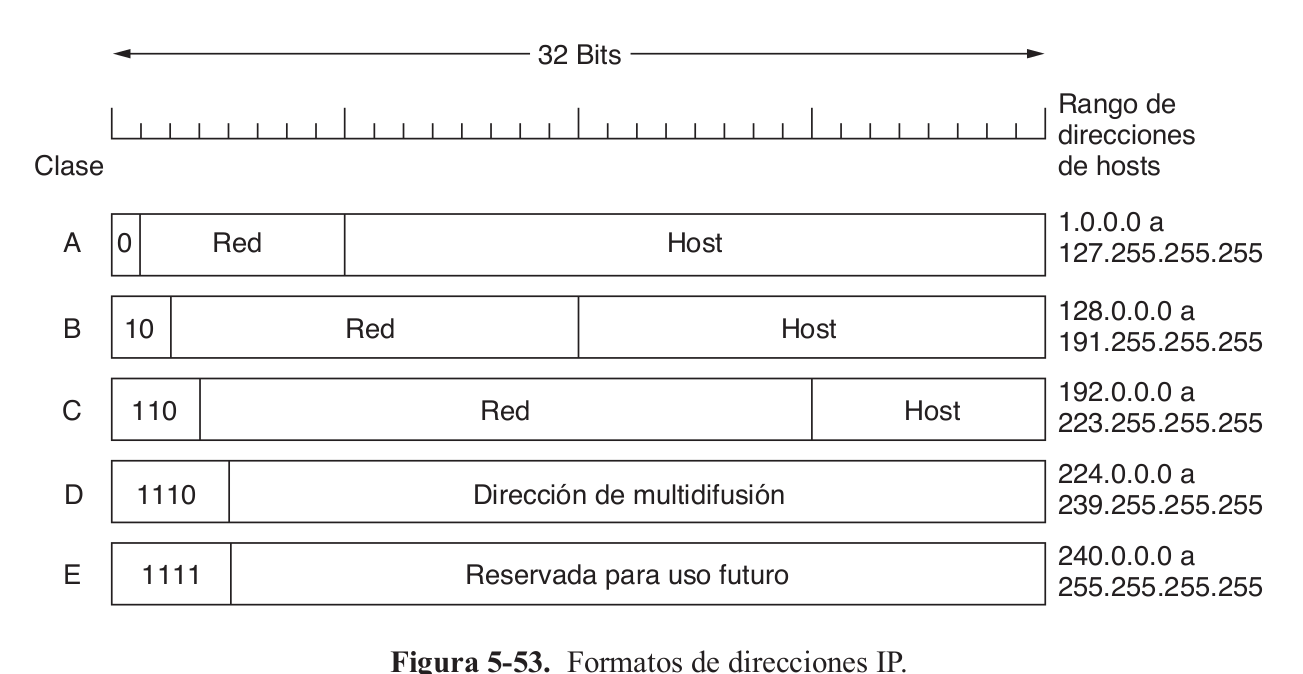
\includegraphics[scale=0.3]{./imagenes/clasesIP.png} 
	\end{center}	
	La dirección IP 0.0.0.0, que es la dirección más baja, es utilizada por los hosts al momento de encen-
derlos. Significa “esta red” o “este host”. Las direcciones IP con 0 como número de red se refieren a la
red actual.
	\par La dirección que
consiste sólo en 1s, o 255.255.255.255 (la dirección más alta), se utiliza para indicar a todos los hosts
en la red especificada. Permite la difusión en la red local, por lo general una LAN.
	\par Por último, todas
las direcciones de la forma 127.xx.yy.zz se reservan para las pruebas de loopback. Los paquetes que se
envían a esa dirección no se ponen en el cable; se procesan en forma local y se tratan como si fueran
paquetes entrantes.
	\subsection{NAT}
	
	La idea básica detrás de NAT es que el ISP asigne a cada hogar o negocio una sola dirección IP
(o a lo más, una pequeña cantidad de éstas) para el tráfico de Internet. Dentro de la red del cliente, cada
computadora obtiene una dirección IP única, la cual se utiliza para enrutar el tráfico interno. Sin embargo, justo antes de que un paquete salga de la red del cliente y vaya al ISP, la dirección IP única interna se traduce a la dirección IP pública compartida. Esta traducción hace uso de los tres rangos de direcciones
IP que se han declarado como privados. Las redes pueden utilizarlos de manera interna como deseen. La
única regla es que no pueden aparecer paquetes que contengan estas mismas direcciones en Internet. Los
tres rangos reservados son:
\par
\par
	\begin{center}
	

	\begin{tabular}{ccc}
	10.0.0.0 & -10.255.255.255 & (16,777,216 hosts) \\ 
	\par
	172.16.0.0 & 172.31.255.255 & (1,048,576 hosts) \\ 
	\par
	192.168.0.0 & 192.168.255.255 & (65,536 hosts) \\ 
	\par
	\end{tabular} 
	\end{center}
	\par
	\par En la figura 5-55 se muestra la operación de NAT. Dentro de las premisas del cliente, cada máquina
tiene una dirección única de la forma 10.x.y.z. Sin embargo, antes de que un paquete salga de las premisas
del cliente, pasa a través de una caja NAT que convierte la dirección IP de origen interna, 10.0.0.1 en
la figura, a la dirección IP verdadera del cliente, 198.60.42.12 en este ejemplo.

\par Cuando un proceso desea establecer una conexión TCP con un proceso remoto, se conecta a un puerto
TCP sin usar en su propia máquina. Éste se conoce como \textbf{puerto de origen} y le indica al código TCP dónde enviar los paquetes entrantes que pertenecen a esta conexión. El proceso también proporciona un \textbf{puerto de destino} para indicar a quién se deben dar los paquetes en el lado remoto. Los puertos 0-1023 se reservan para los servicios conocidos.

\par Siempre que un paquete de salida entra en la caja NAT, la dirección de origen 10.x.y.z se reemplaza por la verdadera dirección IP del cliente. Además, el campo Puerto de origen TCP se reemplaza por un índice en la tabla de traducción de 65 536 entradas de la caja NAT. Esta entrada de la tabla contiene el puerto de
origen y la dirección IP originales. Finalmente, las sumas de verificación de los encabezados IP y TCP se recalculan e insertan en el paquete. Es necesario reemplazar el Puerto de origen, porque podría ocurrir que ambas conexiones de las máquinas 10.0.0.1 y 10.0.0.2 usaran el puerto 5 000, por ejemplo, así que el
Puerto de origen no basta por sí solo para identificar el proceso de envío. Cuando un paquete llega a la caja NAT desde el ISP, el Puerto de origen en el encabezado TCP se
extrae y utiliza como un índice en la tabla de asignación de la caja NAT. Desde la entrada localizada, la dirección IP interna y el Puerto de origen TCP se extraen e insertan en el paquete. Luego, las sumas de verificación de IP y TCP se recalculan e insertan en el paquete. Entonces el paquete se pasa al enrutador
del cliente para su entrega normal mediante el uso de la dirección 10.x.y.z.

\subsection{Protocolos de control de Internet}

\subsubsection{ARP: Protocolo de Resolución de Direcciones}

	\par Aunque en internet una máquina tiene una o más direcciones IP, estas no pueden usarse para enviar paquetes debido a que el hardware de la capa de enlace de datos no entiende las direcciones de internet. Hoy día la mayoría de los hosts de las compañías y las universidades se une a una LAN por una tarjeta de red que solo entiende direcciones LAN. Por ejemplo cada tarjeta Ethernet viene provista de fábrica con una dirección Ethernet de 48 bits, las tarjetas envían y reciben tramas basadas en direcciones Ethernet de 48 bits pero no saben nada de direcciones IP.
	
	\par La pregunta ahora es: ¿Cómo se convierten las direcciones IP en direcciones de la capa de enlace de datos, como Ethernet?. La idea sería que el host de origen dé salida a un paquete de difusión hacia Ethernet preguntando: ¿Quién posee una dirección IP w.x.y.z ?. La difusión llegará a cada máquina en Ethernet y cada una verificará su dirección IP. Al host de destino le bastará con responder con su dirección de Ethernet E y de este modo el host de origen aprende que la dirección IP de w.x.y.z está en el host con la dirección de Ethernet E. Casi cada máquina en Internet ejecuta ARP.

	\par La ventaja de usar ARP es la sencillez. Solo se tiene que asignar a cada máquina una dirección IP y decidir respecto de las máscaras de subred. ARP hace el resto.
	
	\par Se pueden hacer optimizaciones para que ARP funcione con más eficiencia.
	
		\begin{itemize}
			\item \underline{Optimización 1:} una vez que una máquina ha ejecutado ARP, guarda el resultado en caso de que en poco tiempo tenga que ponerse de nuevo en contacto con la misma máquina. La próxima vez encontrará la correspondencia en su propia caché, eliminando así la necesidad de una segunda difusión.

			\item \underline{Optimización 2:} en muchos casos el host de destino necesitará devolver una respuesta, forzando también a que se ejecute el ARP para determinar la dirección Ethernet del emisor. Esta difusión de ARP puede evitarse teniendo el host de origen que incluir su correspondencia IP a Ethernet en el paquete ARP. Cuando la difusión de ARP llega al host de destino, se introduce la dirección IP y de Ethernet del origen en el caché del host 2 para su uso futuro.
			
			\item \underline{Optimización 3:} cada máquina difunde su correspondencia cuando arranca, esto se hace mediante un ARP que busca su propia dirección IP. No debe haber una respuesta, pero un efecto lateral de la difusión es hacer una entrada en el caché ARP de todas las máquinas, si llega inesperadamente una respuesta, es que la misma dirección IP se ha asignado a dos máquinas. La más reciente debe avisar y no arrancar.
		\end{itemize}

	\par Para permitir que las asociaciones cambien, por ejemplo, al configurar un host para que use una nueva dirección IP (pero que mantenga su vieja dirección Ethernet), las entradas en la caché ARP deben expirar después de unos cuantos minutos.
	
	\par Cuando el host de origen y el host de destino están en distintas Ethernet LAN 1 y LAN 2 respectivamente separadas por enrutadores, si se usa ARP fallará ya que el host de destino no verá la difusión (los enrutadores no envían difusiones a nivel Ethernet). Veamos este problema con un ejemplo en la siguiente figura.
	
		\begin{center}
			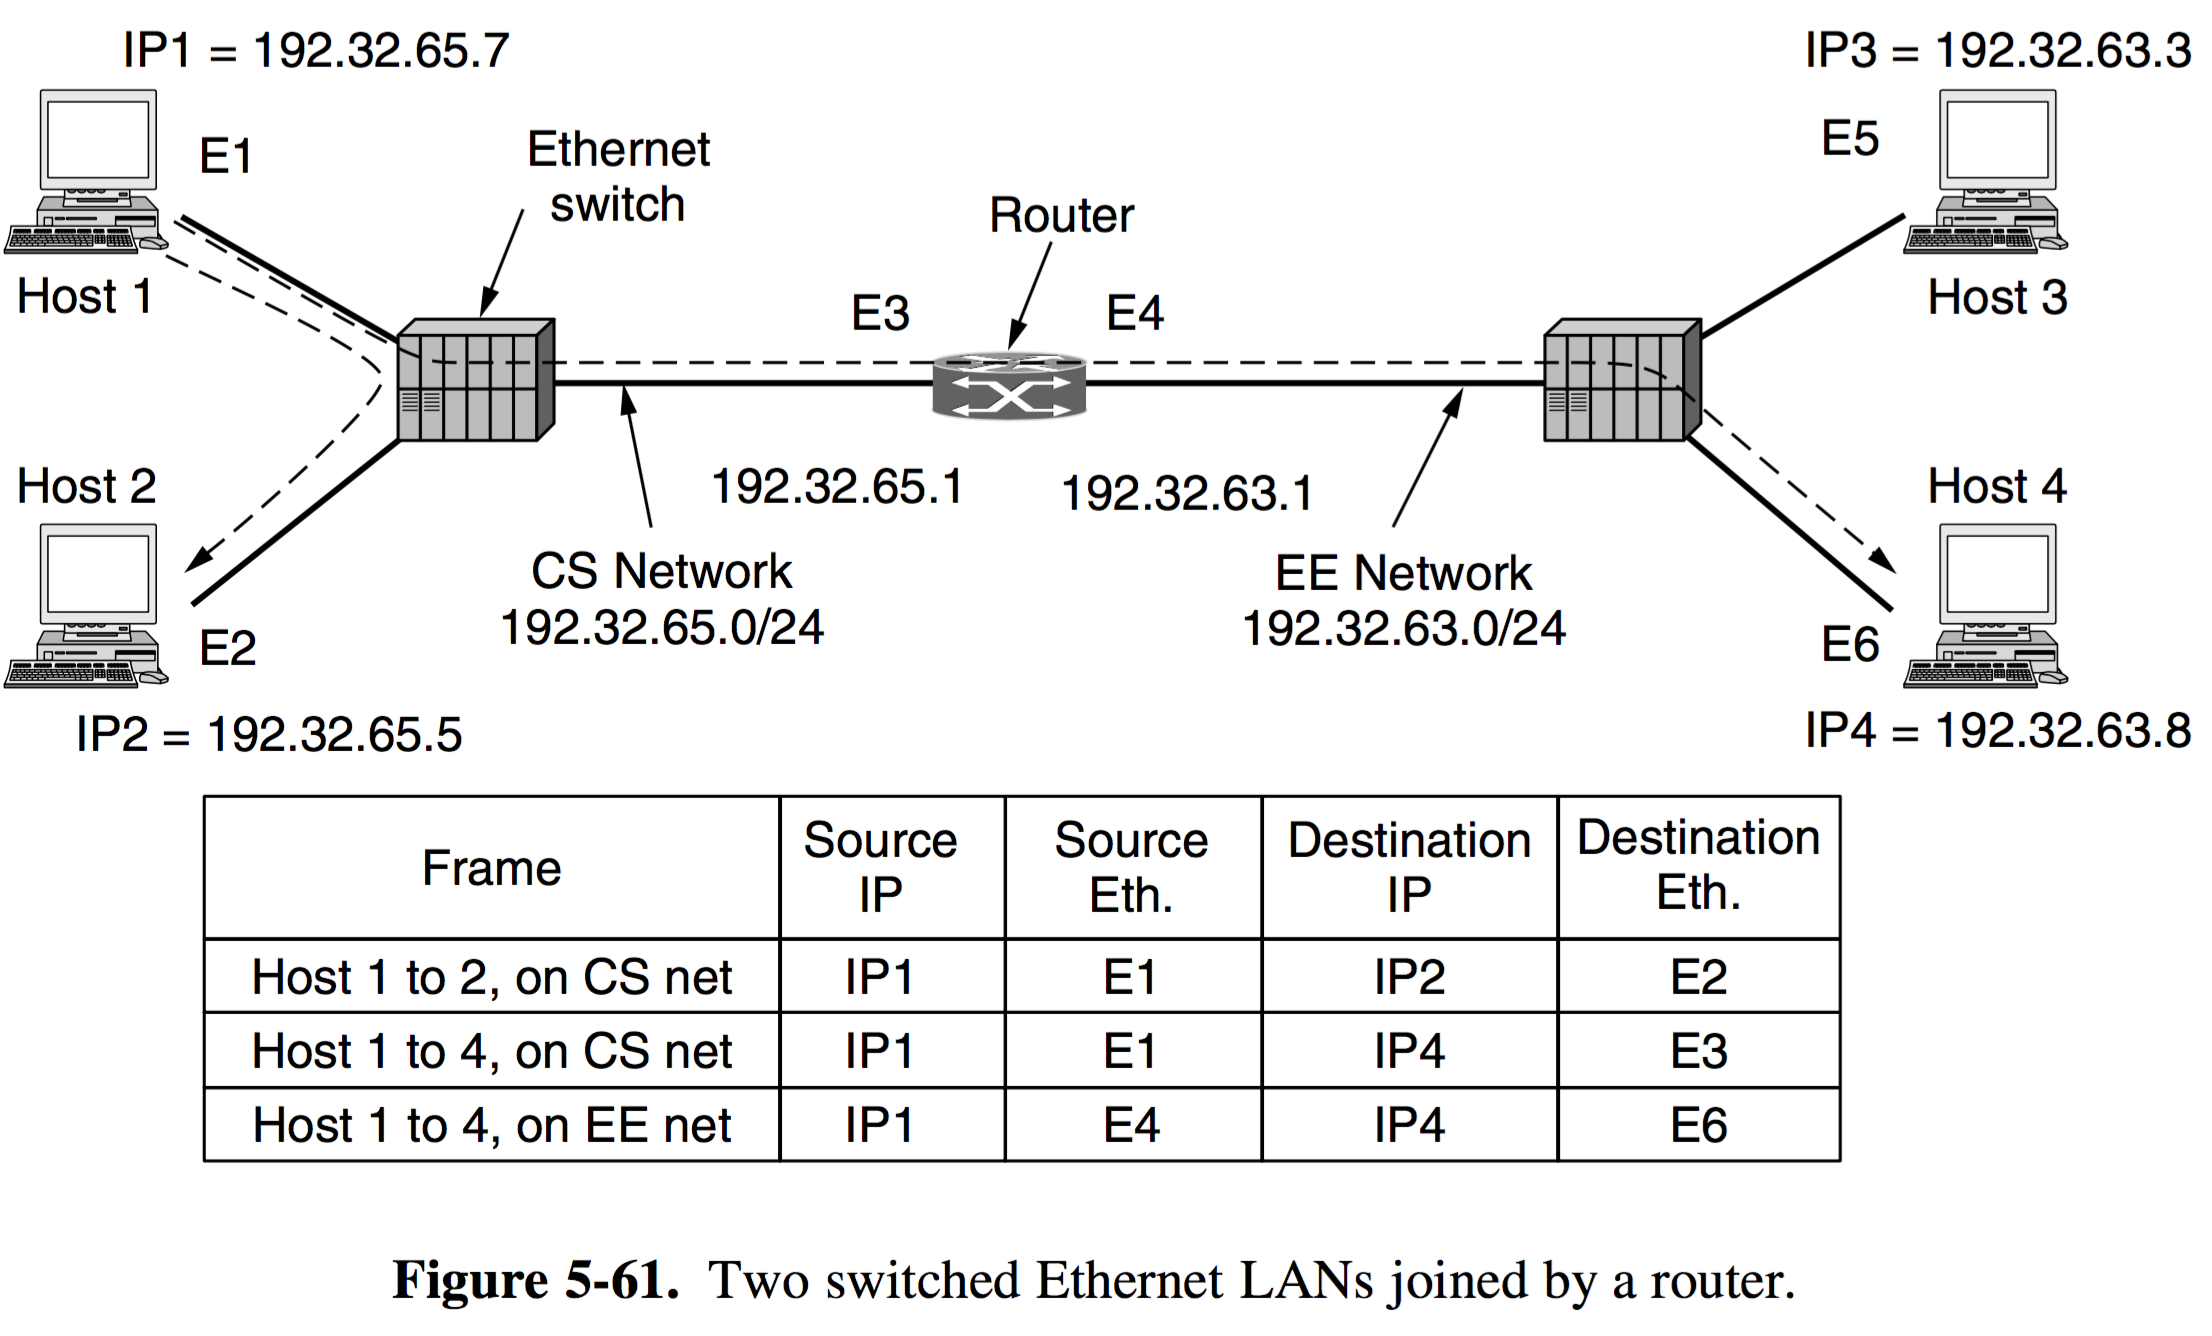
\includegraphics[width=9cm, height=6cm]{./imagenes/arp.png} 
		\end{center}

	\par Viendo la figura de arriba, supongamos que el \textit{host 1} quiere enviar un paquete al \textit{host 4} (192.32.63.8) en la red IE. El \textit{host 1} verá que la dirección IP de destino no está en la red CS. Sabe enviar todo ese tráfico fuera de la red al enrutador, el cual también se conoce como puerta de enlace predeterminada. Por convención, la puerta de enlace predeterminada es la dirección más baja en la red (198.31.65.1). Para enviar una trama al enrutador, el \textit{host 1} debe conocer de todas formas la dirección Ethernet de la interfaz del enrutador en la red CS. Para descubrirla envía una difusión ARP para 198.31.65.1, a partir de la cual aprende E3. Después envía la trama. Los mismos mecanismos de búsqueda se utilizan para enviar un paquete de un enrutador al siguiente, a través de una secuencia de enrutadores en una ruta de Internet.
	
	\par Cuando la placa de red de Ethernet del enrutador recibe esta trama, entrega el paquete al software IP. Sabe con base en las máscaras de red que el paquete se debe enviar a la red IE, en donde alcanzará al \textit{host 4}. Si el enrutador no conoce la dirección Ethernet para el \textit{host 4}, entonces usará ARP de nuevo. Las direcciones Ethernet cambian con la trama en cada red, mientras que las direcciones IP permanecen constantes (puesto que indican las terminales a través de todas las redes interconectadas).
	
\subsection{OSPF: un protocolo de enrutamiento de puerta de enlace interior}
	\par Internet se compone de una gran cantidad de \textbf{Sistemas Autónomos}. Cada uno de ellos es manejado por una organización diferente y puede usar su propio algoritmo interno de enrutamiento. Un algoritmo de enrutamiento dentro de un sistema autónomo se llama \textbf{protocolo de puerta de enlace interior (IGP)}; un algoritmo para enrutamiento entre sistemas autónomos se llama protocolo de \textbf{puerta de enlace exterior (EGP)}.

	\par El protocolo de puerta de enlace interior original en internet era un protocolo de vector de distancia (\textit{RIP}). Fue reemplazado en 1979 por un protocolo de estado de enlace. Luego en 1988 se definió un sucesor llamado OSPF (\textbf{Open Shorted Path First}), que se volvió una norma en 1990. Ahora la mayoría de vendedores de enrutadores lo apoyan.
	
	\par OSPF tenía una larga lista de requerimientos por cumplir. El algoritmo se tenía que apoyar en una variedad de métricas de distancia como distancia física, retardo, etc. Tenía que ser un algoritmo dinámico que se adaptara rápida y automáticamente a los cambios en la topología. Debía apoyar el enrutamiento con base en el tipo de servicio. El nuevo protocolo tenía que dirigir el tráfico en tiempo real de una manera y el resto del tráfico de otra.
	
	\par El nuevo protocolo tenía que balancear la carga, dividiéndola en líneas múltiples. La mayoría de los protocolos anteriores enviaba todos los paquetes por la mejor ruta, incluso si había dos rutas buenas.

	\par Se necesitaba apoyo para los sistemas jerárquicos. Había que tratar con enrutadores que se conectan a internet por medio de un túnel.

	\par OSPF soporta tres tipos de conexiones y redes:

		\begin{enumerate}
			\item Las líneas punto a punto exactamente entre dos enrutadores.
			\item Redes de multiacceso con difusión (la mayoría de las LAN).
			\item Redes de multiacceso con muchos enrutadores, cada uno de los cuales se puede comunicar directamente con los otros.
		\end{enumerate}

	\par La siguiente figura muestra un sistema autónomo con los tres tipos de redes. En ella se omiten los hosts, ya que en general no desempeñan ningún papel en OSPF.

		\begin{center}
			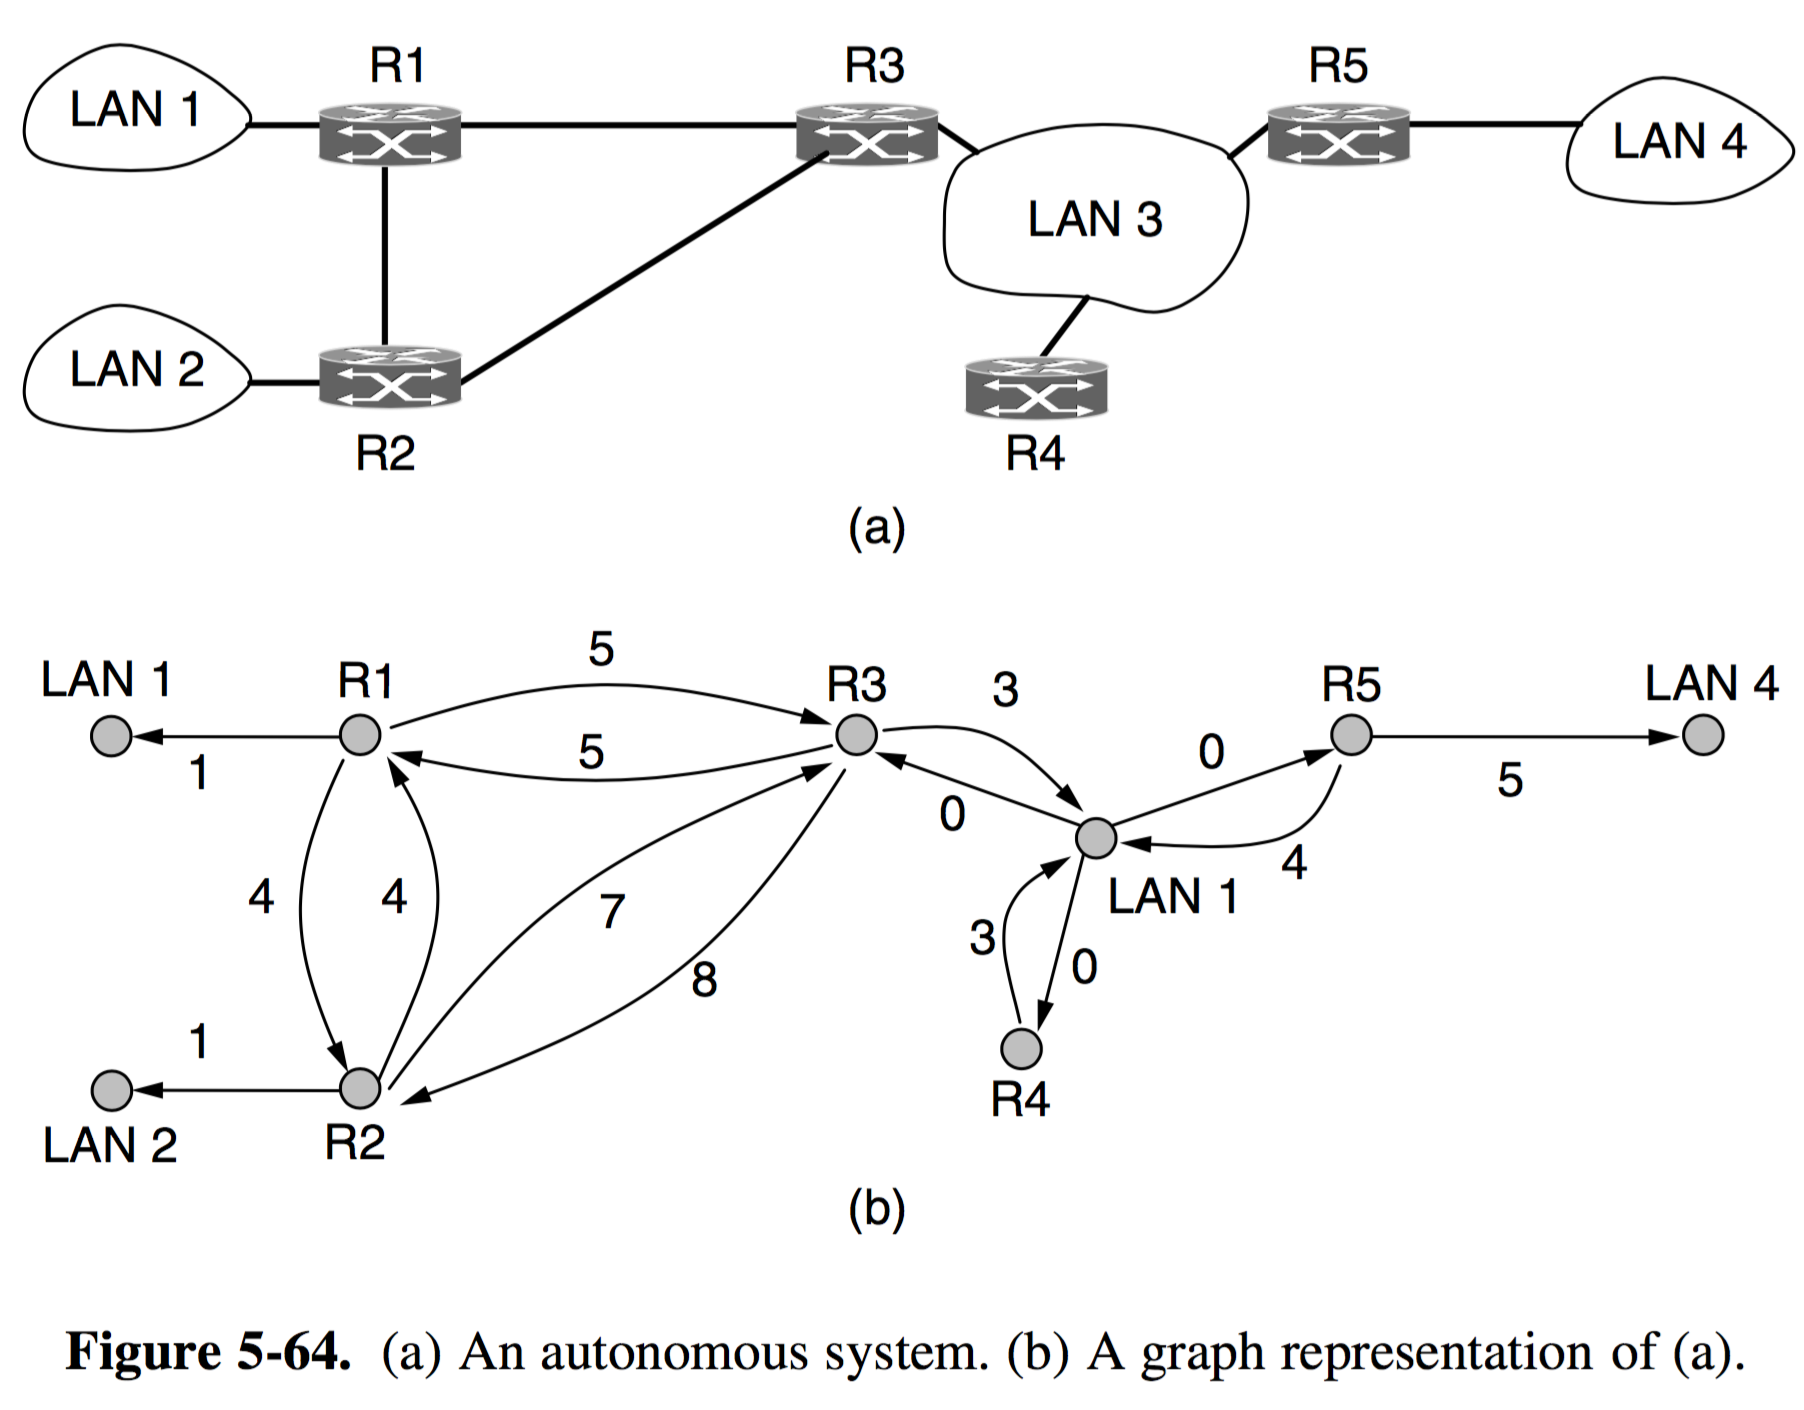
\includegraphics[width=8cm, height=5cm]{./imagenes/ospf.png} 
		\end{center}

	\par OSPF abstrae la topología en un \textbf{grafo dirigido} en el que a cada arco se asigna un costo (distancia, retardo, etc.). Una conexión \textit{punto-punto} entre dos enrutadores se representa por un par de arcos, uno en cada dirección, donde sus pesos pueden ser diferentes. Una red de multiacceso de difusión se representa con un nodo
para la red en sí, más un nodo para cada enrutador. Los arcos desde el nodo de la red a los enrutadores tienen peso 0, sin embargo son importantes puesto que sin ellos no habrá una ruta a través de la red.

	\par Luego de la construcción del grafo se utiliza al algoritmo de \textit{Dijkstra} para hacer que cada enrutador calcule la ruta más corta desde sí mismo hacia todos los demás nodos. Se pueden encontrar varias rutas que sean igual de cortas. En este caso, OSPF recuerda el conjunto de rutas más cortas y, durante el envío de paquetes, el tráfico se divide entre ellas. Este proceso ayuda a balancear la carga y se conoce como ECMP (\textbf{Equal Cost MultiPath}).

	\par Muchos de los sistemas autónomos (AS) en Internet son grandes por sí mismos y nada sencillos de administrar. Para trabajar a esta escala, OSPF permite dividir un AS en áreas numeradas, en donde un área es una red o un conjunto de redes contiguas y cada área puede contener varias redes dentro de sí misma. Las áreas no se traslapan, algunos enrutadores no necesitan pertenecer a ningún área. Los enrutadores que están totalmente dentro de un área se llaman \textbf{enrutadores internos}.

	\par Cada Sistema Autónomo tiene un área de \textbf{red dorsal}, llamada área 0. Los enrutadores en esta área se llaman \textbf{enrutadores dorsales}. Todas las áreas se conectan a la red dorsal, posiblemente mediante túneles, de modo que es posible ir desde cualquier área en el AS a cualquier otra área en el AS mediante la red dorsal. En el grafo, un túnel se representa como otro arco más con un costo. Al igual que con otras áreas, la topología de la red troncal no es visible fuera de esta.

	\par Cada enrutador que se conecta a dos o más áreas se llama \textbf{enrutador de borde de área} (\textit{EBA}) y es parte de la red dorsal y a la vez de una o más áreas.

	\par El \textbf{enrutador de borde de sistema autónomo} (\textit{EBSA}) inyecta en el área rutas a destinos externos en otros AS. Las rutas externas aparecen como destinos que pueden ser alcanzados vía un EBSA con algún costo. Una ruta externa puede ser inyectada a uno o más EBSA.

	\begin{center}
			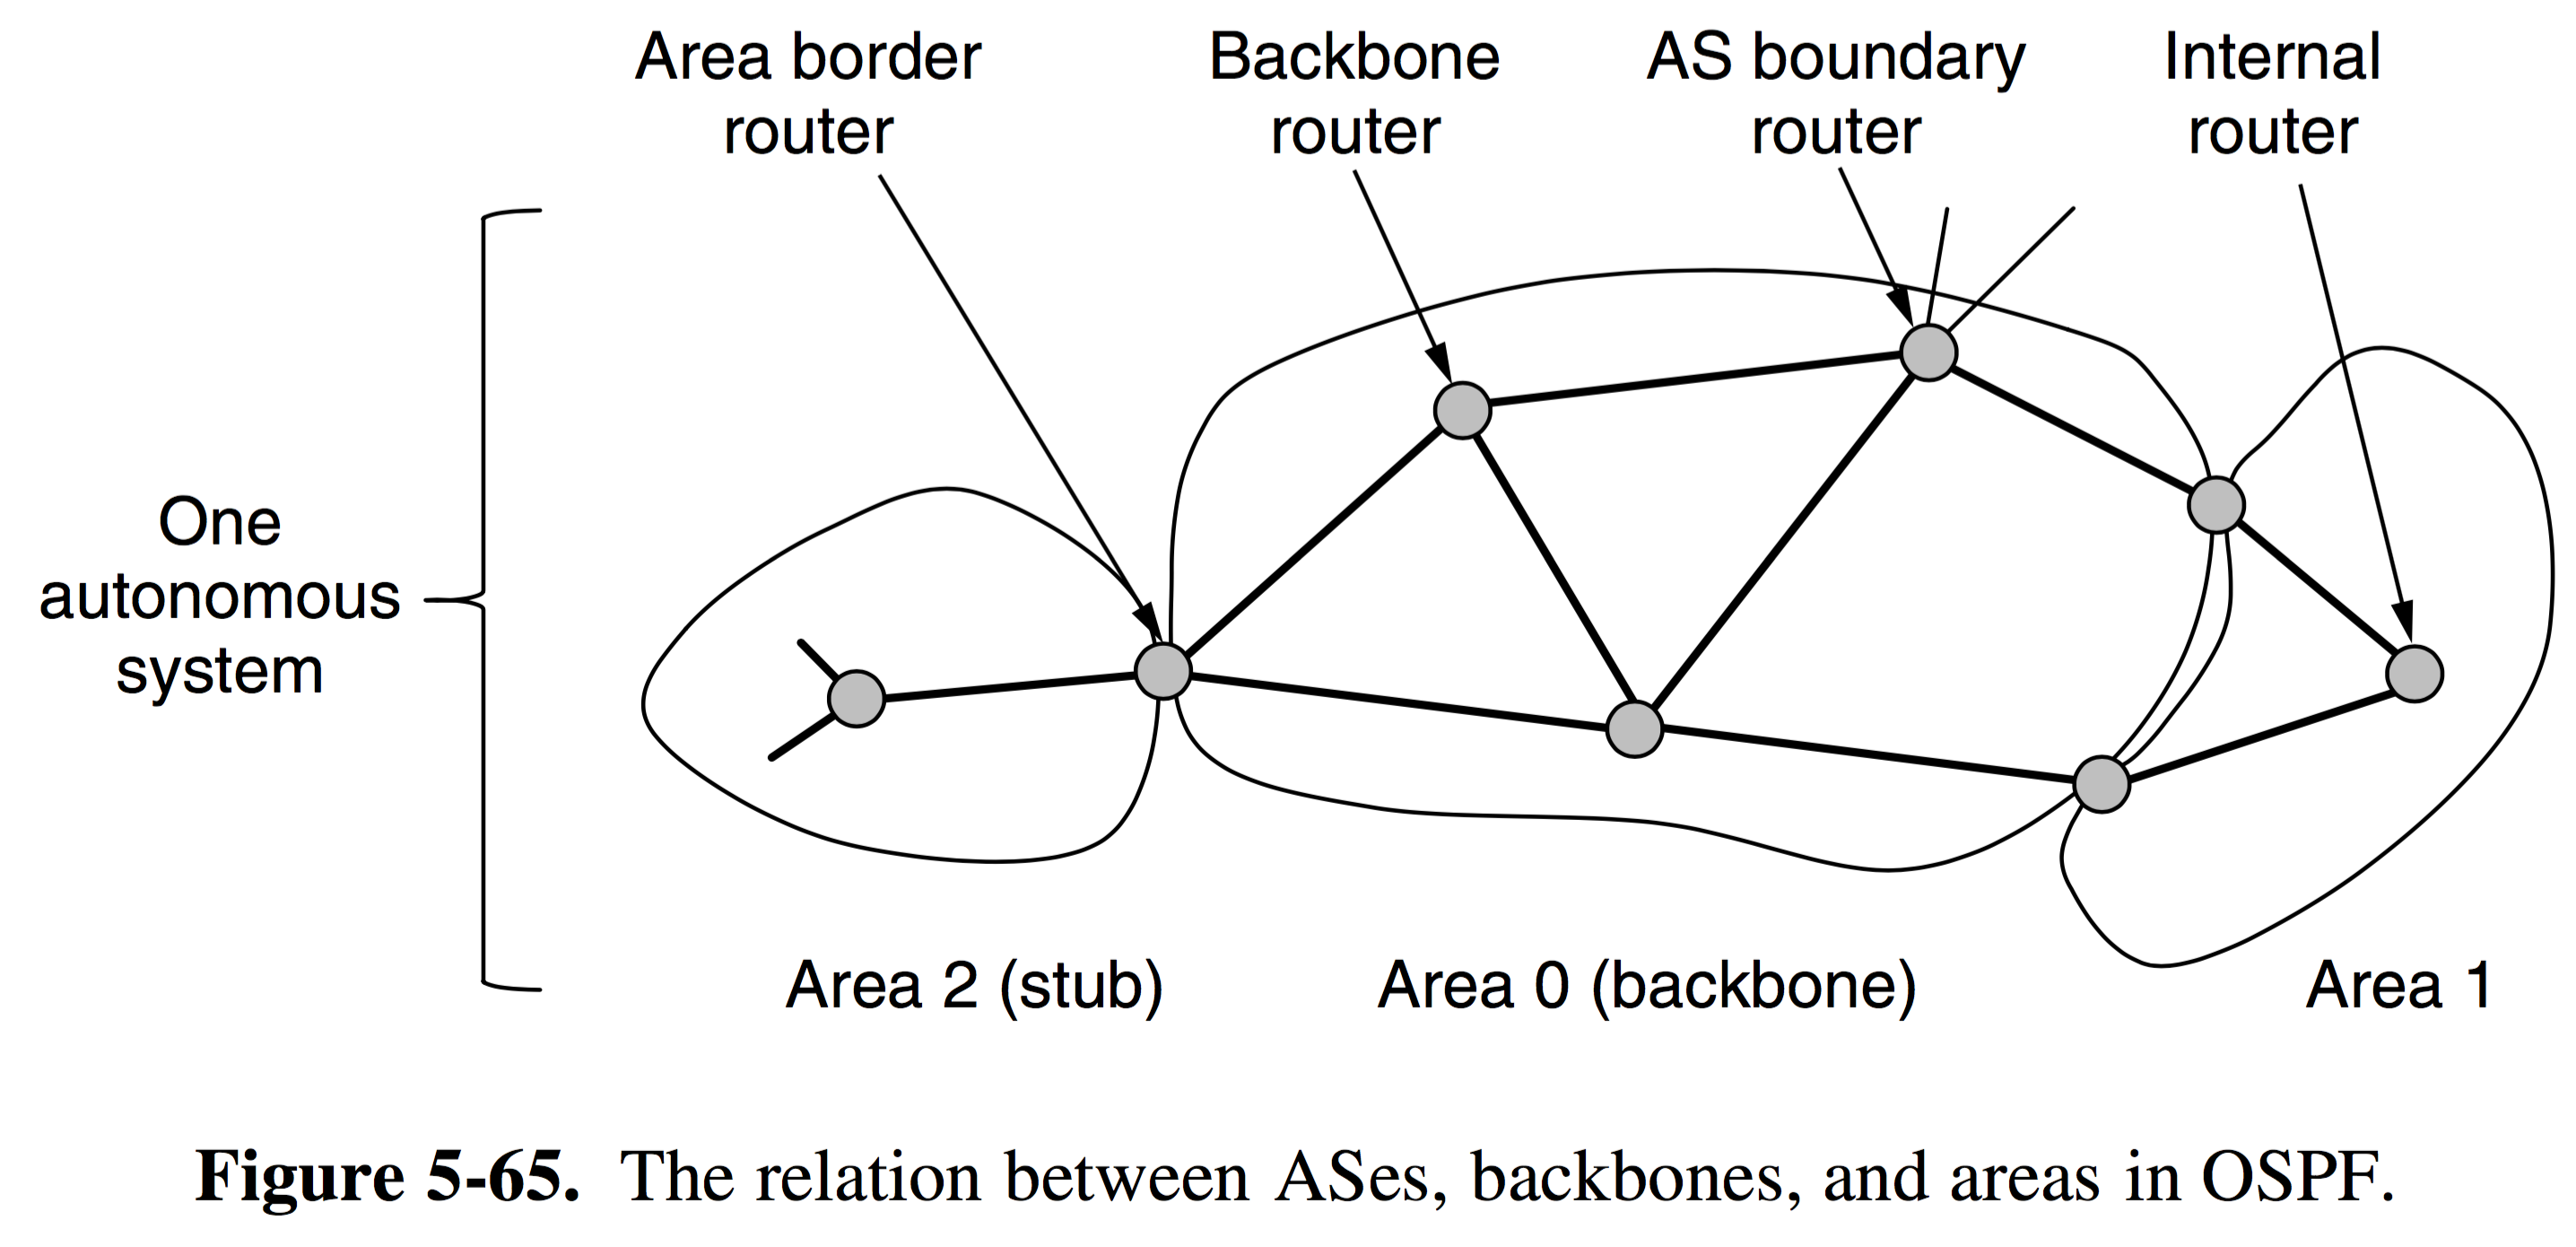
\includegraphics[width=9cm, height=5cm]{./imagenes/ospf2.png} 
		\end{center}
		
	\par Los EBA resumen información de enrutamiento que han aprendido de un área y la hacen disponible en sus avisos de estado de enlace que envían a las otras áreas. Un EBA recibe mensajes de estado de enlace de todos los enrutadores de una de sus áreas A y entonces determina el costo de alcanzar cada red de A. Cuando un EBA envía avisos de estado de enlace a la red dorsal, avisa de los costos de alcanzar las redes del área A, como si estas redes estuvieran directamente conectadas al EBA, esto permite que todos los enrutadores del área dorsal aprendan el costo de alcanzar todas las redes del área A. Cuando un EBA envía avisos de estado de enlace a su red no dorsal, avisa de los costos a alcanzar todas las redes de las otras áreas (no dorsal). Luego todos los enrutadores aprenden a alcanzar todas las redes en el dominio.
	
	\par Cuando se ejecuta OSPF los enrutadores dentro de un área ejecutan el protocolo de estado de enlace, hay paquetes \textbf{Hello}. Los enrutadores dentro de un área intercambian mensajes de estado de enlace periódicamente usando inundación. Estos enrutadores también envían estos mensajes cuando una línea se cae, regresa o su costo cambia. Los mensajes de estado de enlace de enrutadores que no son EBA no dejan el área en el que se originan. Los enrutadores internos a un área no van a conocer detalles acerca de la topología de otras áreas.

	\par Dentro de un área cada enrutador tiene la misma \textbf{base de datos de estado de enlace} (\textit{BDEE}) y ejecuta el mismo algoritmo de la ruta más corta. Su trabajo principal es calcular el camino más corto desde sí mismo a cualquier otro enrutador de su área y red en el AS entero. Un EBA necesita las bases de datos de estado de enlace para todas las áreas a las cuales está conectado y debe correr el algoritmo de Dijkstra para cada área separadamente.


\subsection{BGP: el protocolo de enrutamiento de Puerta de Enlace Exterior}
	
	\par Dentro de un solo sistema autónomo, OSPF e IS-IS son los protocolos de uso común. Entre los sistemas autónomos se utiliza un protocolo diferente, conocido como BGP (\textit{Border Gateway Protocol}). Los protocolos de enrutamiento interdominio tienen que preocuparse en gran manera por la política. Las políticas en cada enrutador de BGP (EBSA) se configuran manualmente. No son parte del protocolo.
	
	\par Los protocolos de puerta de enlace exterior (y BGP en particular) se han diseñado para permitir que se implementen muchos tipos de políticas de enrutamiento en el tráfico entre sistemas autónomos. Las políticas típicas implican consideraciones políticas, de seguridad, o económicas. Algunos ejemplos de posibles restricciones de enrutamiento son:
		\begin{enumerate}
			\item  No transportar tráfico comercial en la red educativa.
			\item Nunca enviar tráfico del Pentágono por una ruta a través de Irak.
			\item Usar TeliaSonera en vez de Verizon porque es más económico.
			\item No usar AT\&T en Australia porque el desempeño es pobre.
			\item El tráfico que empieza o termina en Apple no debe transitar por Google.
		\end{enumerate}
	
	\par Desde el punto de vista de un enrutador de BGP el mundo consiste de sistemas autónomos y las líneas que los conectan. Dos sistemas autónomos se consideran conectados si cada uno contiene un enrutador fronterizo con una línea hacia afuera del sistema autónomo. Una política de enrutamiento es implementada decidiendo qué tráfico puede fluir sobre cuáles enlaces entre SAs.

	\par Un enrutador de frontera de SA (EBSA) tiene la tarea de enviar paquetes entre SAs. BGP corre arriba de TCP. Los pares de enrutadores BGP se comunican entre sí estableciendo conexiones TCP. Proporcionan comunicación confiable y ocultan todo detalle de red que pase a través de ellos.

	\par BGP avisa de caminos completos como una lista enumerada de SA para alcanzar una red particular. Estos avisos hacen falta para detectar ciclos en el enrutamiento y para permitir las decisiones políticas. A los SA se les puede dar números como nombre.
Si un enrutador BGP (EBSA) tiene una elección de varias rutas a un destino, va a elegir la mejor de acuerdo con sus propias políticas locales y esta va a ser la ruta que avisa. Un enrutador BGP no tiene obligación de avisar una ruta a un destino, incluso si tiene una.
Así un SA puede implementar una política de no proveer tránsito, refutando el anuncio de rutas a prefijos que no están contenidos dentro del SA.

	\par Comprender cómo sucede la adaptación a cambios en la topología y en las políticas. Como los enlaces fallan y las políticas cambian, los enrutadores BGP necesitan poder cancelar caminos previamente avisados. Sino los enrutadores BGP van a tener y trabajar con información que ya no sirve o van a violar políticas. Esto se logra con un aviso conocido como \textbf{ruta removida}.

	\par Para enrutamiento inter SA encontrar un camino óptimo es prácticamente 	imposible. Cada SA corre su propio protocolo interno y usa cualquier esquema para 	asignar métricas a los caminos. Es imposible calcular costos de caminos significativos para caminos que cruzan varios SA. El enrutamiento inter SA solo avisa alcanzabilidad, por lo tanto, a lo sumo se pueden tener caminos de SA para ir de un origen a un destino.
	
	\par Para el enrutamiento es necesario encontrar algún camino de SA para el destino  deseado que es libre de ciclos. Además los caminos deben respetar las políticas de los SA a lo largo del camino. Donde una política significa reglas que se refieren a preferencias de enrutamiento y a limitaciones de enrutamiento.
   
	\par Los PPEE suelen implementarse sobre enrutadores de borde de sistema 
   autónomos (EBSA), los cuales tienen que hacer una elección de varias rutas a un 
   destino; va a elegir la mejor de acuerdo con sus propias políticas locales y esta va a 
   ser la ruta que avisa. Además le dice a sus vecinos para cada destino, el camino 
   exacto que está usando.
   	
	\par BGP en cada enrutador para cada destino guarda el registro de la ruta utilizada. El camino consiste del siguiente enrutador de salto (que puede estar en el otro lado del PSI, no adyacente) y la secuencia de SAs que la ruta ha seguido (dada en orden reverso). Cada enrutador de BGP les dice a sus vecinos para cada destino el camino exacto que está usando. Un enrutador que quiere un camino para el destino D, recibe de sus vecinos rutas a D y entre ellas elige la mejor. La regla es que cada enrutador que envía una ruta afuera del SA coloca su propio número de SA en la ruta. Esto explica el porqué la lista está en orden reverso. Llevar el camino completo con la ruta hace fácil para el enrutador receptor detectar y romper ciclos. Cuando un enrutador recibe una ruta la chequea para ver si su propio número de SA ya está en el camino de SAs. Si es así, se ha detectado un ciclo y la publicidad se descarta. Dar una lista de SA es una manera muy gruesa de especificar un camino.

	\par En la siguiente figura hay una red corriendo BGP. Asumimos que los proveedores son redes de tránsito y los clientes son bastones. Un enrutador BGP de SA proveedor A (SA 2) va a poder avisar información de alcanzabilidad para cada uno de los números de red asignados a clientes P y Q.  Así va a decir: “las redes 128.96, 192.4.153, 192.4.32, y 192.4.3 pueden ser alcanzadas dierctamente de SA 2”. La red dorsal, al recibir estos avisos puede avisar: “las redes 128.96, 192.4.153, 192.4.32 y 192.4.3 pueden ser alcanzadas a lo largo del camino (SA 1, SA 3)”

	\begin{center}
		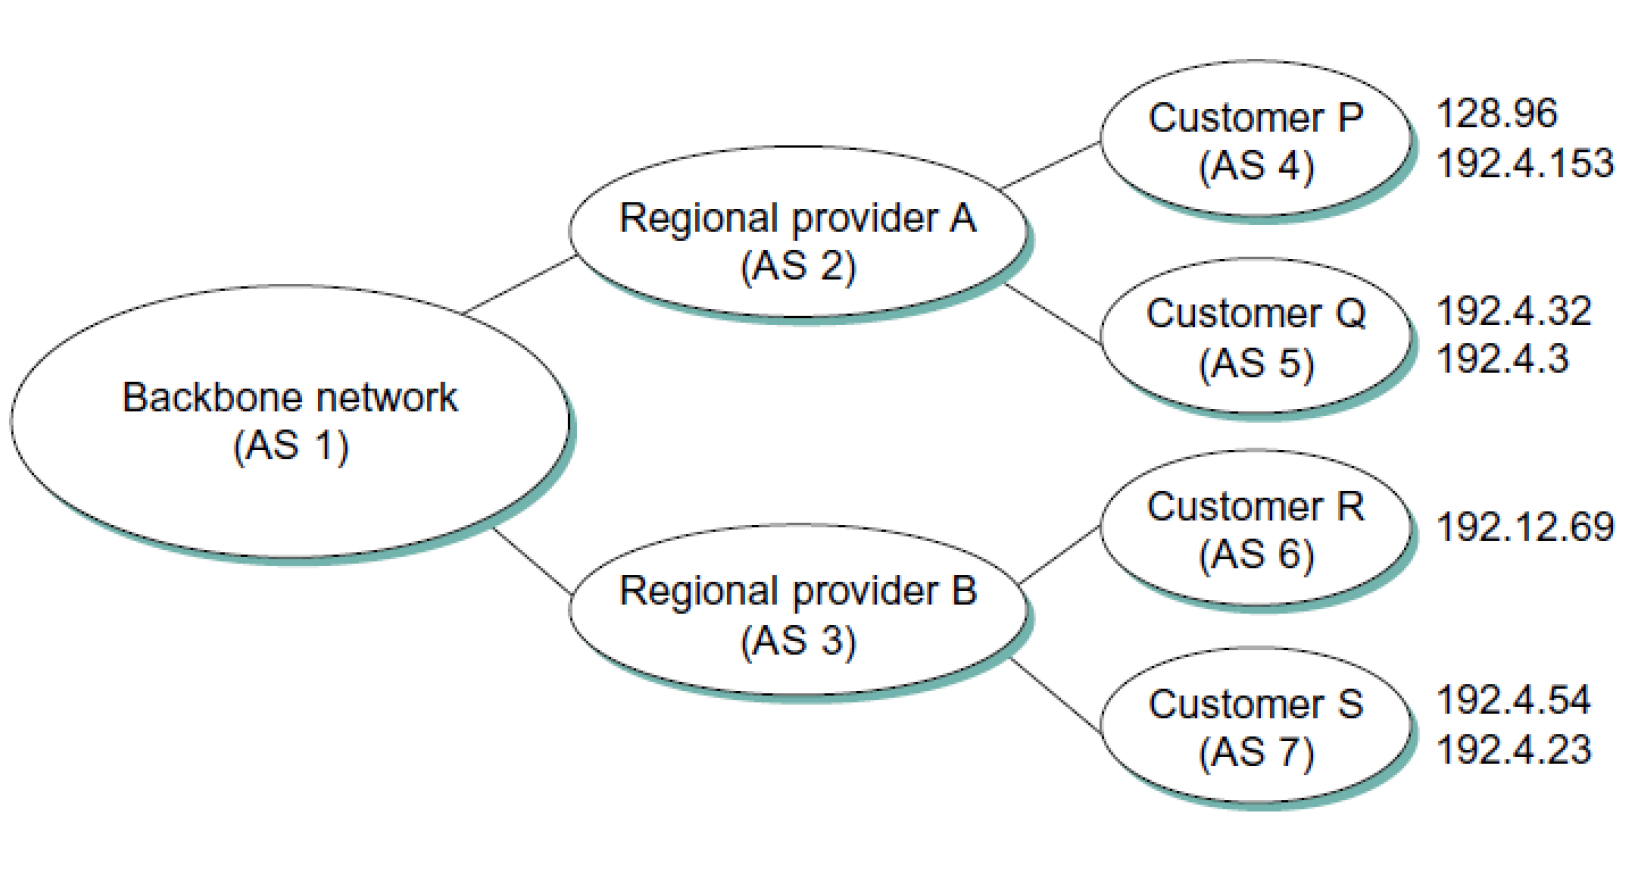
\includegraphics[width=7cm, height=5cm]{./imagenes/fig1.png}
	\end{center}
	
	\par La red de la siguiente figura difiere de la anterior solo en el enlace extra entre SA 2 y SA 3, pero el efecto ahora es que el grafo del SA tiene un ciclo en él. Supongamos que SA 1 aprende que puede alcanzar red 128.96 a través de SA 2, así que avisa este hecho a SA 3, que lo avisa a SA 2. El aviso para el camino a 128.96 recibido por SA 2 de SA 3 va a contener un camino (SA 3, SA 1, SA 2, SA 4), SA 2 se ve a sí mismo en el camino y concluye que este no es un camino útil para usar.

	\begin{center}
		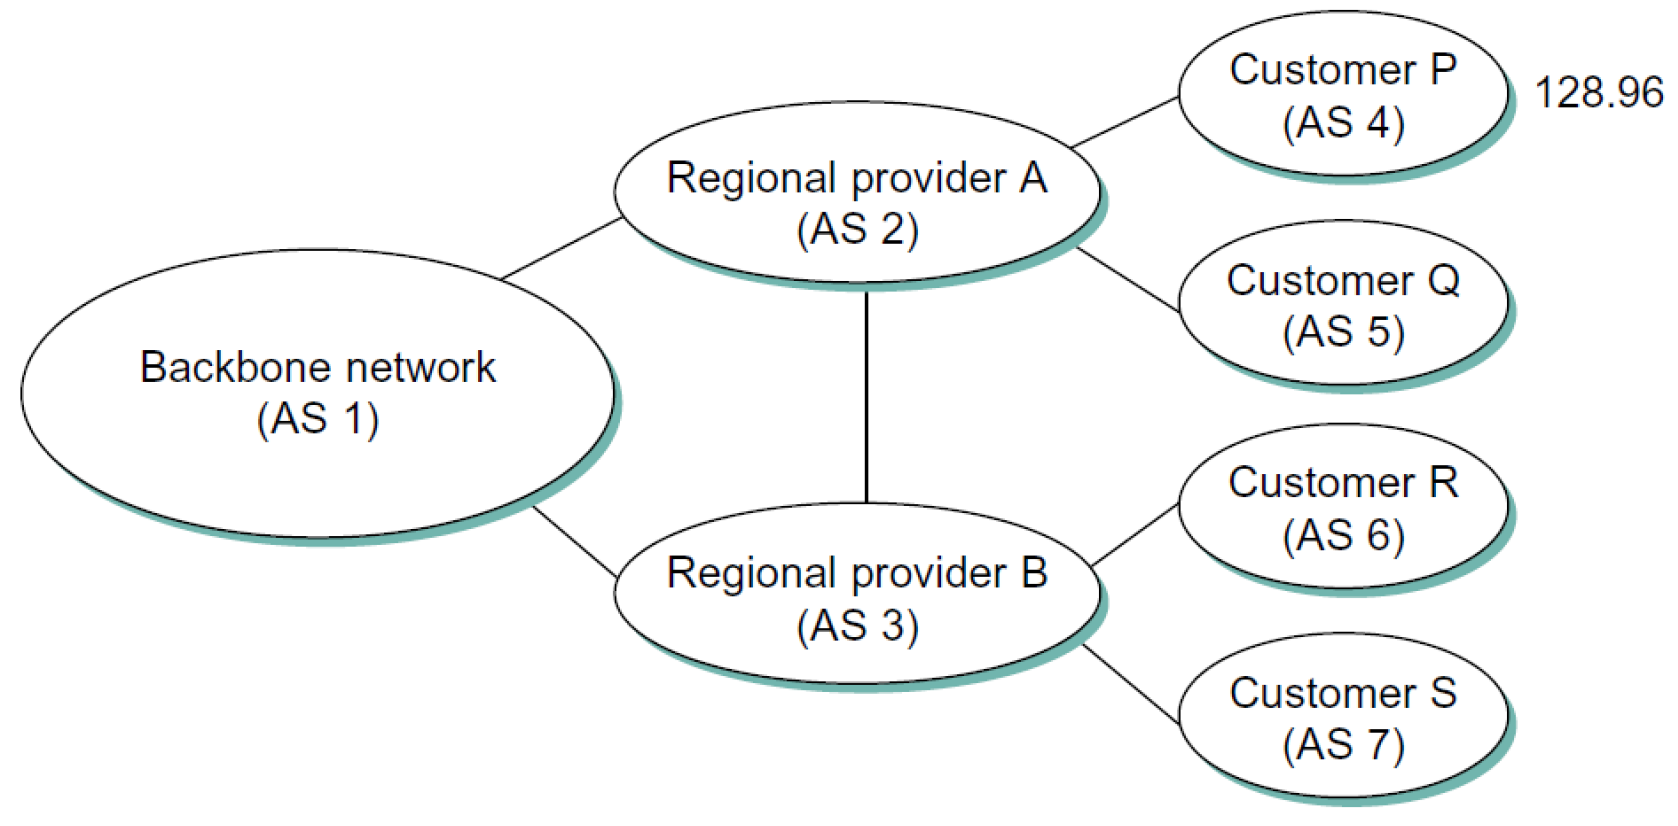
\includegraphics[width=7cm, height=5cm]{./imagenes/fig2.png}
	\end{center}

	\par Los enrutadores no EBSA aprenden información de enrutamiento inter SA porque esa es la función de los enrutadores, enrutar hacia destinos en su SA y hacia los destinos permitidos (respetando políticas) que están en otros SA.

	\par Estrategia: Para resolver el problema haremos un análisis por casos.

	\begin{itemize}
		\item Caso 1: En el caso de un SA bastón que solo conecta a otros SA en un punto simple, el EBSA es la única elección para todas las rutas que están afuera del SA. Tal enrutador puede inyectar una ruta \textit{default} en el protocolo de enrutamiento intra SA.
		\item Caso 2: El siguiente paso en complejidad es tener EBSA que inyecten rutas específicas que ha aprendido de afuera del SA. Ejemplo: Supongamos que un EBSA de un SA proveedor se conecta con un SA cliente. Ese EBSA podría aprender que el prefijo P de red es localizado dentro del SA cliente. Ese EBSA podría inyectar una ruta a P en el protocolo de enrutamiento del SA proveedor. Podría ser un aviso del tipo “tengo un link a p de costo X”. Esto causaría que otros enrutadores en el SA proveedor puedan aprender que este EBSA es el lugar para enviar paquetes a P.
	\end{itemize}

		\par Los SAs dorsales aprenden tanta información de enrutamiento de un enrutador BGP que se convierte en demasiado caro inyectarla en el protocolo intra SA. Ejemplo: si el EBSA quiere inyectar 10.000 prefijos que ha aprendido de otro SA, va a tener que enviar paquetes de estado de enlace muy grandes a los otros enrutadores en ese SA y los cálculos de caminos más cortos van a ser muy costosos.

	\par Los enrutadores en una SA dorsal usan una variante de BGP llamada interior BGP (iBGP) para redistribuir efectivamente la información que ha aprendido por los enrutadores BGP en los arcos de los SA a todos los demás enrutadores del SA. iBGP permite a cada enrutador en el SA aprender el mejor EBSA para usar cuando envía un paquete a cualquier dirección. Al mismo tiempo, cada enrutador en el SA mantiene la pista de cómo ir a cada EBSA usando un protocolo convencional intra SA sin información inyectada. Combinando estos dos conjuntos de información cada enrutador en el SA puede determinar el salto próximo apropiado para todos los prefijos.

	\par La tabla arriba a la izquierda de la siguiente figura muestra la información que el enrutador B aprende de sus sesiones iBGP. Aprende que algunos prefijos son mejor alcanzados por el enrutador A, otros vía D y algunos vía E (ver SA de figura anterior). Al mismo tiempo todos los enrutadores en el SA ejecutan OSPF y del mismo B aprende cómo alcanzar otros nodos dentro del dominio, como se ve en la tabla de arriba a la derecha. Finalmente en la tabla de abajo, B pone el cuadro completo combinando la información acerca de prefijos externos aprendidos de iBGP con la información acerca de rutas internas a los enrutadores de borde aprendida de OSPF.
	
	\begin{center}
		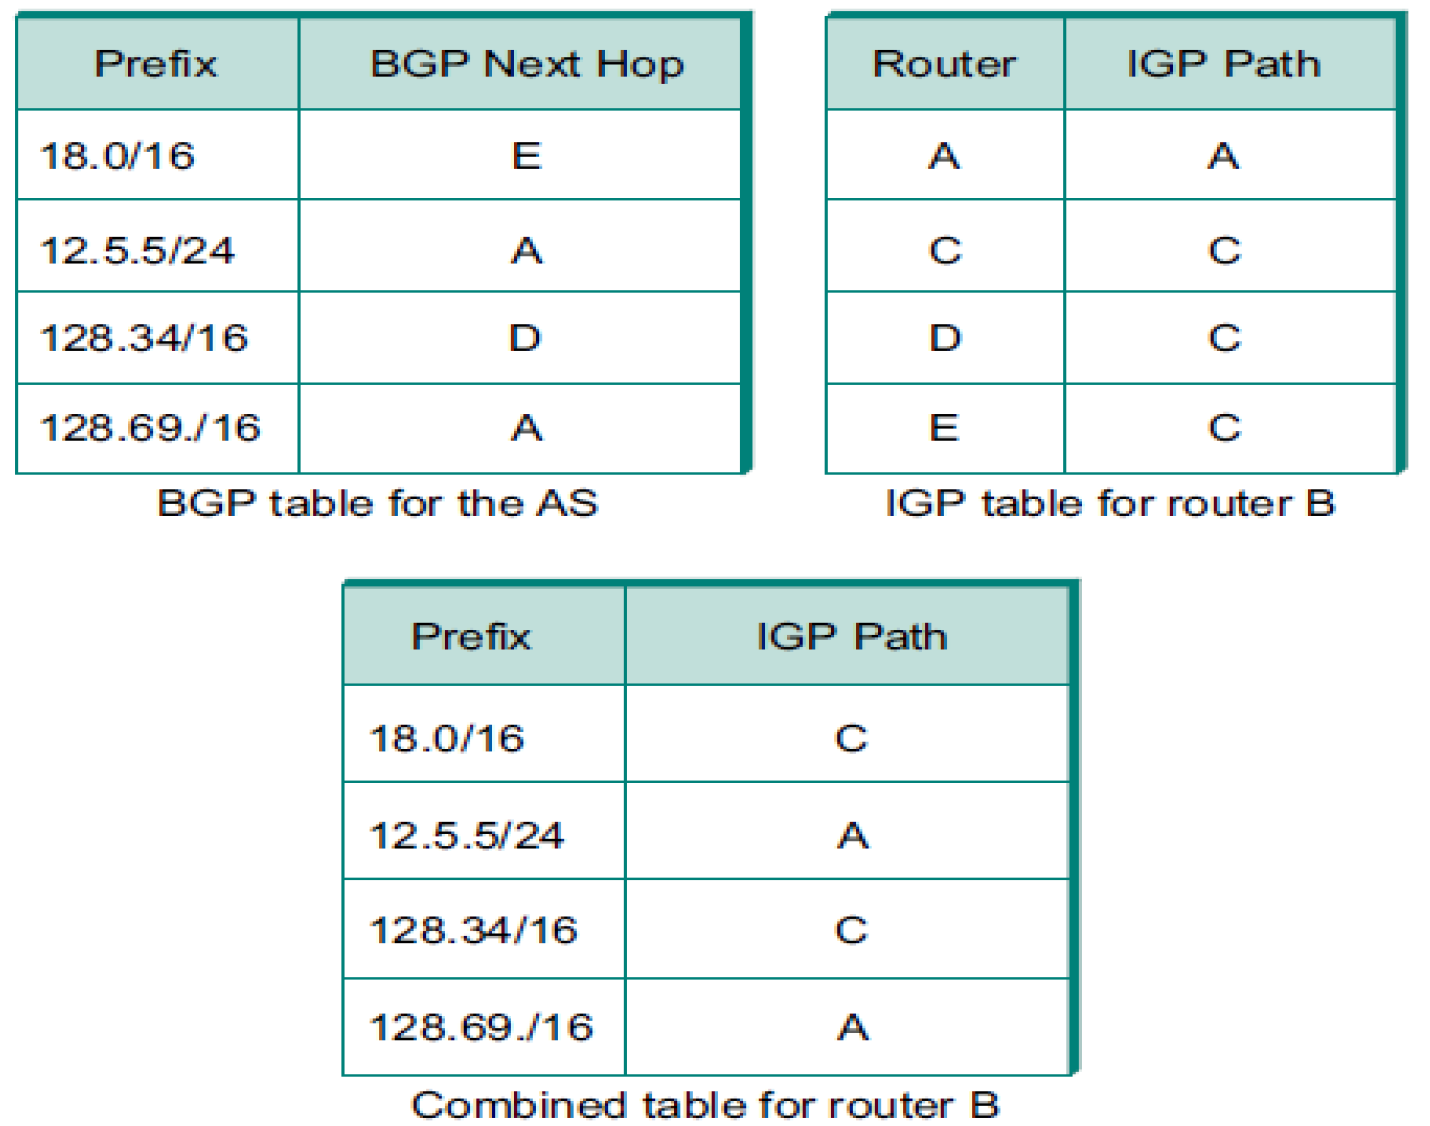
\includegraphics[width=7cm, height=5cm]{./imagenes/fig3.png}
	\end{center}

	\par Cada enrutador BGP puede aprender una ruta para un destino dado del enrutador con el cual está conectado en el próximo PSI y de todos los otros enrutadores frontera (los cuales han escuchado diferentes rutas de los enrutadores con los cuales están conectados en otros PSI). Cada enrutador debe decidir cuál ruta en este conjunto de rutas es la mejor a usar. Está a cargo del PSI escribir alguna política para recolectar la ruta preferida. Vamos a describir algunas estrategias comunes.

	\begin{itemize}
		\item Estrategia 1: Las rutas vía redes compañeras se eligen en preferencia a las rutas vía proveedores de tránsito.
		\item Estrategia 2: A las rutas del cliente se les da la mayor preferencia.
		\item Estrategia 3: (regla por \textit{default}) caminos SA más cortos son mejores.
		\item Estrategia 4: es preferible la ruta que tiene el costo más corto dentro del PSI.
	\end{itemize}

	\par Cada enrutador BGP contiene un módulo que examina las rutas a un destino dado y las califica, devolviendo un número para la “distancia” a ese destino por cada ruta. Cualquier ruta que viole una restricción de la política recibe automáticamente una calificación al infinito. Entonces el enrutador adopta la ruta de la distancia más corta al destino. La función de calificar no es parte del protocolo de BGP y la fija el administrador del sistema. Ahora damos algunos detalles importantes adicionales de la implementación de BGP. Cada enrutador BGP mantiene una base de datos de redes que puede alcanzar y la ruta preferida para alcanzar cada red. Cuando se hace un cambio a esta base de datos, el enrutador BGP construye un mensaje de actualización (\textit{update}) que es difundido a todos los otros enrutadores implementando BGP. De este modo todos los enrutadores BGP pueden construir y mantener su información de enrutamiento.

	\par El mensaje de actualización comunica dos tipos de información:
Información acerca de una ruta simple a través de la internet. La misma está disponible para ser agregada en la base de datos de todo enrutador BGP receptor. Una lista de rutas previamente avisadas por este enrutador que ya no son más válidas. Un mensaje de actualización puede contener ambos o uno de esos tipos de información.

	\par La información acerca de una ruta simple consiste de los siguientes campos:
	\begin{itemize}
		\item Lista de identificadores de las redes que pueden ser alcanzadas por esa ruta. El identificador de una red es su dirección IP, que es una porción de una dirección IP completa.
		\item Los atributos del camino. Lista de SAs que son recorridos por esa ruta, dirección IP del EBSA que se va a usar como próximo salto a los destinos del campo anterior.
	\end{itemize}
	
	\par Para dar la lista de rutas previamente avisadas a cancelar, basta con identificar cada una de esas rutas con la dirección IP de una red de destino.
	
	\par Muchos PSI existen solo para proveer servicios a consumidores (Ej: redes 
	hogareñas). Otros PSI ofrecen algo parecido a un servicio dorsal interconectando 
	otros PSI y a veces grandes corporaciones. La política en la cual dos SA mandan tráfico directamente entre sí en forma gratuita, se conoce como \textbf{compañerismo}. A menudo varios proveedores se conectan entre sí como un punto único de compañerismo.
	
	\par \textbf{Relación de compañerismo:} Para lograr esto los dos SA mandan publicidad de enrutamiento de uno al otro para las direcciones que residen en sus redes. El compañerismo no es transitivo.
	
	\par \textbf{Relación proveedor-consumidor:} Una política común es que un PSI paga a otro PSI para entregar paquetes a otros destinos en la internet y recibir paquetes enviados de otros destinos. El PSI cliente se dice que compra servicio de tránsito del PSI proveedor y debe dar publicidad de rutas (a todos los destinos en internet) al cliente sobre el enlace que lo conecta. De este modo, el cliente va a tener una ruta para usar para enviar paquetes para todos lados. El PSI cliente debe publicar rutas (a los destinos en su red) al PSI proveedor. Esto va a permitir al proveedor enviar tráfico al cliente solo para esas direcciones.

	\par Algunos PSI están conectados a varios PSI, esta técnica (llamada \textit{multihoming}) es usada para mejorar la confiabilidad, por si el camino por uno de los PSI falla.

	\par \textbf{Definiciones:}
	\begin{itemize}
		\item \underline{Tráfico local:} tráfico que se origina y termina en nodos dentro de un SA. 		
		\item \underline{Tráfico de tránsito:} tráfico que pasa a través de un SA.
	\end{itemize}

	\par Los SA se agrupan en categorías:
	\begin{itemize}
		\item \textbf{SA bastón (stub):} tienen solo una conexión con el grafo de BGP. No se pueden usar para transportar tráfico porque no hay nadie en el otro lado.
		\item \textbf{SA multi-homed:} un SA que tiene una conexión a más de un SA pero que rechaza llevar tráfico de tránsito.
		\item \textbf{SA multi-conectadas:} se pueden usar para el transporte de tráfico excepto que lo rechacen.
		\item \textbf{SA de tránsito:} (como redes dorsales) están dispuesta a ocuparse de paquetes de terceros, posiblemente con algunas restricciones, y normalmente por pago.
	\end{itemize}
